%% Template.tex; Solar Physics
%% 
\documentclass[namedreferences]{solarphysics}
%
% spr-sola-addons available options:
%  hyperref      -- loads hyperref.sty with options (pdfborder={0 0 0 },urlcolor=blue,breaklinks)
%  nonatbib      -- do not load natbib.sty (style loads it by default)
%  solaromanenum -- makes enumerated list with roman numerals and a single right-bracket
%  linksfromyear -- puts a link on a year citation (hyperref must be loaded). Loaded by default
%  nolinksfromyear -- suppress  linksfromyear
%  optionalrh    -- for optional running title/author
%  showbiblabels -- to show bibitem label at end of bibitem (via \endbibitem command)
%
\usepackage[hyperref,optionalrh,solaromanenum]{spr-sola-addons} % For Solar Physics 
%\usepackage{epsfig}                     % For eps figures, old commands
\usepackage{graphicx}                    % For eps figures, newer & more powerfull
%\usepackage{courier}                    % Change the \texttt command to courier style
\usepackage{amssymb}                    % useful mathematical symbols
\usepackage{color}                       % For color text: \color command
\usepackage{breakurl}                         % For breaking URLs easily trough lines
\def\UrlFont{\sf}                        % define the fonts for the URLs
\usepackage{comment}
\usepackage{setspace}

%% Local definitions
%% please place your own definitions here and don't use \def but
%% \newcommand{}{} or 
%% \renewcommand{}{} if it is already defined in LaTeX
\renewcommand{\deg}{$^\circ$}
\newcommand{\mdeg}{^\circ}
\newcommand{\rsun}{R{$_\odot$}}
\renewcommand{\l}{\lambda_{\rm N}}%\lambda_
\newcommand{\mrsun}{{\rm R_\odot}}
\newcommand{\med}{{\rm Md}}
\newcommand{\avgTe}{\left<T_\textrm{m}\right>}
\newcommand{\MK}{{\rm MK}}
\newcommand{\cm}{{\rm cm}}
\newcommand{\sdev}{{\rm SD}}
\newcommand{\mean}{{\rm Mn}}
\newcommand{\deltat}{$\delta$}
\newcommand{\LDEM}{{\rm LDEM}}
\newcommand{\FBE}{{\rm FBE}}
\newcommand{\TRF}{{\rm TRF}}
\newcommand{\lN}{\lambda_N}
\newcommand{\NCB}{N_{\rm CB}}
\newcommand{\aTm}{\left< T_\textrm{m}\right>}
\newcommand{\Nqi}{N_{\rm QI}}

\newcommand{\Tefit}{T_{e,{\rm fit}}}

\newcommand{\BibTeX}{\textsc{Bib}\TeX}
\newcommand{\etal}{{\it et al.}}


%%%%%%%%%%%%%%%%%%%%%%%%%%%%%%%%%%%%%%%%%%%%%%%%%%%%%%%%%%%%%%%%%%
\begin{document}

\begin{article}

\begin{opening}

\title{Thermodynamic Structure of the Solar Corona: Tomographic Reconstructions and MHD Modeling}

%%%%%%%%%%%%%%%%%%%%%%%%%%%%%%%%%%%%%%%%%%%%%%%%%%%
%% Authors Names
%
% \author[addressref={},corref,email={}]{\inits{}\fnm{}\lnm{}\orcid{}}
\author[addressref={aff1,aff2},corref,email={dlloveras@iafe.uba.ar}]{\inits{D.G.}\fnm{Diego G.}~\lnm{Lloveras}\orcid{0000-0003-1402-0398}}

\author[addressref={aff1,aff3,aff2},corref,email={albert@iafe.uba.ar}]{\inits{A.M.}\fnm{Alberto M.}~\lnm{V\'asquez}\orcid{0000-0003-3401-6409}} 

\author[addressref={aff1,aff2},corref,email={federico@iafe.uba.ar}]{\inits{F.A.}\fnm{Federico A.}~\lnm{Nuevo}\orcid{0000-0003-2355-5853}} 

\author[addressref={aff1,aff3,aff2},corref,email={cmaccormack@iafe.uba.ar}]{\inits{C.}\fnm{Cecilia}~\lnm{Mac Cormack}}

\author[addressref={aff4},corref,email={nishthas@umich.edu}]{\inits{N.}\fnm{Nishtha}~\lnm{Sachdeva}\orcid{1}}

\author[addressref={aff4},corref,email={chipm@umich.edu}]{\inits{W.}\fnm{Ward}~\lnm{Manchester IV}\orcid{2}}

\author[addressref={aff4},corref,email={bartvand@umich.edu}]{\inits{B.}\fnm{Bartholomeus}~\lnm{Van der Holst}\orcid{3}}

\author[addressref={aff4},corref,email={rfrazin@umich.edu}]{\inits{R.A.}\fnm{Richard A.}~\lnm{Frazin}\orcid{0000-0002-0281-7677}}

%%%%%%%%%%%%%%%%%%%%%%%%%%%%%%%%%%%%%%%%%%%%%%%%%%%
%% Runningheads
%
\runningauthor{D.G.~Lloveras~\etal}
%\runningtitle{}


%%%%%%%%%%%%%%%%%%%%%%%%%%%%%%%%%%%%%%%%%%%%%%%%%%%
%% Affilations 
%% id shold be the same with \author addressref value.
%\address[id={}]{}
\address[id=aff1]{Instituto de Astronom\'{\i}a y F\'{\i}sica del Espacio (IAFE), CONICET-UBA, CC 67 - Suc 28,  (C1428ZAA) Ciudad Aut\'onoma de Buenos Aires, Argentina}

\address[id=aff2]{Departamento de F\'{\i}sica, Facultad de Ciencias Exactas y Naturales (FCEN), Universidad de Buenos Aires (UBA), Pabell\'on I, Ciudad Universitaria, (C1428ZAA) Ciudad Aut\'onoma de Buenos Aires, Argentina}

\address[id=aff3]{Departamento de Ciencia y Tecnolog\'{\i}a, Universidad Nacional de Tres de Febrero (UNTREF), Valent\'{\i}n G\'omez 4752, (B1678ABH) Caseros, Provincia de Buenos Aires, Argentina}

\address[id=aff4]{Department of Climate and Space Sciences and Engineering (CLaSP), University of Michigan, 2455 Hayward Street, Ann Arbor, MI 48109-2143, USA}
%%%%%%%%%%%%%%%%%%%%%%%%%%%%%%%%%%%%%%%%%%%%%%%%%%%
%%% Abstract 
\begin{abstract}
Observational tools play an essential role in advancing our understanding of the physics of the solar corona. They provide validation data to improve three-dimensional (3D) magnetohydrodynamic (MHD) models of the solar atmosphere, key to enhance their space weather forecasting capabilities. Solar rotational tomography (SRT) is currently the sole observational technique that provides an empirical 3D description of fundamental plasma parameters of the solar corona at a global scale. Based on EUV data of space borne instruments, SRT allows constructing 3D maps of the coronal electron density and temperature at heliocentric heights below 1.25 Rsun. We carry out a study of the corona combining tomographic reconstructions with MHD simulations of the latest version of the Alfv\'en Wave Solar Model (AWSoM) of the Space Weather Modeling Framework (SWMF). Target rotations were selected from the solar minimum between solar cycles (SC) 23 and 24 and the current declining phase of solar cycle 24. Tomographic reconstructions and results of the model are analyzed in distinct coronal magnetic structures. We study magnetically closed structures associated with the equatorial streamer belt, as well as magnetically open regions enclosing it. We report on the tomographic results in the different structures, their implications for the physics of the solar corona, and the capability of the AWSoM model to reproduce the tomographic reconstructions in different regions.

\end{abstract}



%%%%%%%%%%%%%%%%%%%%%%%%%%%%%%%%%%%%%%%%%%%%%%%%%%%
%% Keywords
%
\keywords{Solar Cycle, Observations; Corona,E; Corona, Structures}


\end{opening}
%-------------------------------------------------

%%%%%%%%%%%%%%%%%%%%%%%%%%%%%%%%%%%%%%%%%%%%%%%%%%%
%% Sections
\section{Introduction}\label{intro} 

Being the place where the solar atmosphere is heated and the solar wind accelerated, and where impulsive events such as solar flares and coronal mass ejections are energized, observation and modeling of the solar corona are tasks of great relevance to improve our understanding of the Sun-Earth environment. To advance our knowledge of the physics of the solar corona, as well as to improve its three-dimensional (3D) models, information derived from observational data plays a key role. Solar rotational tomography is currently the sole observational technique able to provide a quantitative empirical description of the 3D distribution of some fundamental plasma parameters of the solar corona at a global scale.


\section{Methodology}\label{meto}   

\subsection{DEMT reconstructions}\label{demt} 
\textcolor{red}{*Tratado de imagenes}
\textcolor{red}{*FBE}
\textcolor{red}{*LDEM}


Once the LDEM is determined at each voxel, the average squared electron density $\langle N_e^2 \rangle$ and the electron mean temperature $T_\textrm{m}$ in the voxel can be computed by taking its zeroth and first moments over temperature. More specifically, at the $i$-th voxel,
\begin{eqnarray}\label{momento1}
 \langle N_{e,i}^2 \rangle &=& \int\,\textrm{d}T\,\LDEM_i(T),\label{Ne} \\ 
\label{momento2}
 T_{\textrm{m},i}   &=& \frac{1}{\langle N_{e,i}^2 \rangle}\,\int\,\textrm{d}T\,T\,\LDEM_i(T),\label{Tm} 
\end{eqnarray}


so that the final product of DEMT is in the form of 3D maps of the electron density and mean temperature. These relationships was derived in detail in \citealt{frazin_2009} (see Appendix C). 

\textcolor{red}{*aclarar que consideramos Ne como $\sqrt{<N_e ^2>}$.}

\textcolor{red}{*Mejoras de la tecnica con respecto a trabajos previos}

\subsection{AWSoM simulations}\label{awsom} 
\textcolor{red}{*Que es, que modela, que datos usa, y que se obtiene en general y en particular para este trabajo}


\subsection{Tracing results along fieldlines}\label{trace} 

For both rotations, the DEMT and AWSoM 3D maps of electron density $N_e$, electron mean temperature $T_\textrm{m}$ and electron temperature $T_\textrm{e}$ respectively were traced along the magnetic field lines modeled using AWSoM as described at the end of Section \ref{awsom}. In the case of closed loops, results were separated into their two legs, defined as the two segments that go from the coronal base up to the apex.


\textcolor{red}{Se eligen loops con abs(person temp) mayor a .5 lo cual nos permite descartar loops QI.
OBS: Esto es valido para hasta la fig 7 inclusive.}


For each open field line, and for each leg of the closed ones, an exponential fit was then applied to the $N_e(r)$ data points, and a linear fit applied to the $T_m(r)$ data points, as described by

\begin{eqnarray}\label{Nfit}
N_e &=& N_0\,\exp{\left[\,-\,\left(h/\l\right)\,/\,\left(r/\mrsun\right)\,\right]}\\
\label{Tfit}
T_\textrm{m} &=& a\,r\,+\,b
\end{eqnarray}
 
\noindent
where $h \equiv r - 1\,\mrsun$, and $a$ and $b$ are constants. 

In the case of the electron density, the fitted function corresponds to the isothermal hydrostatic equilibrium solution, allowing for variation of the solar gravitational acceleration with height. After computing the footpoint ($r=1.0\,\mrsun$) electron density $N_{0}\,[\cm^{-3}]$ and scale height $\lN\,[\mrsun]$\textcolor{blue}{, this choice of function provides a straightforward means to directly evaluate how compatible is the observed coronal thermodynamical state with the hydrostatic solution}. The linear fit allows characterization of its variation with height by means of a characteristic temperature gradient $a = \textrm{d}T_m/\textrm{d}r\,[\MK/\mrsun]$ along each leg.



DEMT has been improved since the previously published work. We now perform hollow-tomography with the EUV images, \textcolor{red}{definir hollow-tom} and a 3D regularized of the solution was applyed to obtain smother and more reliable result at the edge of the tomographic grid.

\textcolor{red}{*Nos quedamos con los fiteos que cumplen test de hipotesis chi cuadrado en temp y densidad.
OBS: Esta es la seleccion para las figuras 8 en adelante. Citar numerical recipes seccion 15.2}


For the two targeted rotations, DEMT and AWSoM resuls were traced along the AWSoM field lines, which provides a way to characterize the global thermodynamic state of the inner solar corona and to compare them. To that end three different types of magnetic lines corresponding with three different types of magnetic structures where selected:

  0 - Small-closed field lines footlat $<30$ y gradt neg. where most of the DOWN loops showed up before

  I - Small-closed field lines. Small meaning with apex within the DEMT range of heights. gradt pos
   %This class thoroughly probes the inner core of the Streamer belt, where most of the DOWN loops showed up before, and will show up now.

  II - Large-closed field lines. Large meaning their apex surpasses the DEMT range of heights. This class is mostly populated by very large trans-equatorial field lines forming the "envelope" of the Streamer belt. footlat $>30$ y gradt pos

 III - Open field lines. footlat $>60$ y gradt pos

\textcolor{red}{que quede claro que de ahora en mas solo consideramos ajustes de loops up, es decir pearson temp > 0.5 debido a que awsom solo tiene up.}


\section{Results}\label{resu} 

\subsection{Tomographic Results}\label{demt_res} 

Once the LDEM was determined for each rotation, the electron density $N_e$ and electron mean temperature $T_\textrm{m}$ were computed at each voxel of the tomographic computational grid by means of Equations \ref{momento1} and \ref{momento2}. As an example, Figures \ref{carmaps_demt_2082} and \ref{carmaps_demt_2208} show the results for both rotations at $r=1.025, 1.065$ and $1.105\,\mrsun$. Black voxels correspond to non-reconstructed regions.

\textcolor{red}{
*explicar voxel negros
*Comentarios descriptivos sobre las rotaciones:
-Simetria
-CH
-Matcheo entre open-closed boundaries y las estructuras termodinamicas.
}


\begin{figure}[h!]
\begin{center}
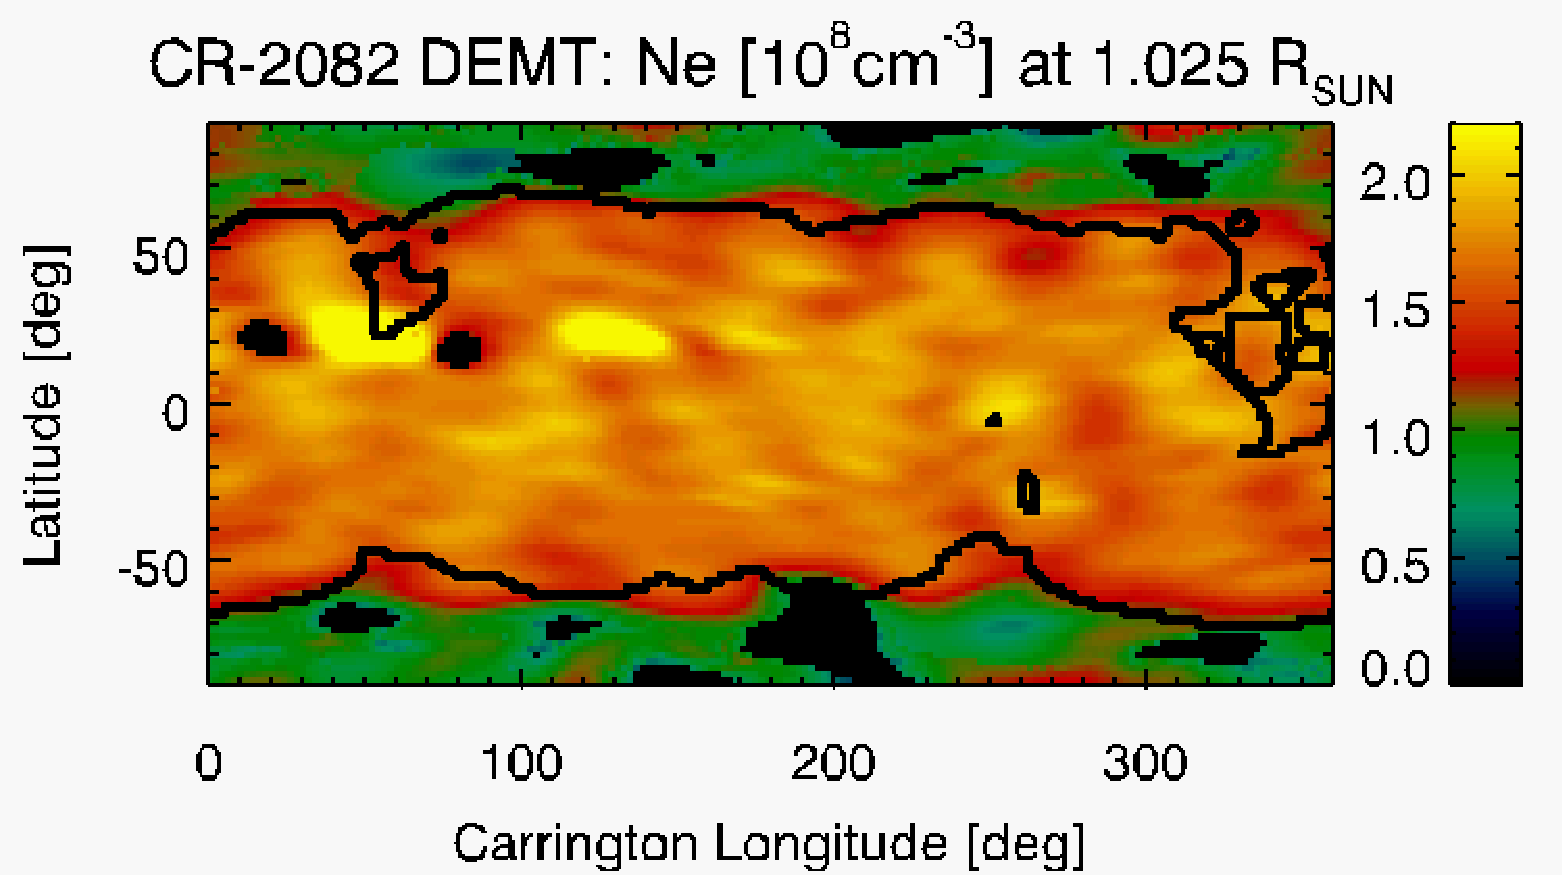
\includegraphics[width=0.495\textwidth]{figs/map_Ne_CR2082_DEMT-EUVI_behind_H1-L3523_r3d_1025_Rsun.pdf}
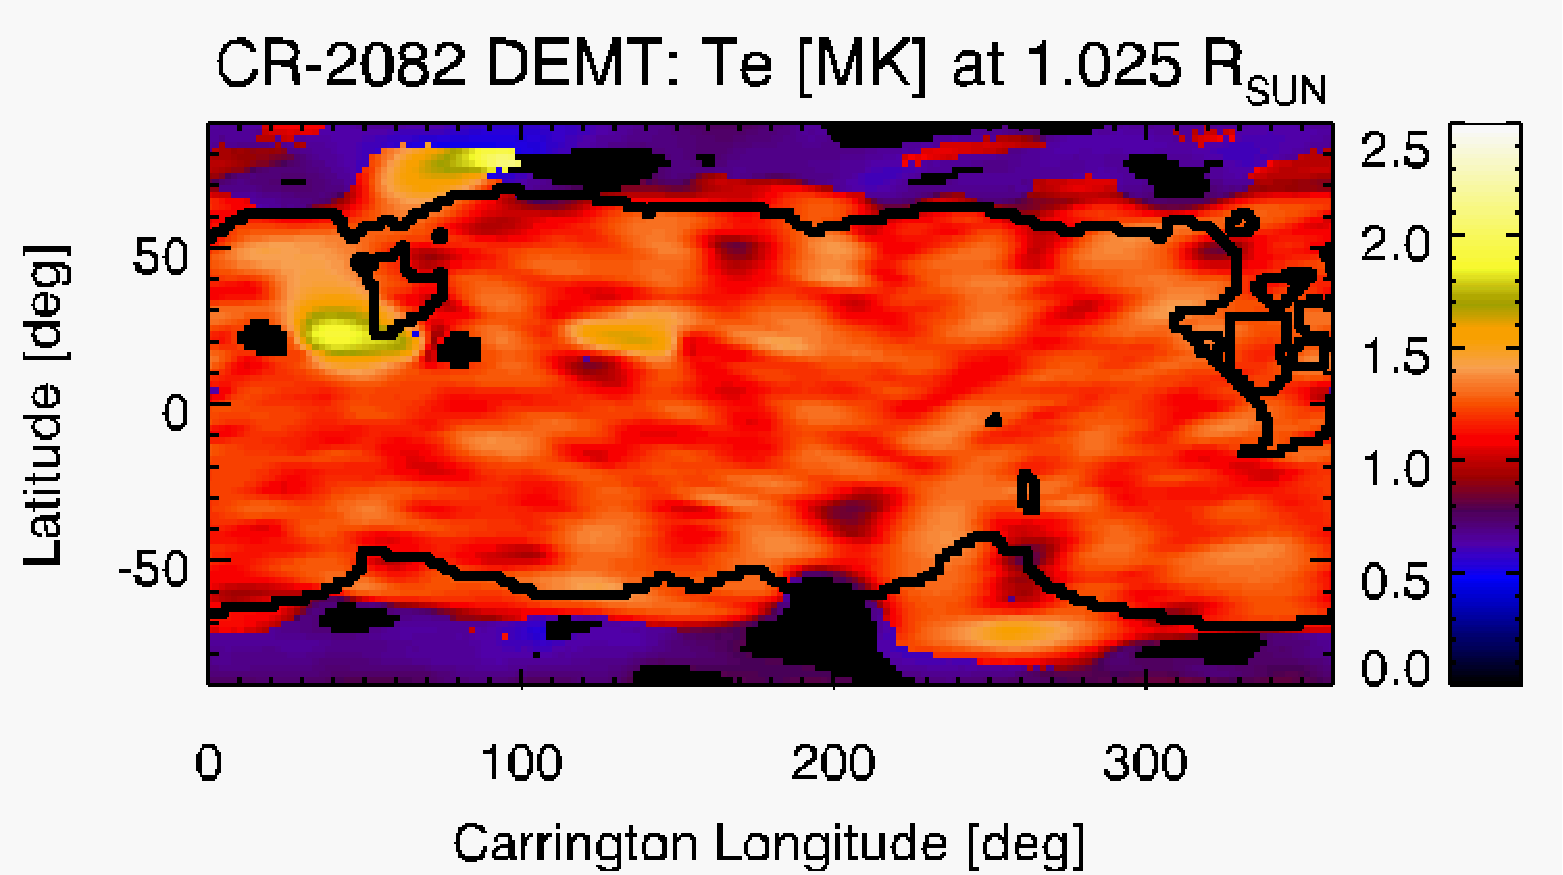
\includegraphics[width=0.495\textwidth]{figs/map_Tm_CR2082_DEMT-EUVI_behind_H1-L3523_r3d_1025_Rsun.pdf}
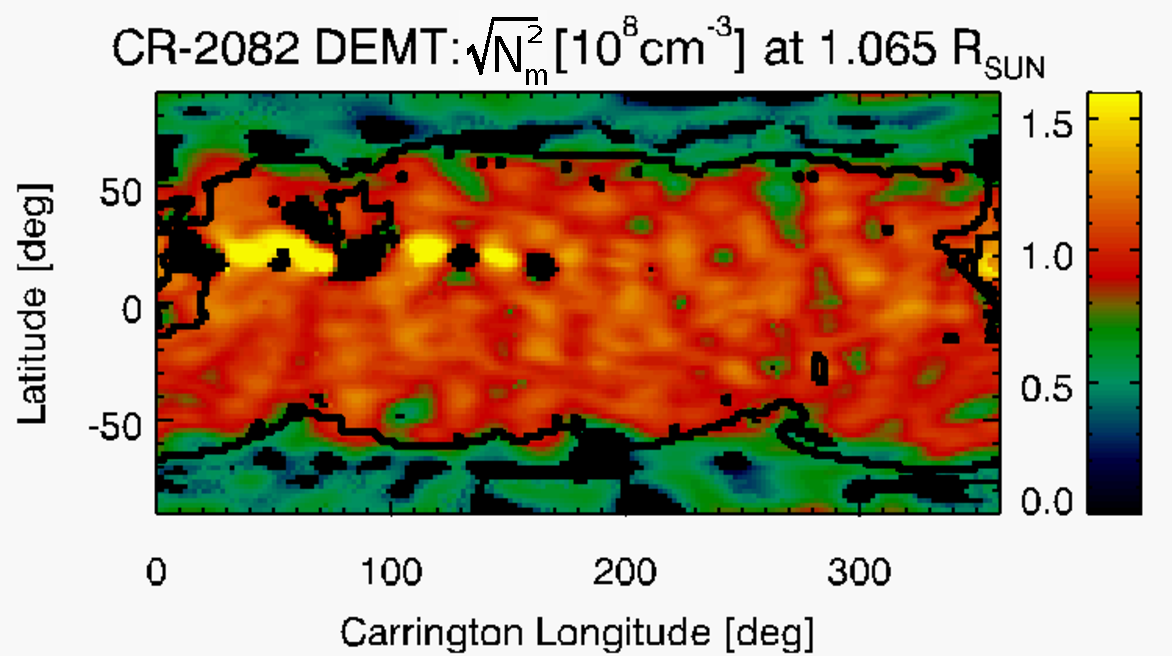
\includegraphics[width=0.495\textwidth]{figs/map_Ne_CR2082_DEMT-EUVI_behind_H1-L3523_r3d_1065_Rsun.pdf}
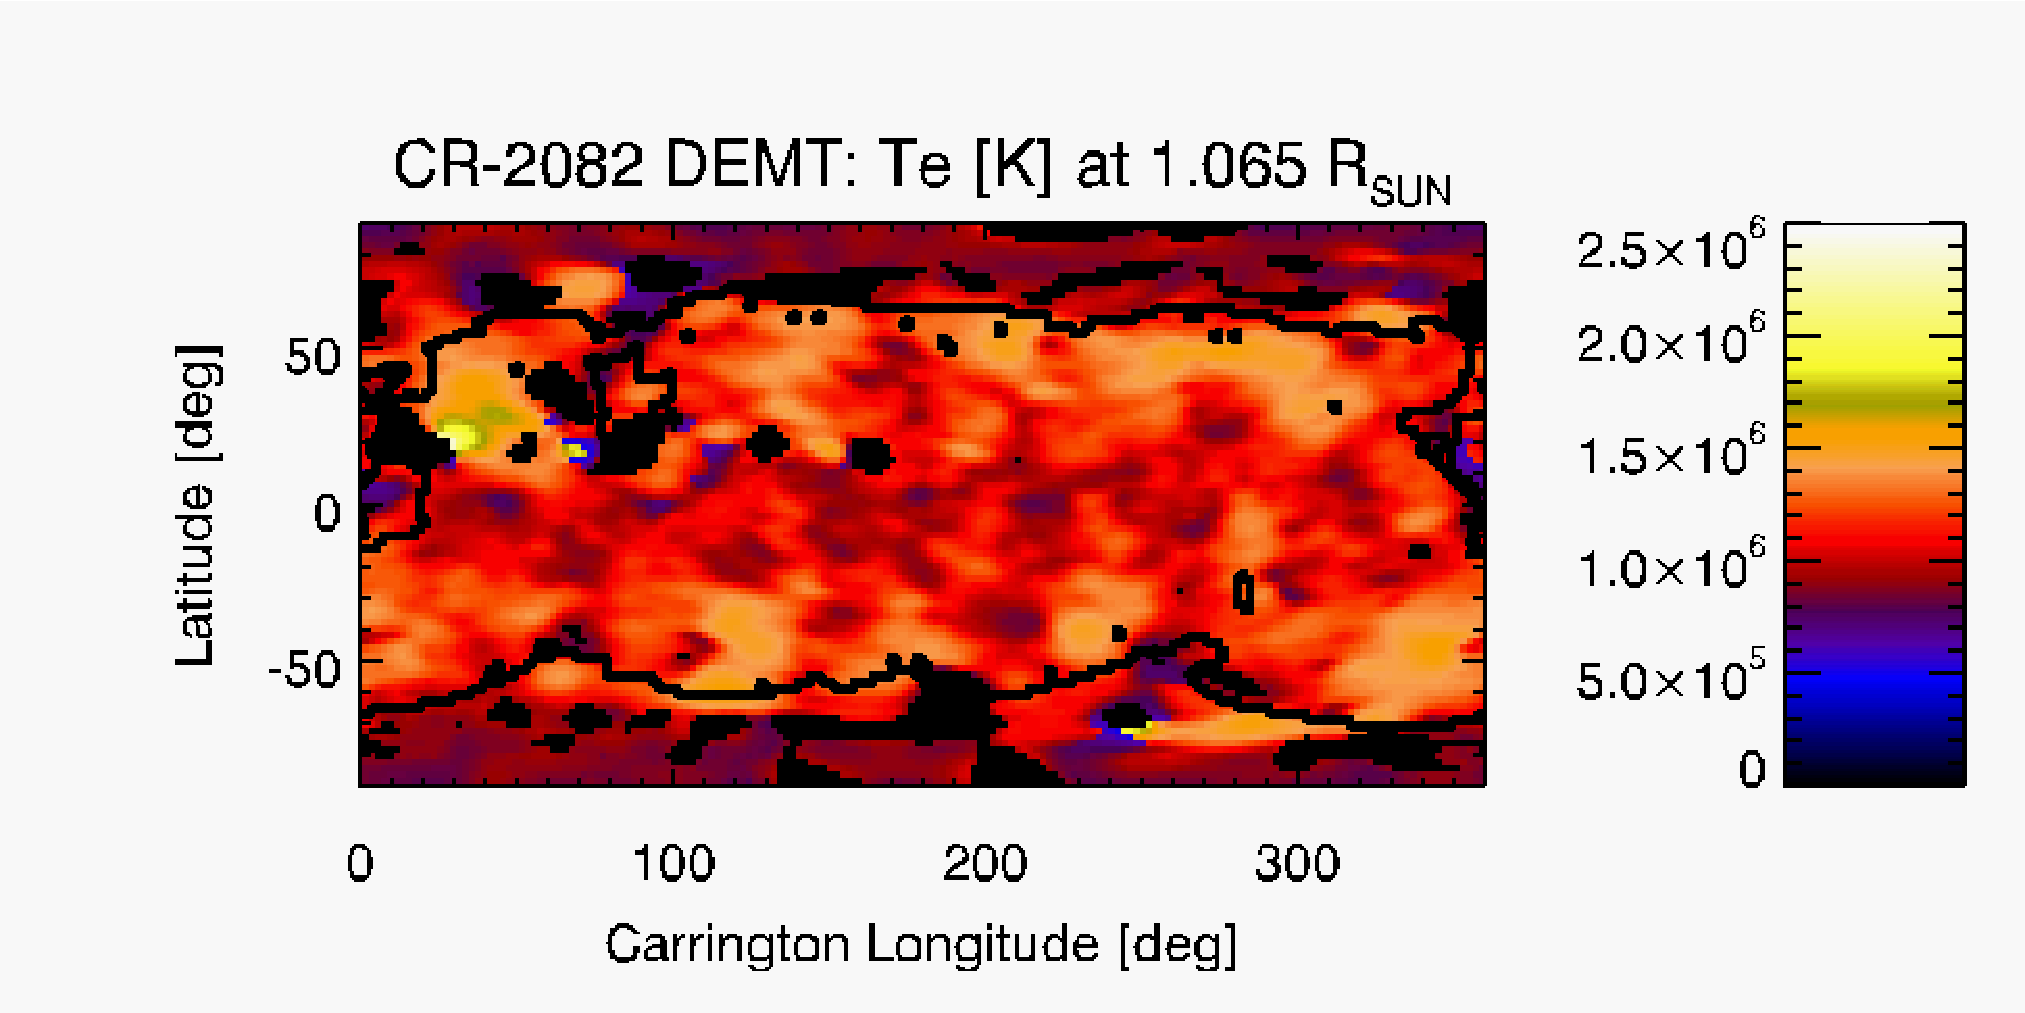
\includegraphics[width=0.495\textwidth]{figs/map_Tm_CR2082_DEMT-EUVI_behind_H1-L3523_r3d_1065_Rsun.pdf}
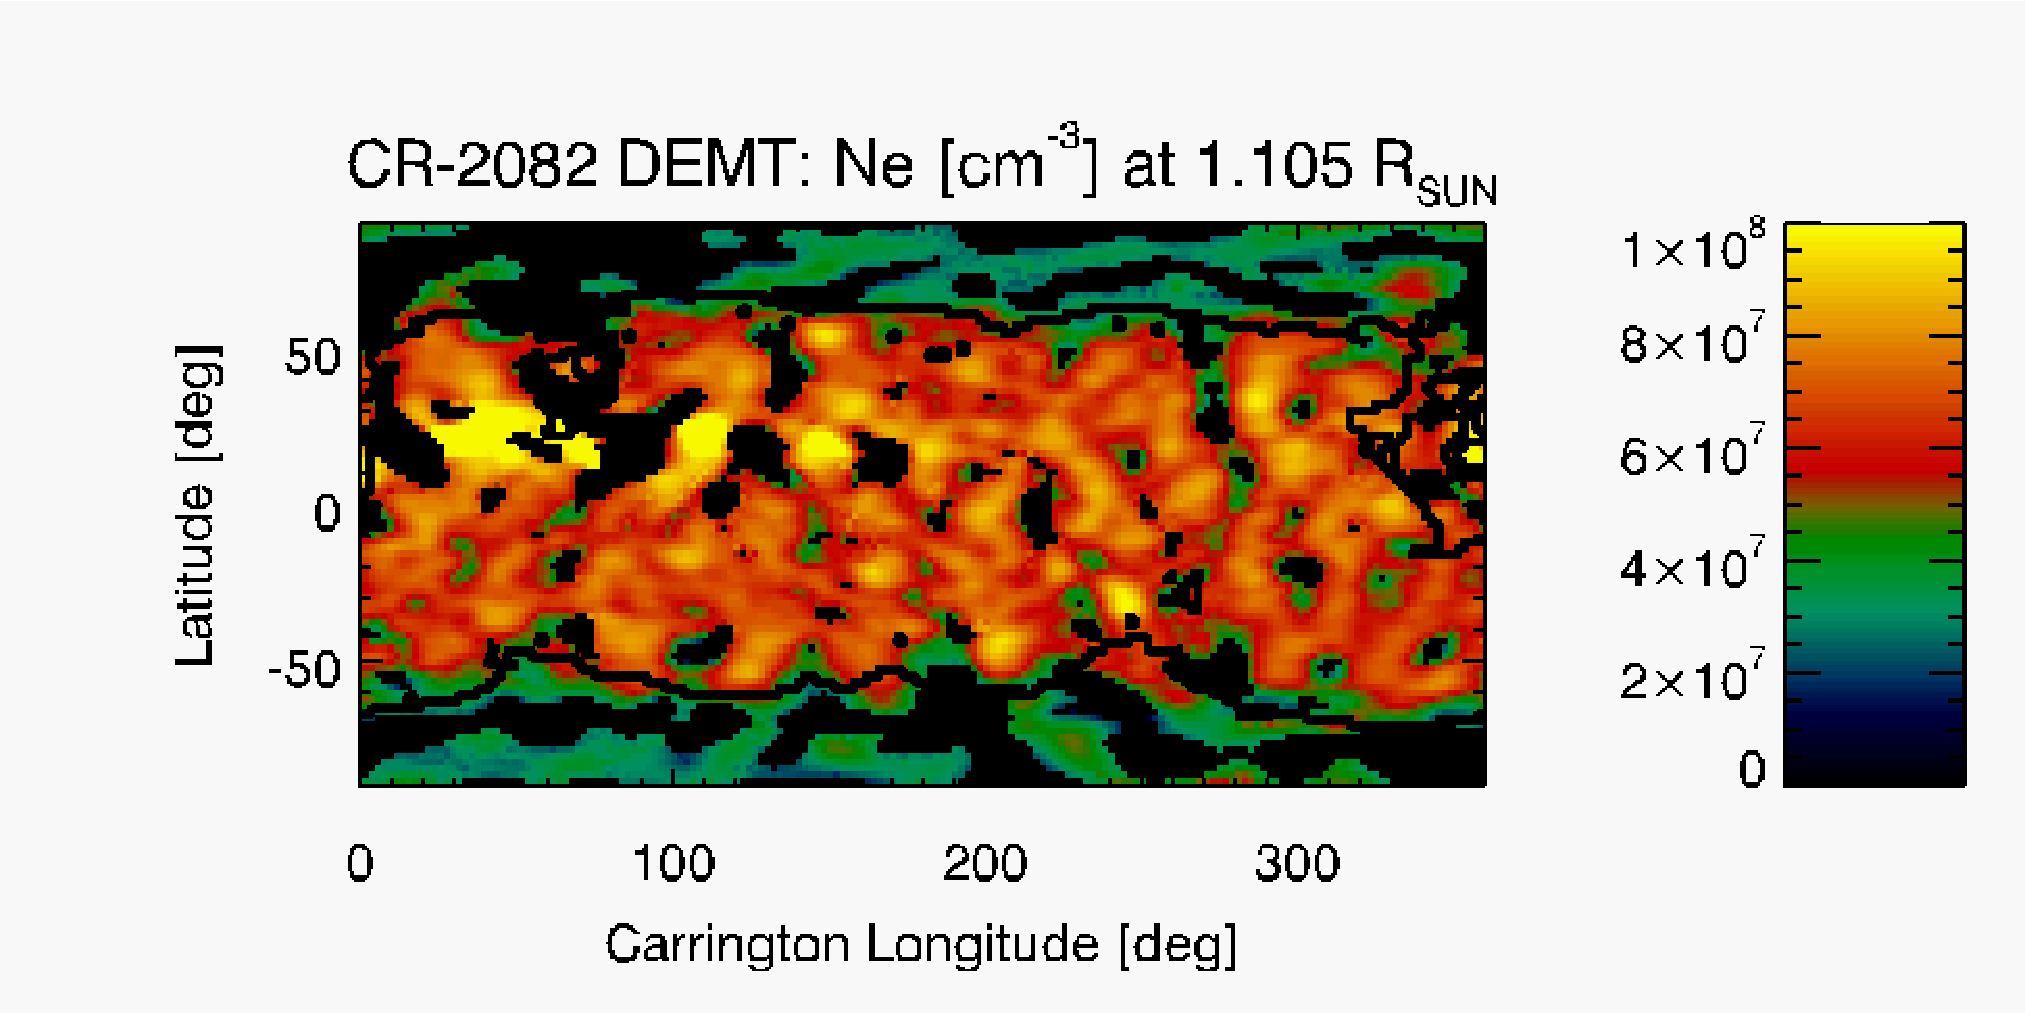
\includegraphics[width=0.495\textwidth]{figs/map_Ne_CR2082_DEMT-EUVI_behind_H1-L3523_r3d_1105_Rsun.pdf}
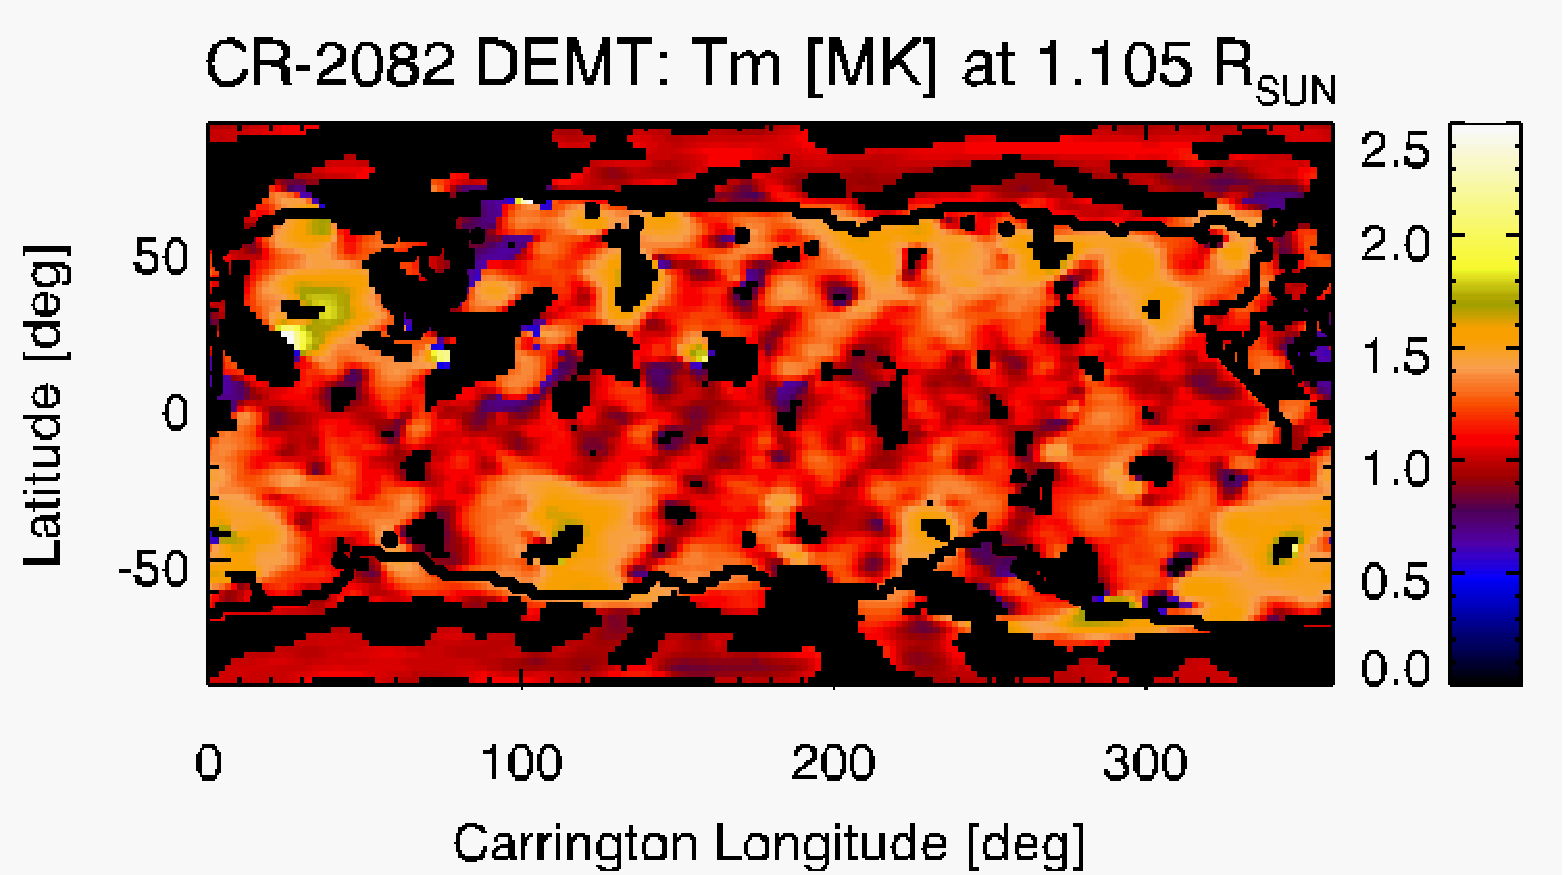
\includegraphics[width=0.495\textwidth]{figs/map_Tm_CR2082_DEMT-EUVI_behind_H1-L3523_r3d_1105_Rsun.pdf}
\caption{Carrington maps of DEMT results: $N_e$ (left panels) and $T_\textrm{m}$ (right panels) for CR-2082. Top, middle and bottom panels show the results at three heliocentric heights, $1.025$, $1.065$ and $1.105\,\mrsun$ respectively. Black voxels correspond to non-reconstructed regions (see text in Section \ref{demt_res}) and thick-black curves indicate the open/closed boundaries.}
\label{carmaps_demt_2082}
\end{center}
\end{figure}

\begin{figure}[h!]
\begin{center}
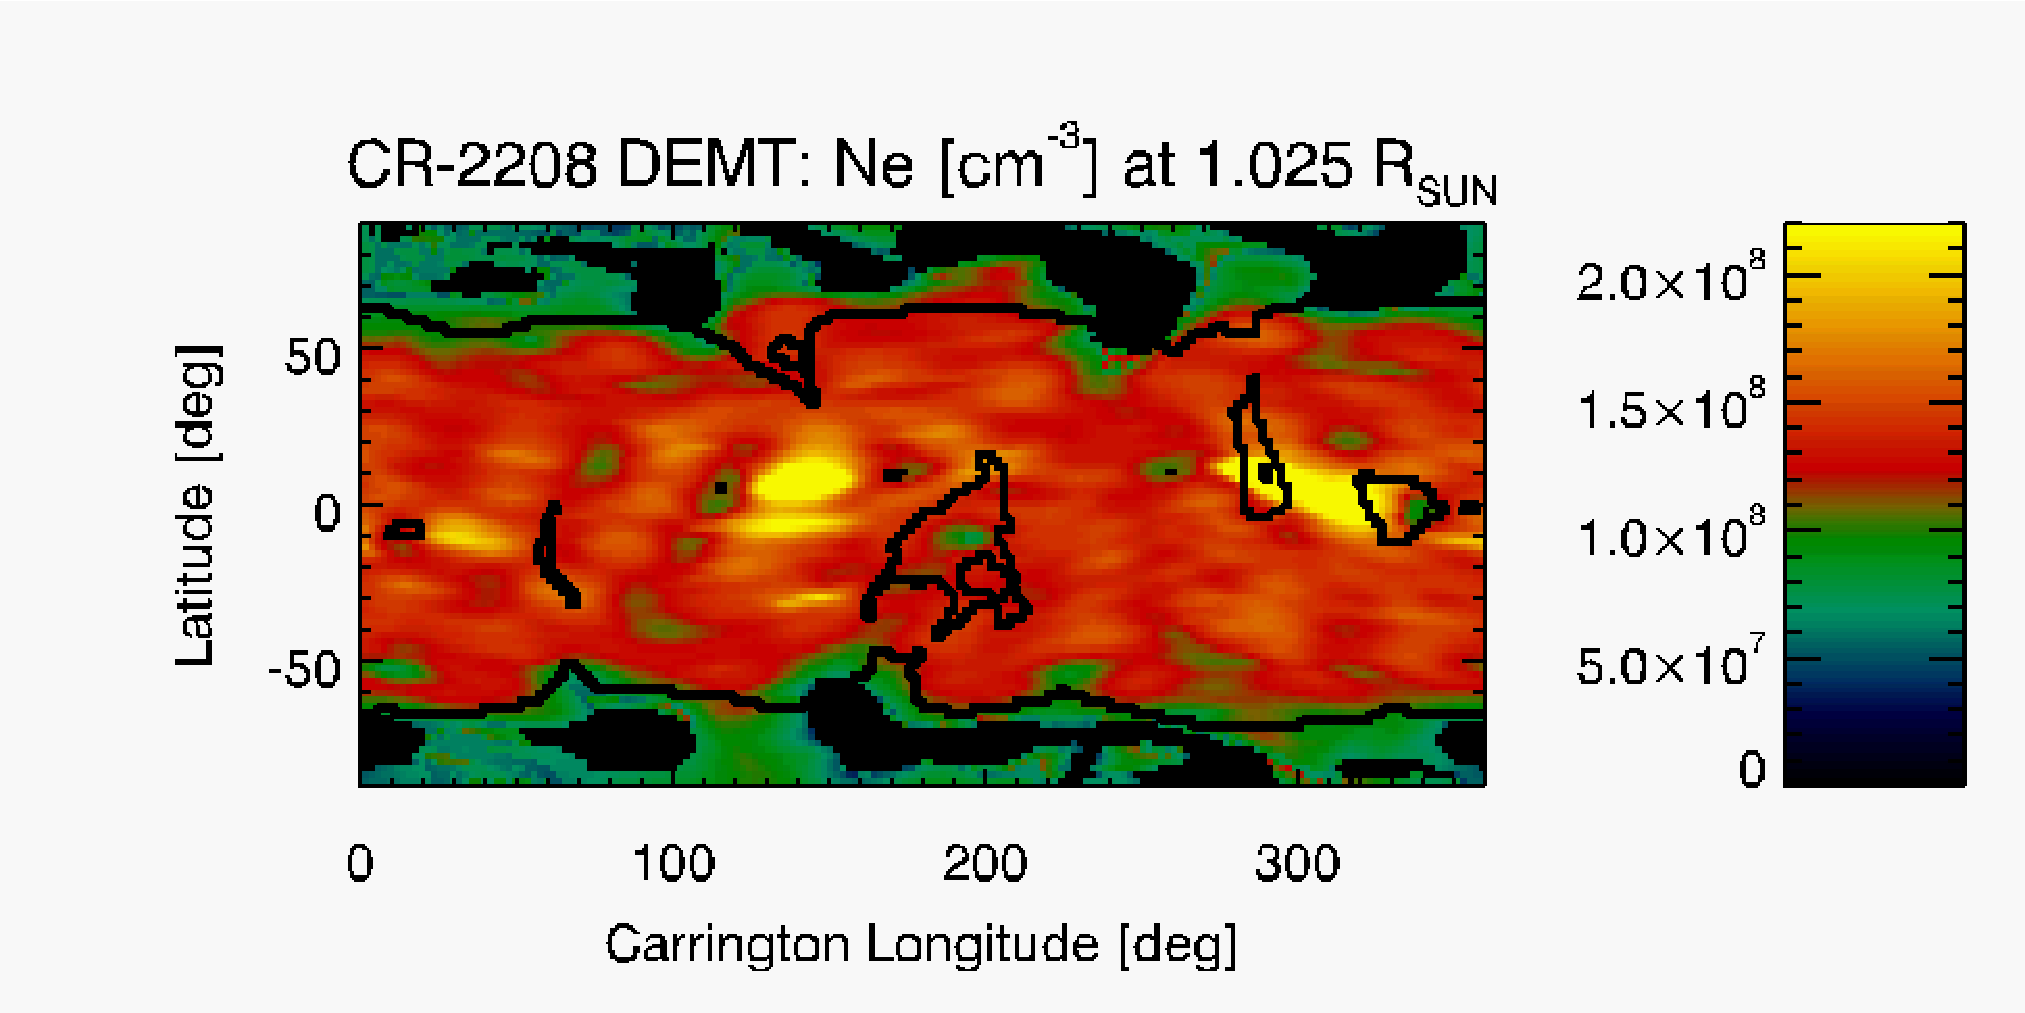
\includegraphics[width=0.495\textwidth]{figs/map_Ne_CR2208_DEMT-AIA_H1_L522_r3d_1025_Rsun.pdf}
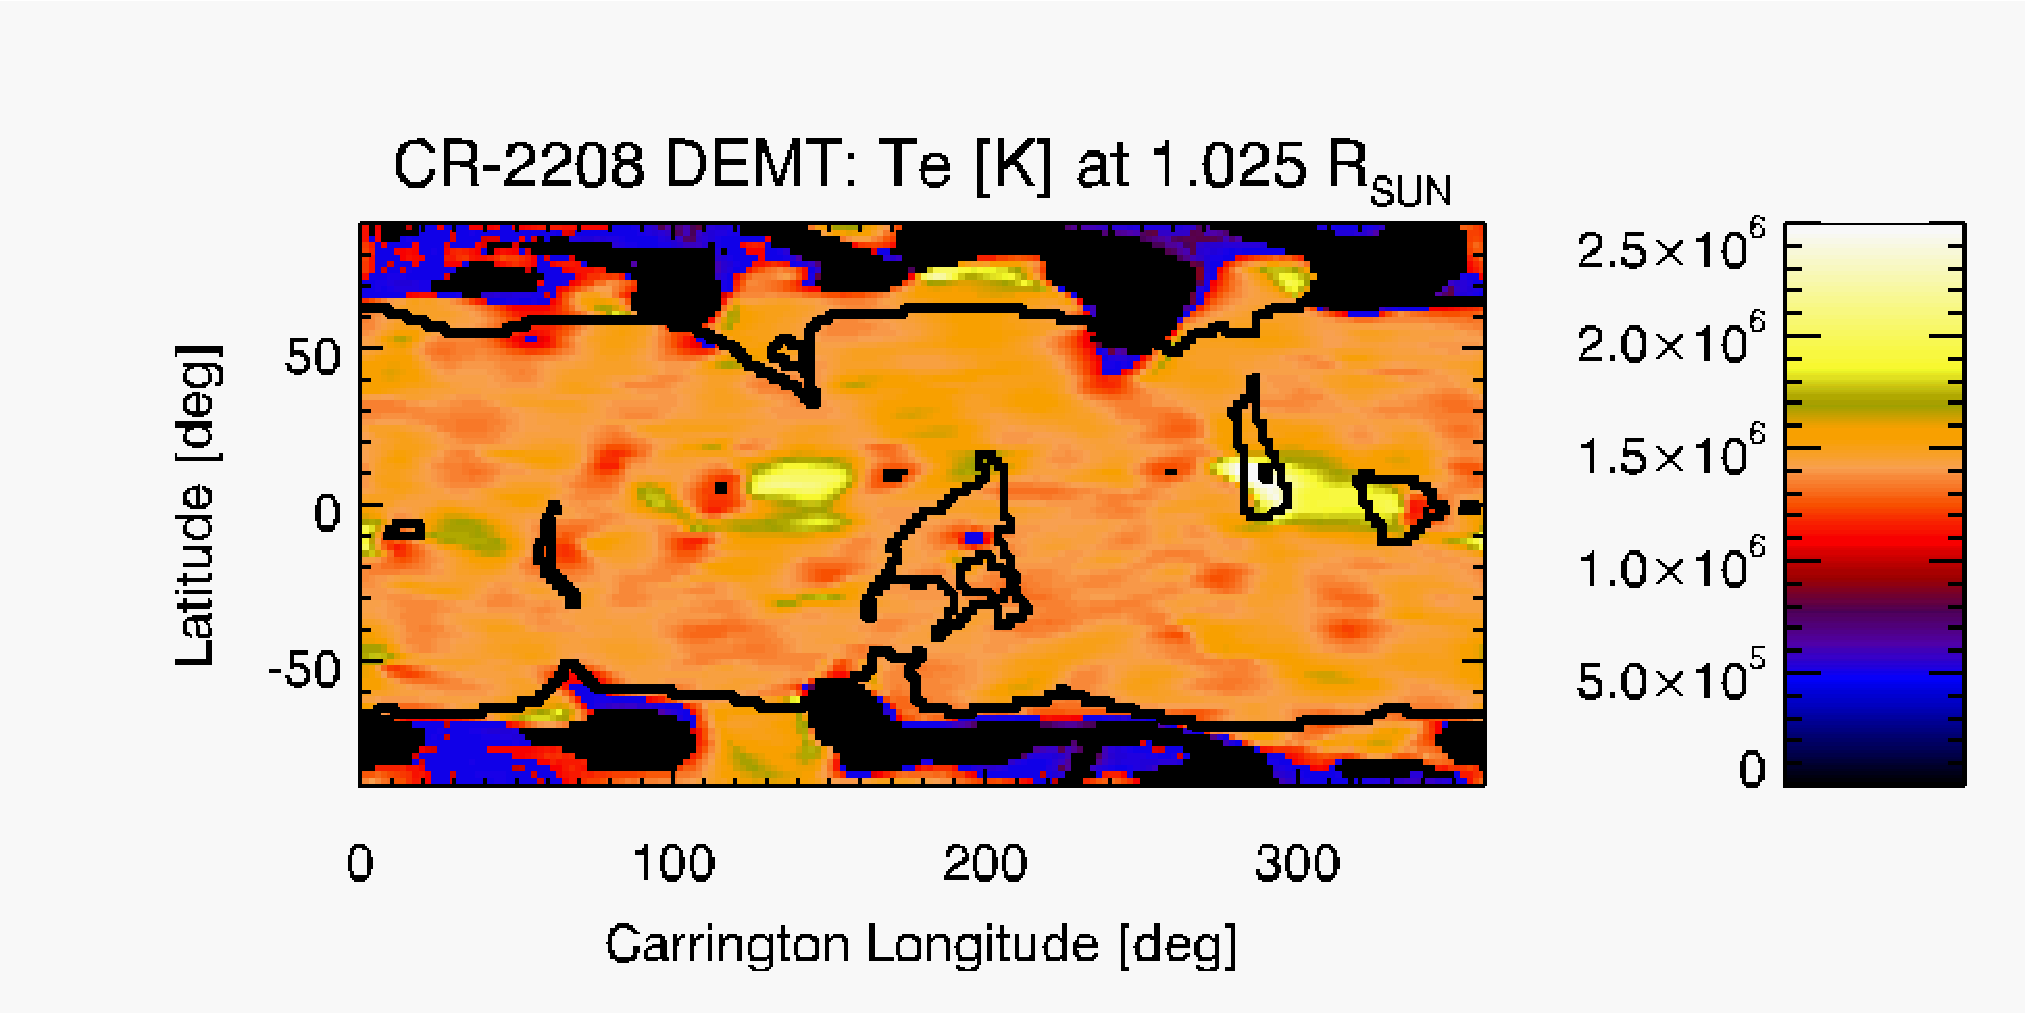
\includegraphics[width=0.495\textwidth]{figs/map_Tm_CR2208_DEMT-AIA_H1_L522_r3d_1025_Rsun.pdf}
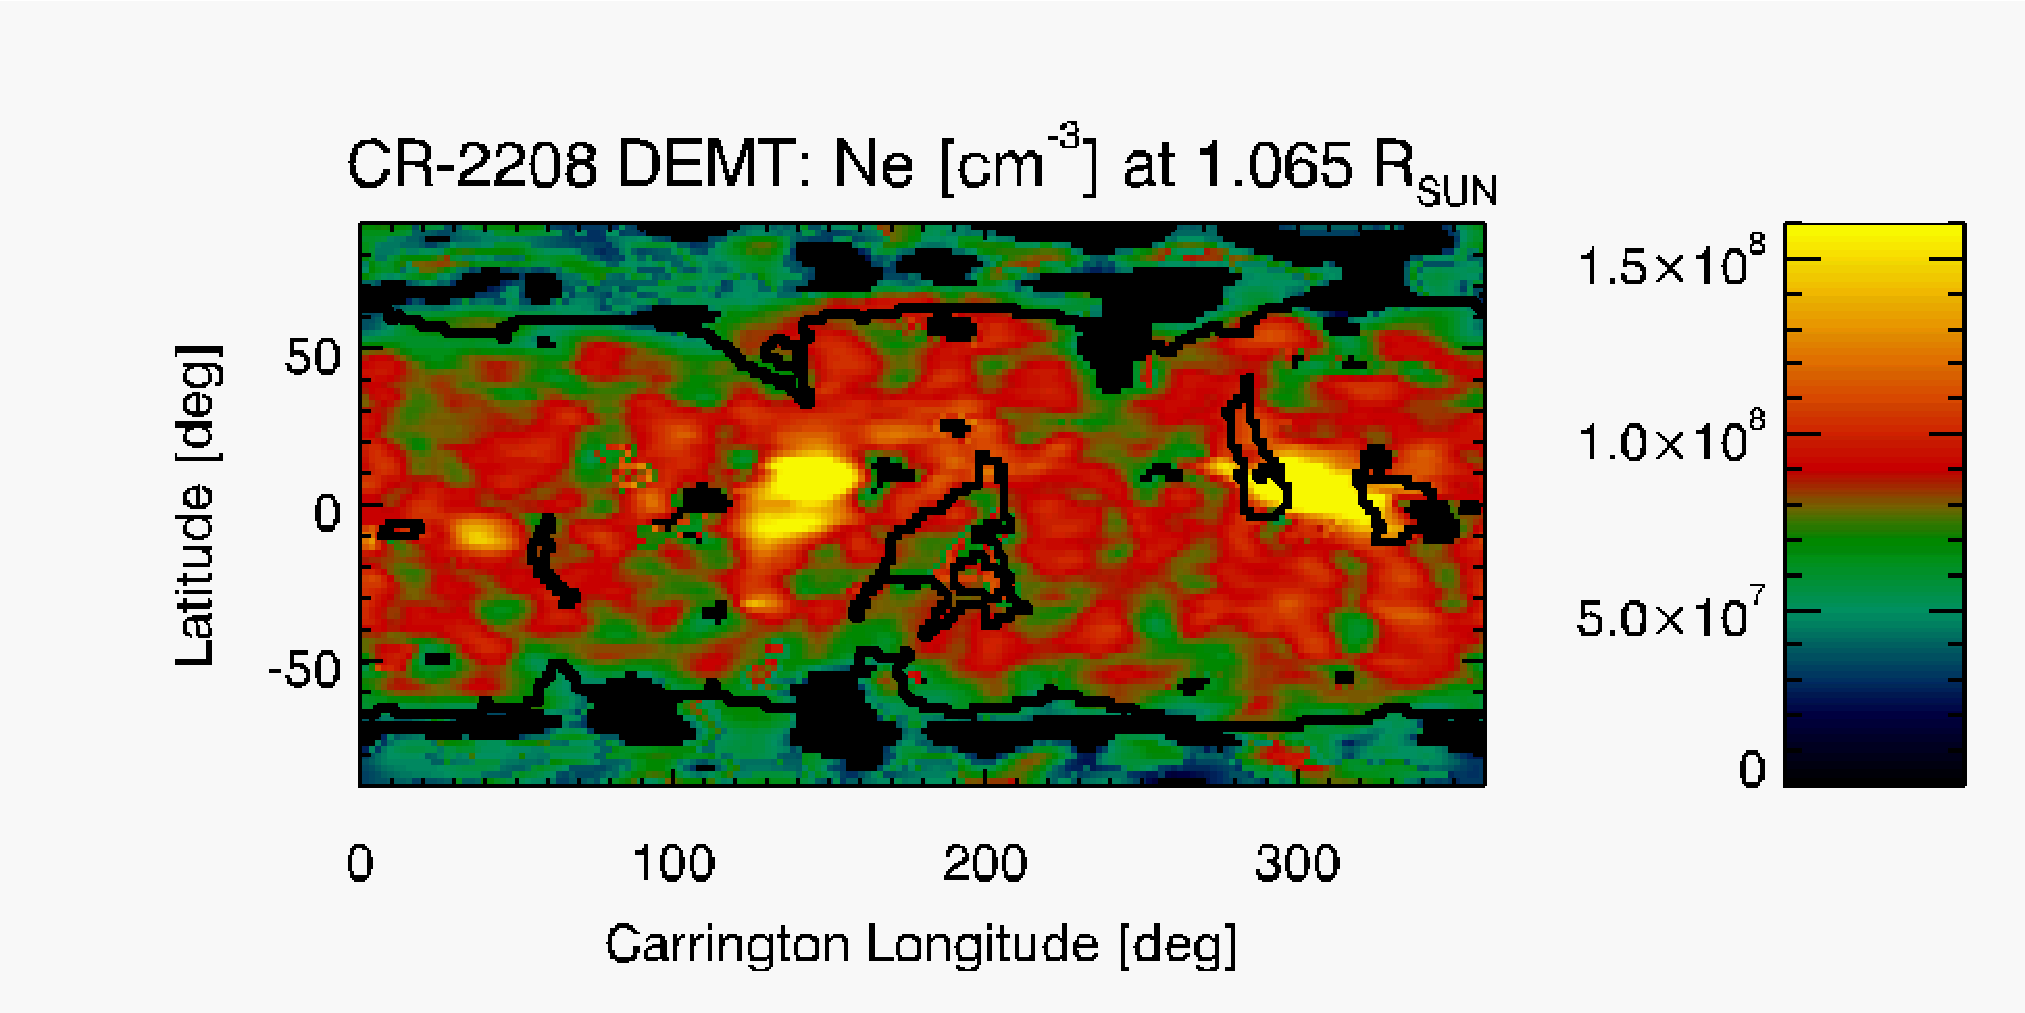
\includegraphics[width=0.495\textwidth]{figs/map_Ne_CR2208_DEMT-AIA_H1_L522_r3d_1065_Rsun.pdf}
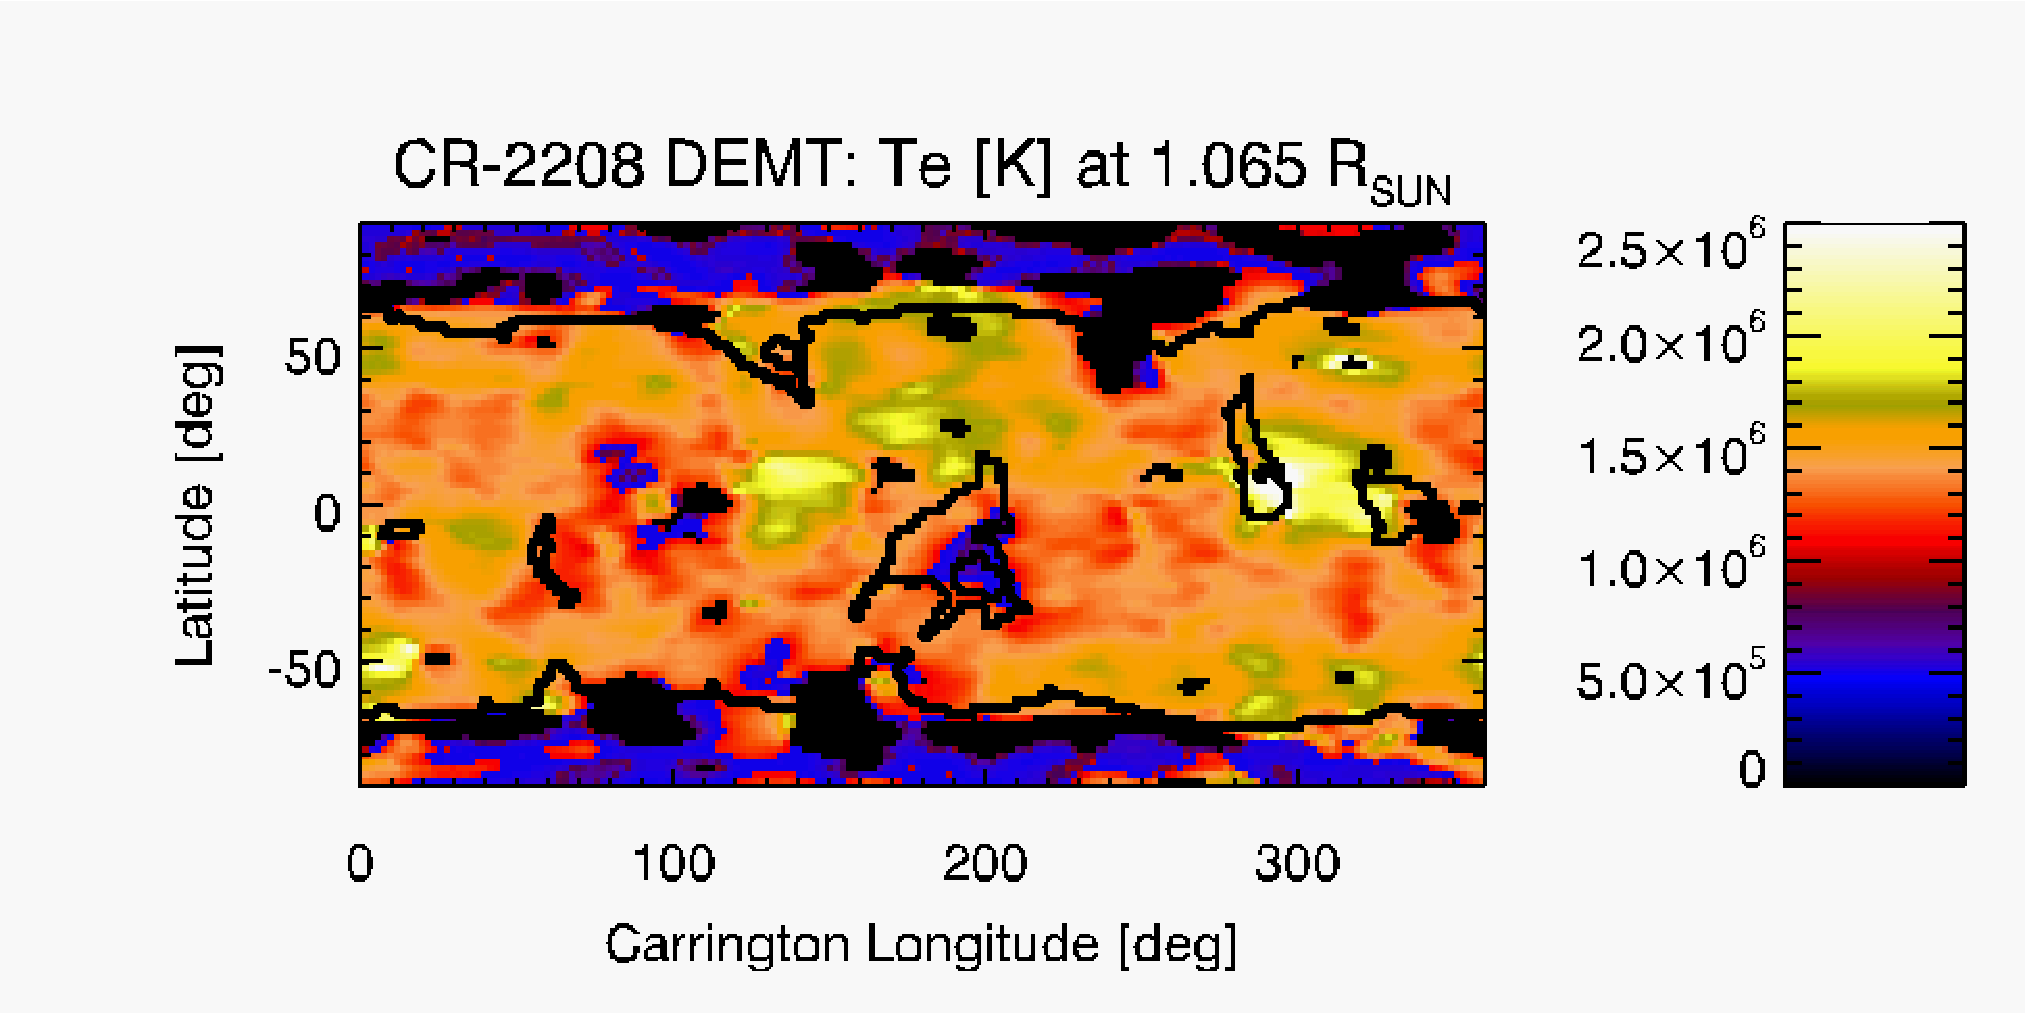
\includegraphics[width=0.495\textwidth]{figs/map_Tm_CR2208_DEMT-AIA_H1_L522_r3d_1065_Rsun.pdf}
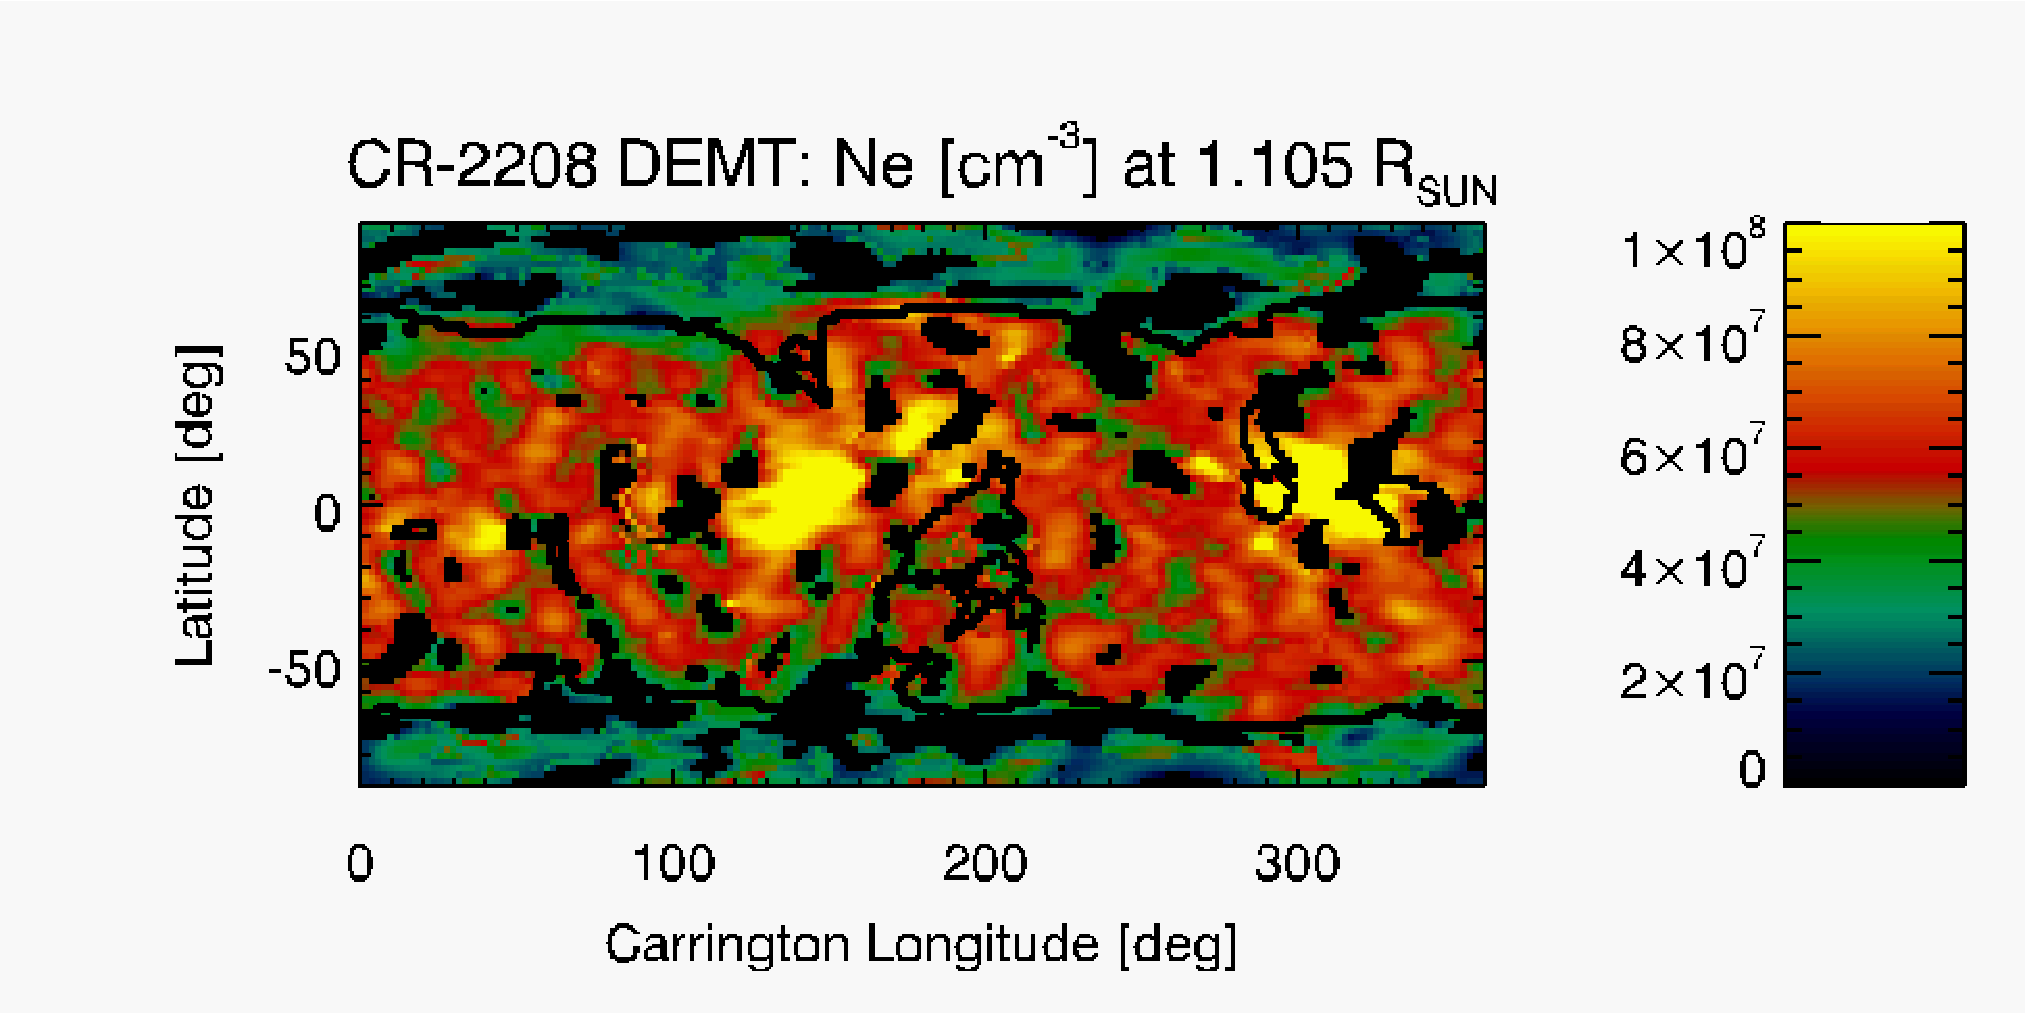
\includegraphics[width=0.495\textwidth]{figs/map_Ne_CR2208_DEMT-AIA_H1_L522_r3d_1105_Rsun.pdf}
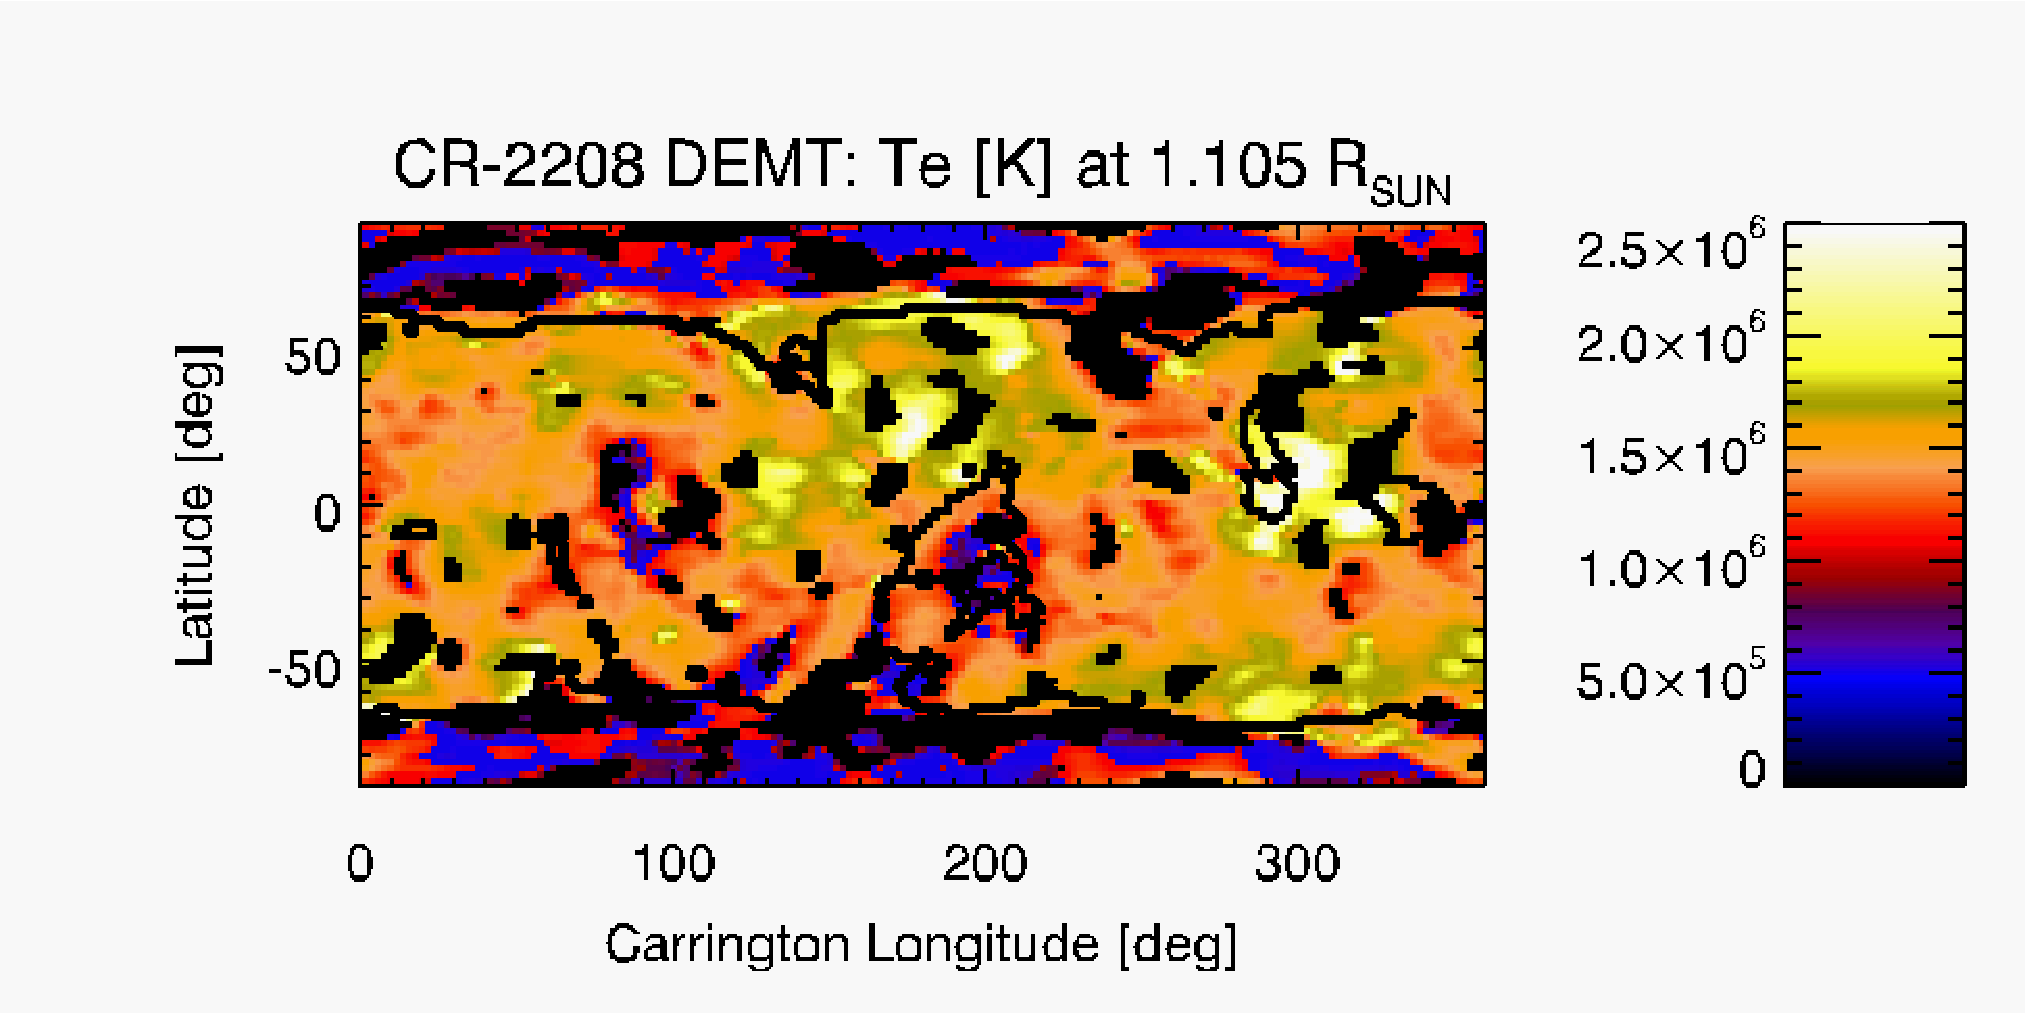
\includegraphics[width=0.495\textwidth]{figs/map_Tm_CR2208_DEMT-AIA_H1_L522_r3d_1105_Rsun.pdf}
\caption{Same as Figure \ref{carmaps_demt_2082} but for CR-2208.}
\label{carmaps_demt_2208}
\end{center}
\end{figure}

\textcolor{red}{
*Para las piernas trazadas que cumplen  |pearson de temp| > 0.5 se calcularon los gradientes de temp que cumplen test de hipotesis. Estos gradientes se muestran en la Figura \ref{gradientes} para las 3 regiones definidas para ambas rotaciones. Esto muestra up y down loops.
OBS: esto da pie a hablar y proponer mejoras en la conversion de modos de alfven. citar paper fede.
%*Como el modelo awsom no presenta down loops, se selecciona de ahora en mas los loops con pearson de temp > 0.5
}
%\begin{figure}[h!]
%\begin{center}
%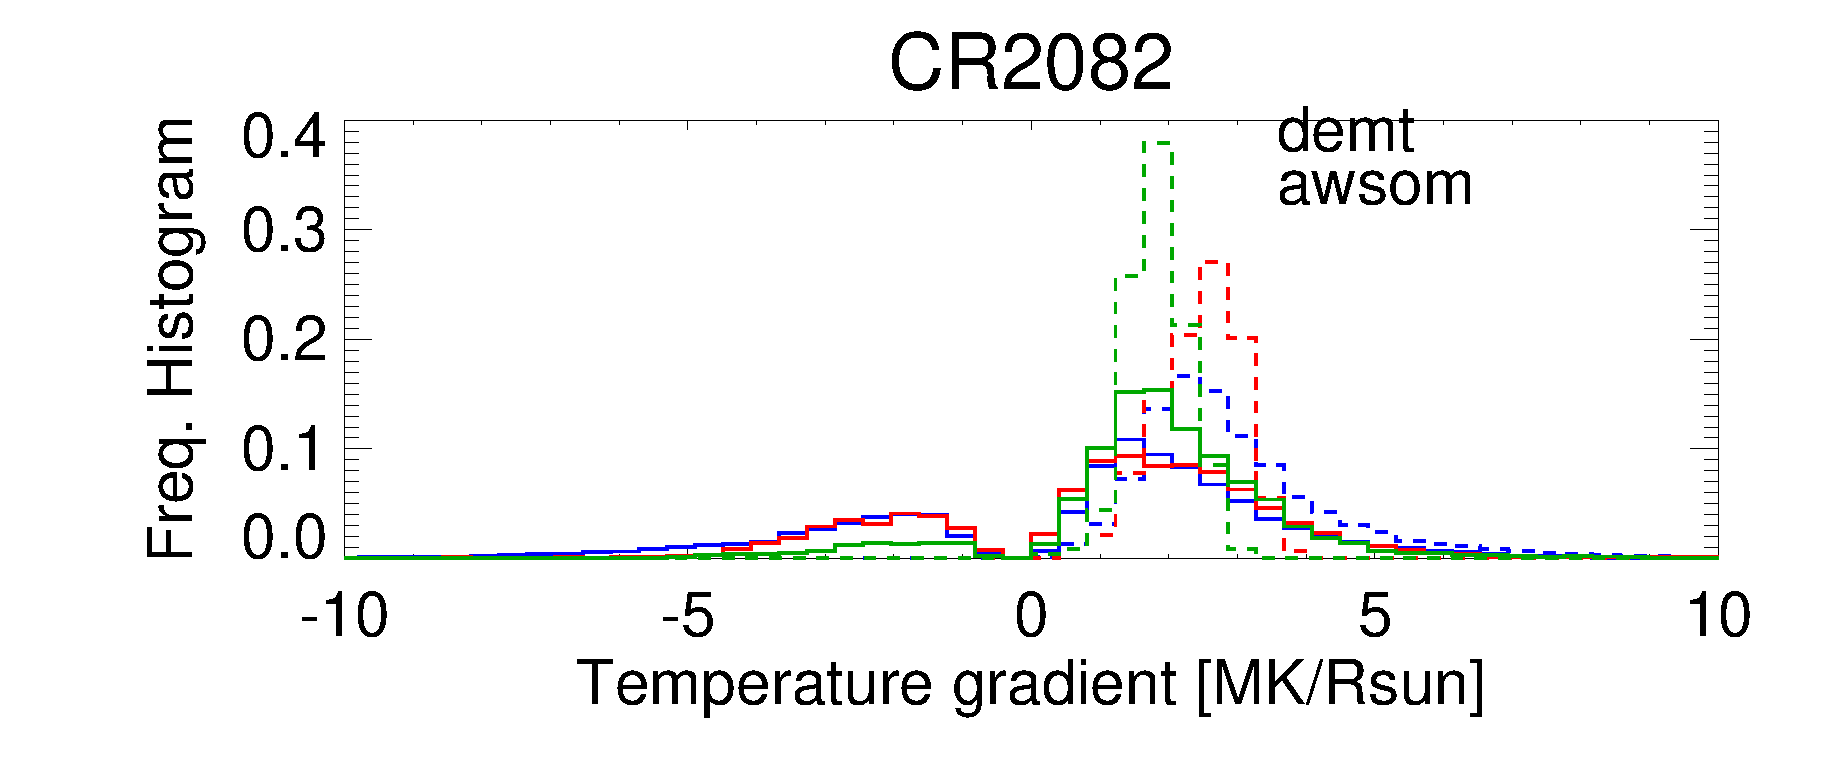
\includegraphics[width=0.495\textwidth,clip=]{figs/histo_cr2082_updowntriple_gradt.eps}
%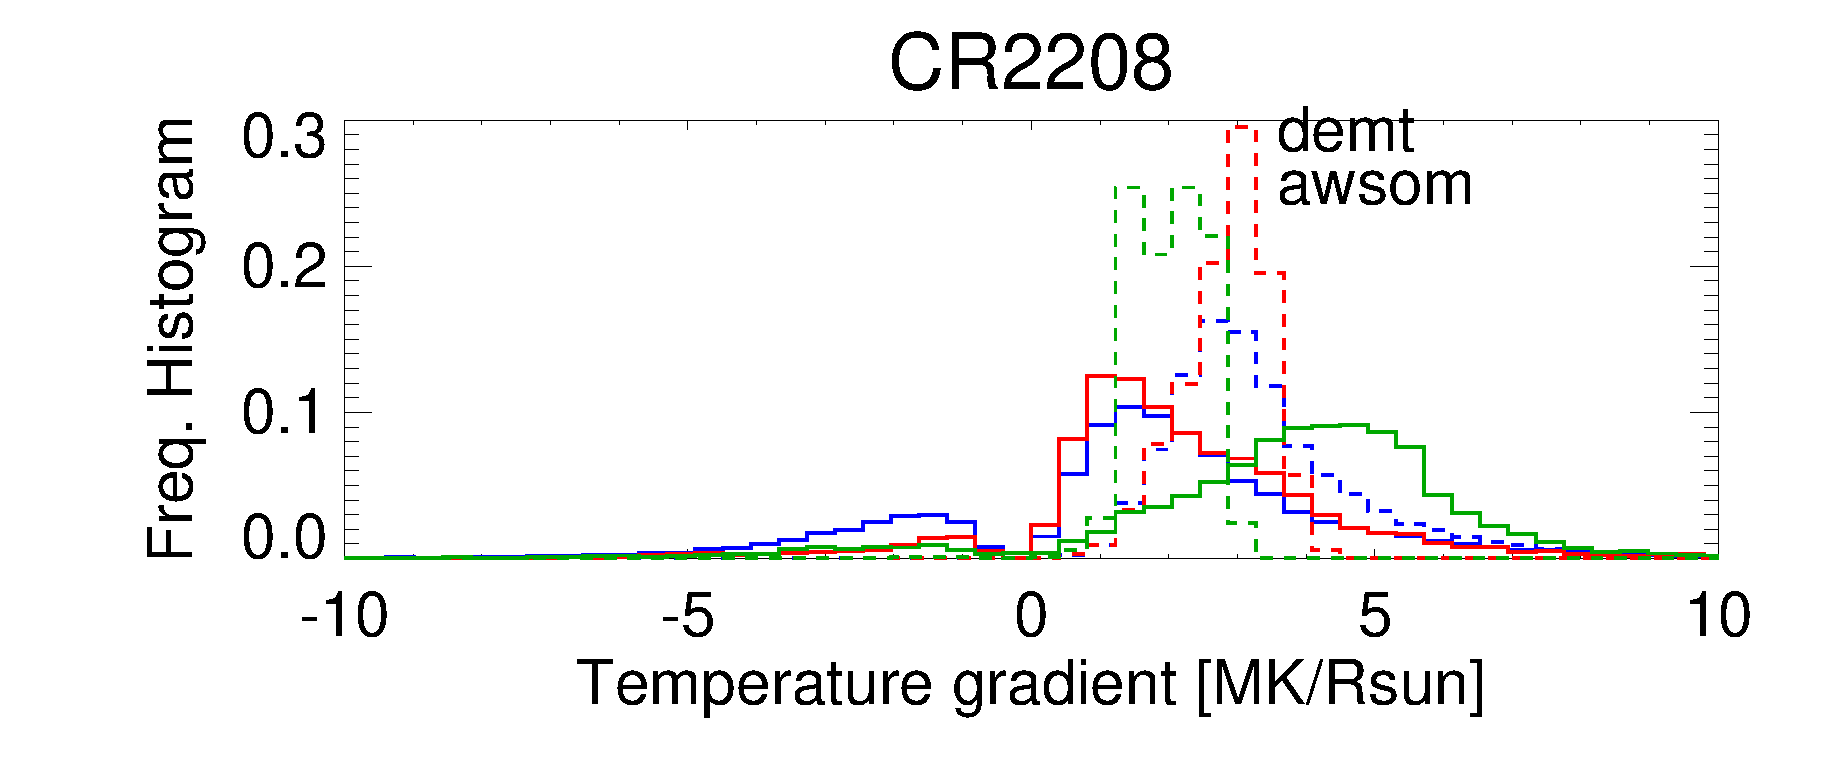
\includegraphics[width=0.495\textwidth,clip=]{figs/histo_cr2208_updowntriple_gradt.eps}
%\caption{Frequency histogram of the temperature radial gradient of along each leg of type I (in blue), type II %(in red) and type III (in green) meeting the criteria listed in Section \ref{trace} for CR-2082 (left panel) and CR-2208 (right panel). In solid lines DEMT traced data and in dashed lines AWSoM data.}
%\label{gradientes}
%\end{center}
%\end{figure} 

\textcolor{red}{
For the two analyzed rotations, Figure \ref{rpoint_demt} shows the latitudinal-longitudinal location of all field lines that meet the criteria listed in Section \ref{trace} at $1.105\,\mrsun$.
}

\begin{figure}[h!]
\begin{center}
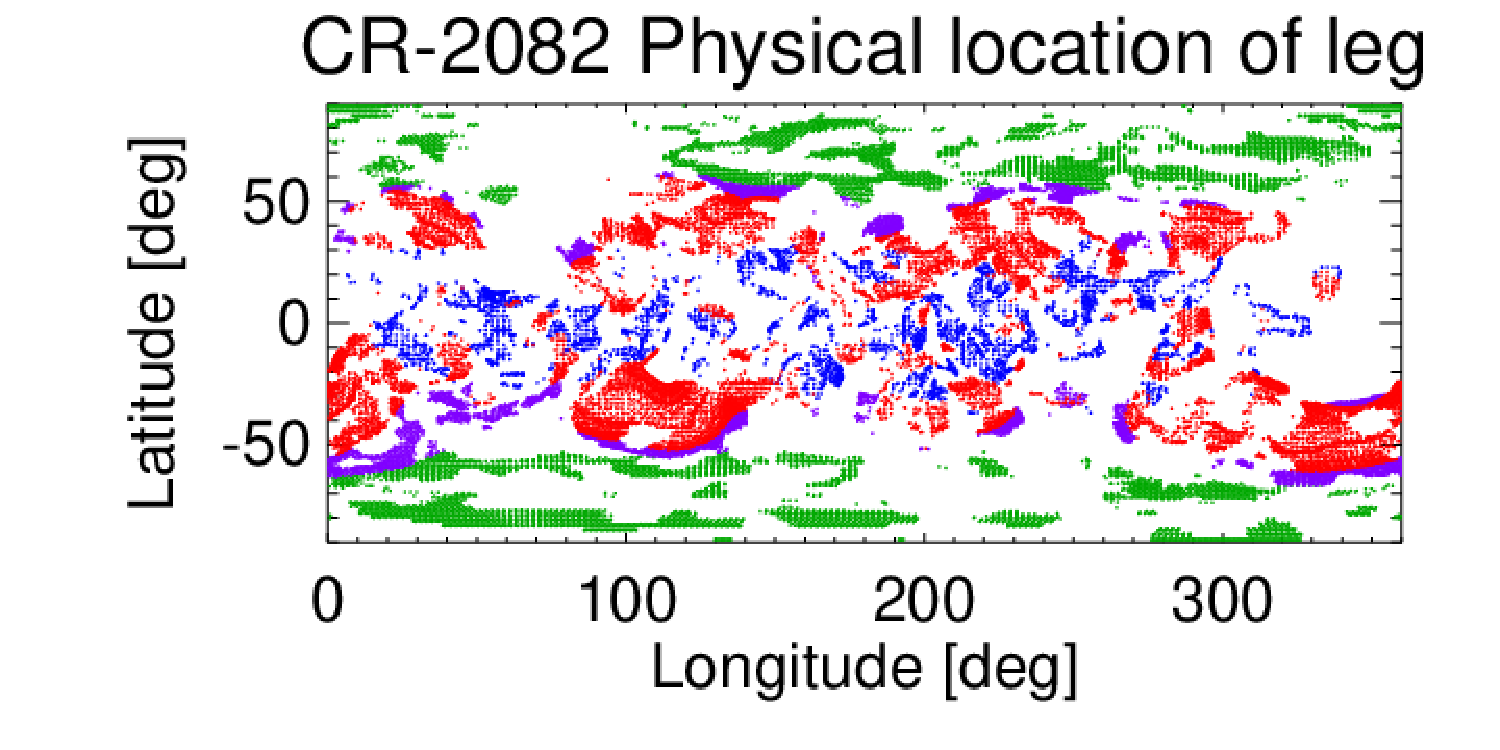
\includegraphics[width=0.495\textwidth,clip=]{figs/Highpoint_2082_demt_paper_cr2082_full_Rpoint-map.eps}
%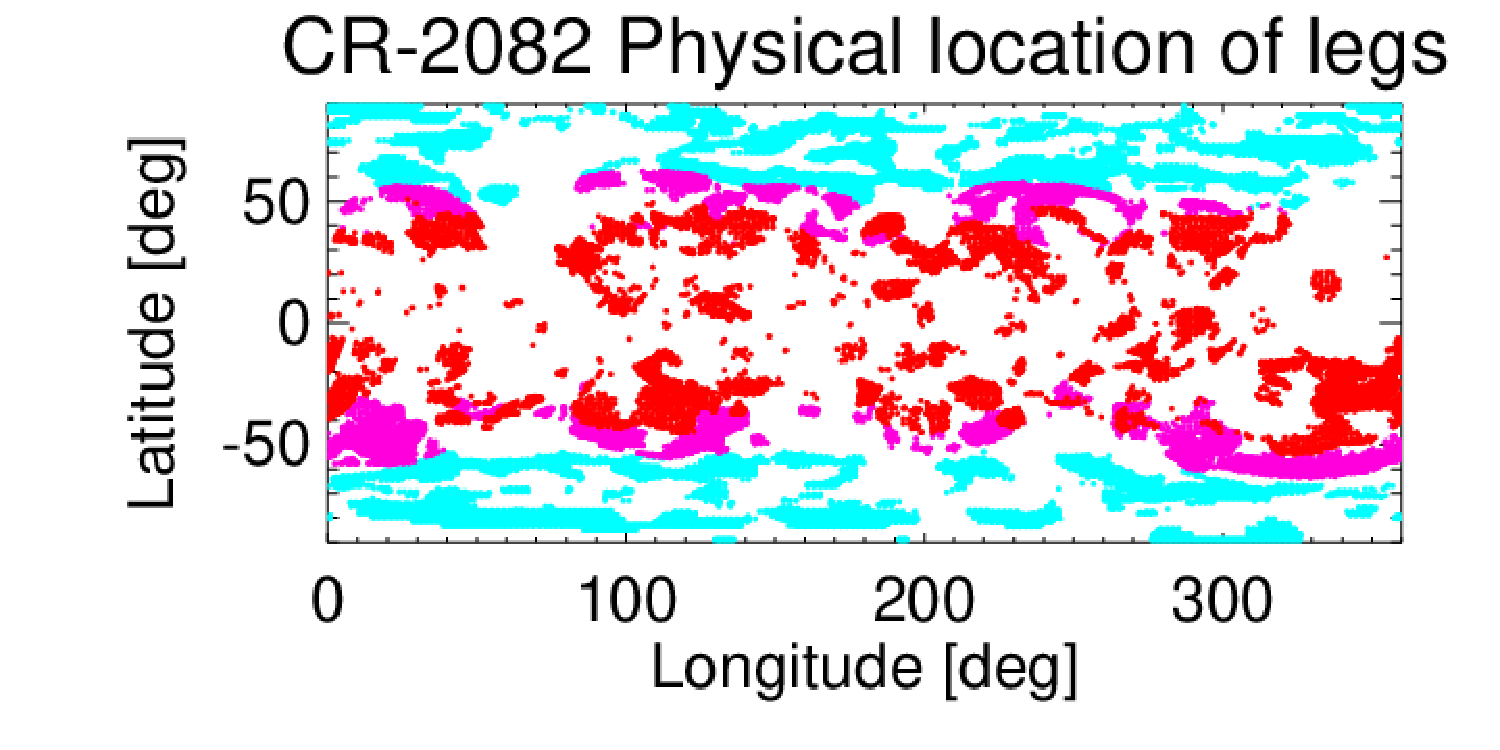
\includegraphics[width=0.495\textwidth,clip=]{figs/Highpoint_2082_demt_paper_cr2082_up_Rpoint-map.eps}
%\includegraphics[width=0.495\textwidth,clip=]{Highpoint_2082_awsom_paper_Rpoint-map.eps}
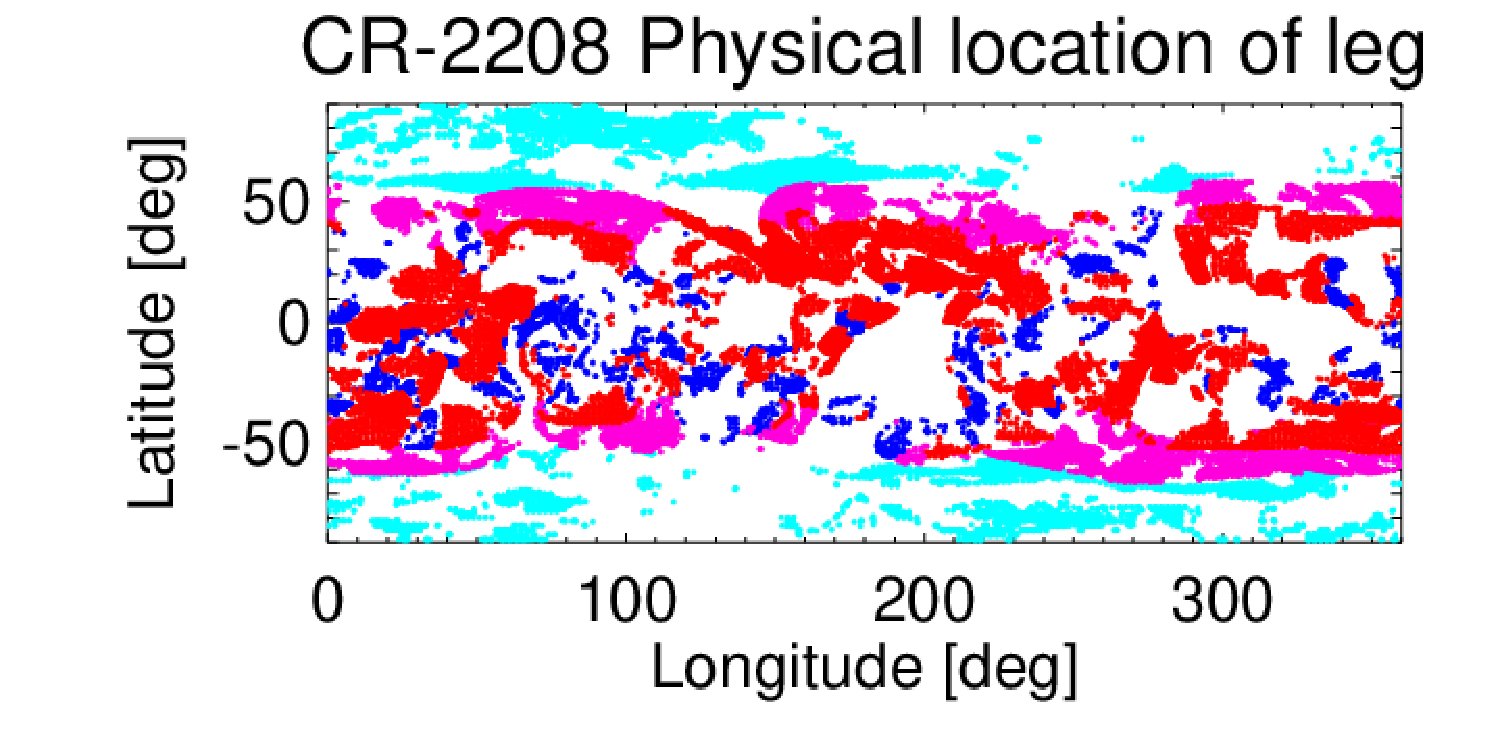
\includegraphics[width=0.495\textwidth,clip=]{figs/Highpoint_2208_demt_paper_cr2208_full_Rpoint-map.eps}
%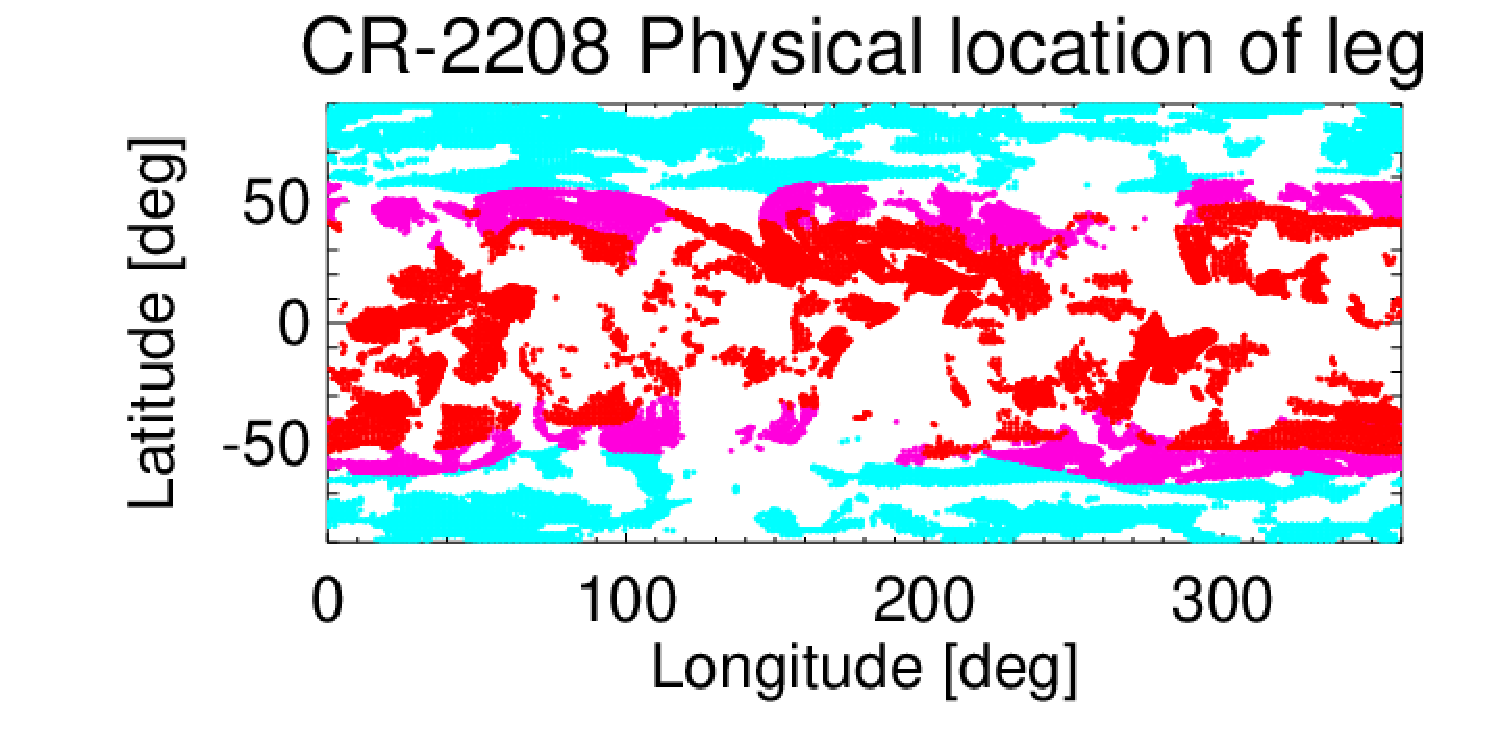
\includegraphics[width=0.495\textwidth,clip=]{figs/Highpoint_2208_demt_paper_cr2208_up_Rpoint-map.eps}
%\includegraphics[width=0.495\textwidth,clip=]{Highpoint_2208_awsom_paper_Rpoint-map.eps}
\caption{Latitude-longitude location of each leg of type 0 (in cyan), type I (in blue), type II (in red) and type III (in green) at $1.105\,\mrsun$ for CR-2082 (left panel) and CR-2208 (right panel). See Section \ref{trace} for a definition of the different types of legs.}
\label{rpoint_demt}
\end{center}
\end{figure} 

\begin{figure}[h!]
\begin{center}
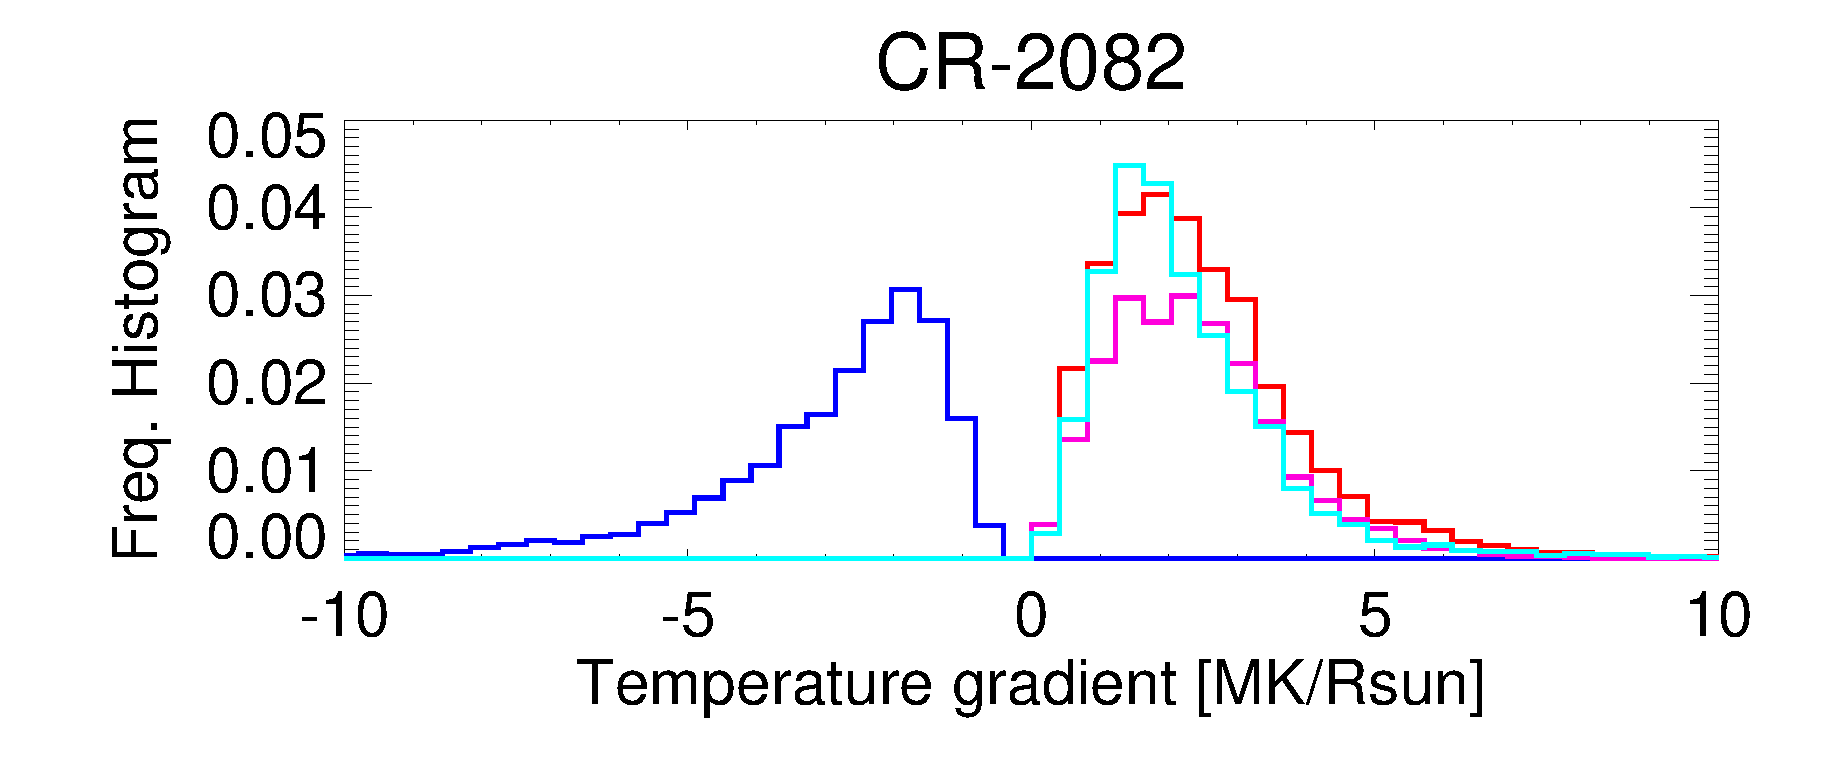
\includegraphics[width=0.495\textwidth,clip=]{figs/histo_cr2082_fulltriple_gradt.eps}
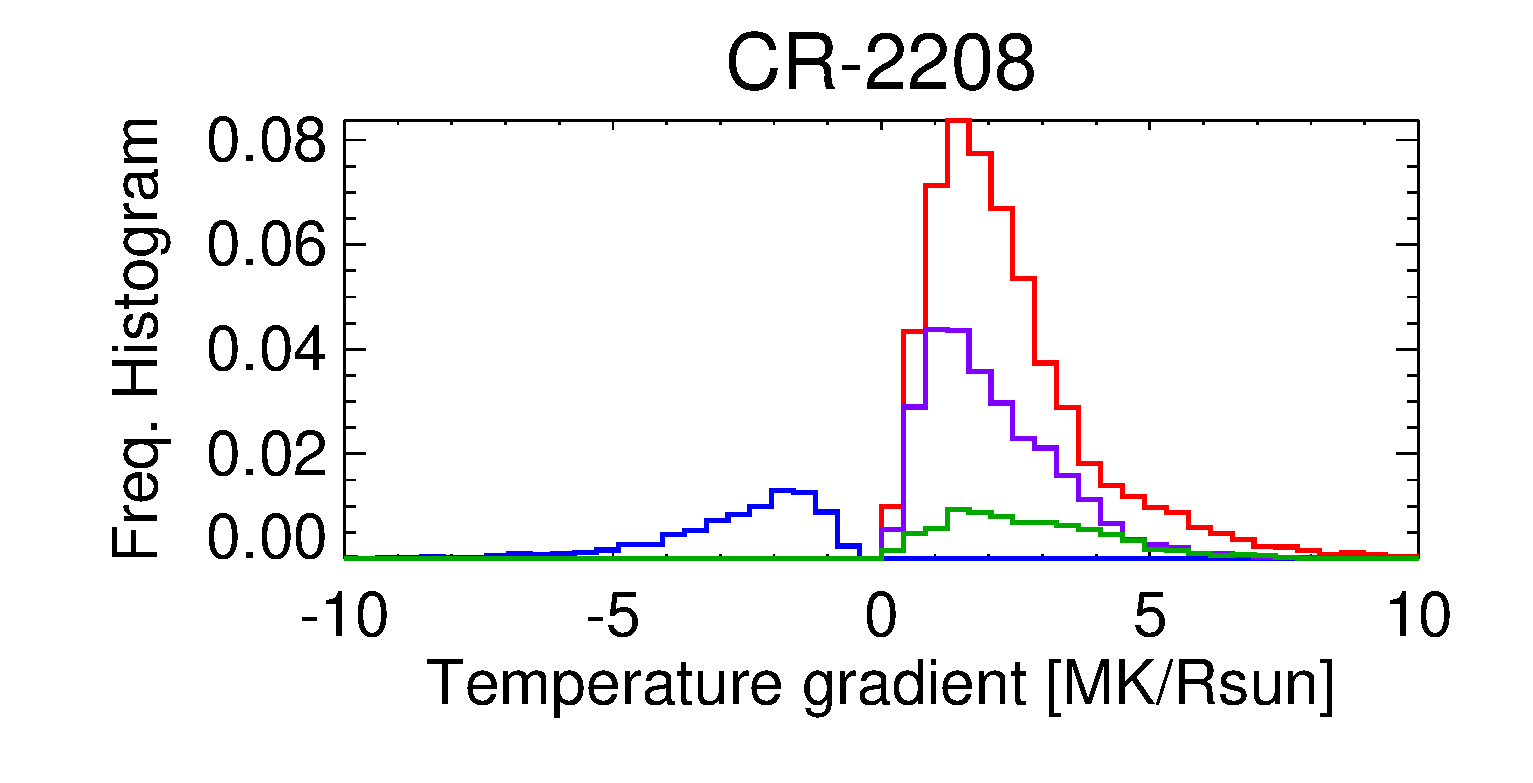
\includegraphics[width=0.495\textwidth,clip=]{figs/histo_cr2208_fulltriple_gradt.eps}
\caption{Frequency histograms of the temperature radial gradient for the different types of legs shown in Figure \ref{rpoint_demt} (same colour code) for CR-2082 (left panel) and CR-2208 (right panel).}
\label{gradt_demt}
\end{center}
\end{figure} 

\begin{figure}[h!]
\begin{center}
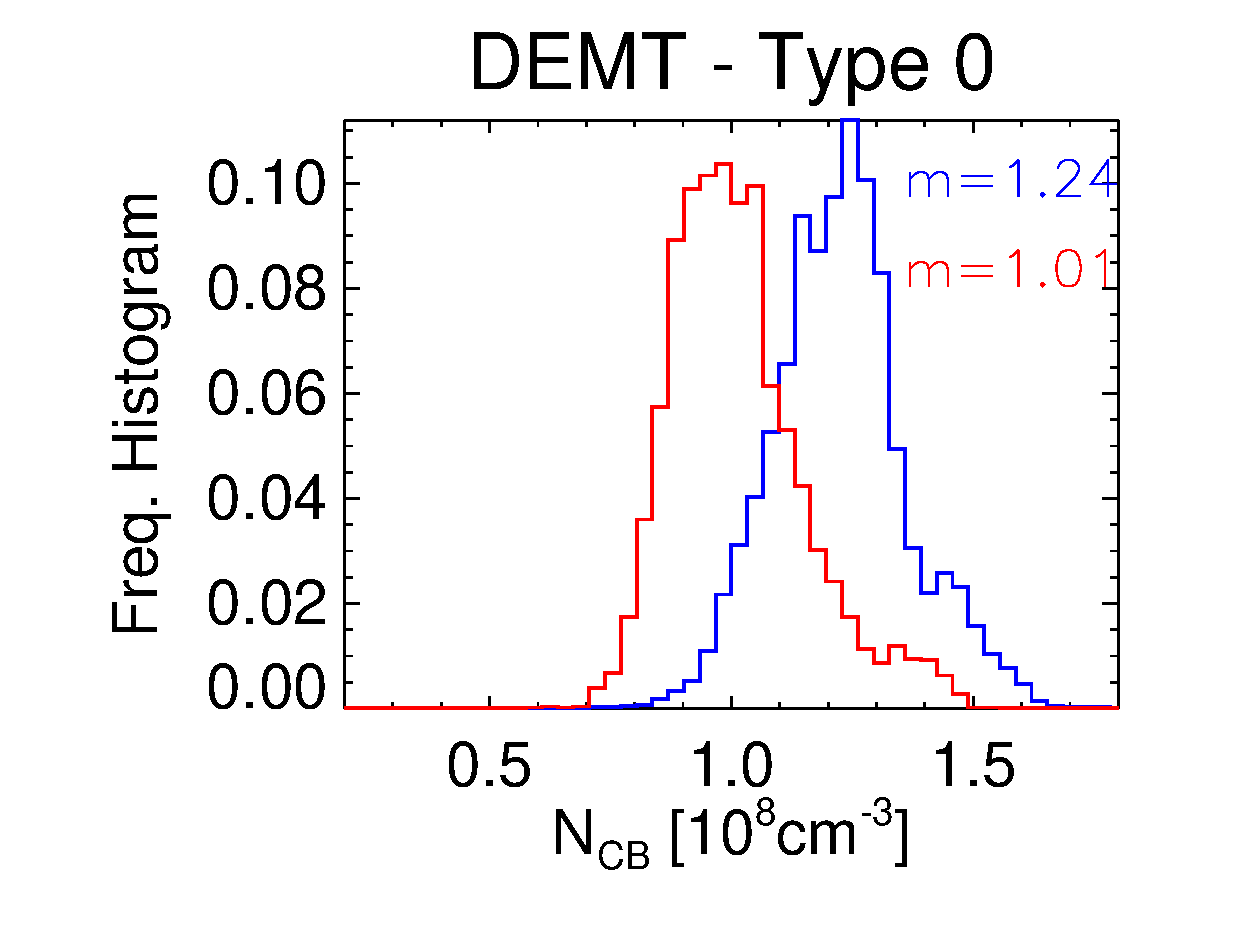
\includegraphics[width=0.31\textwidth,clip=]{figs/histo_2082_2208_fulldemt_streamer_down_ne_1055.eps}
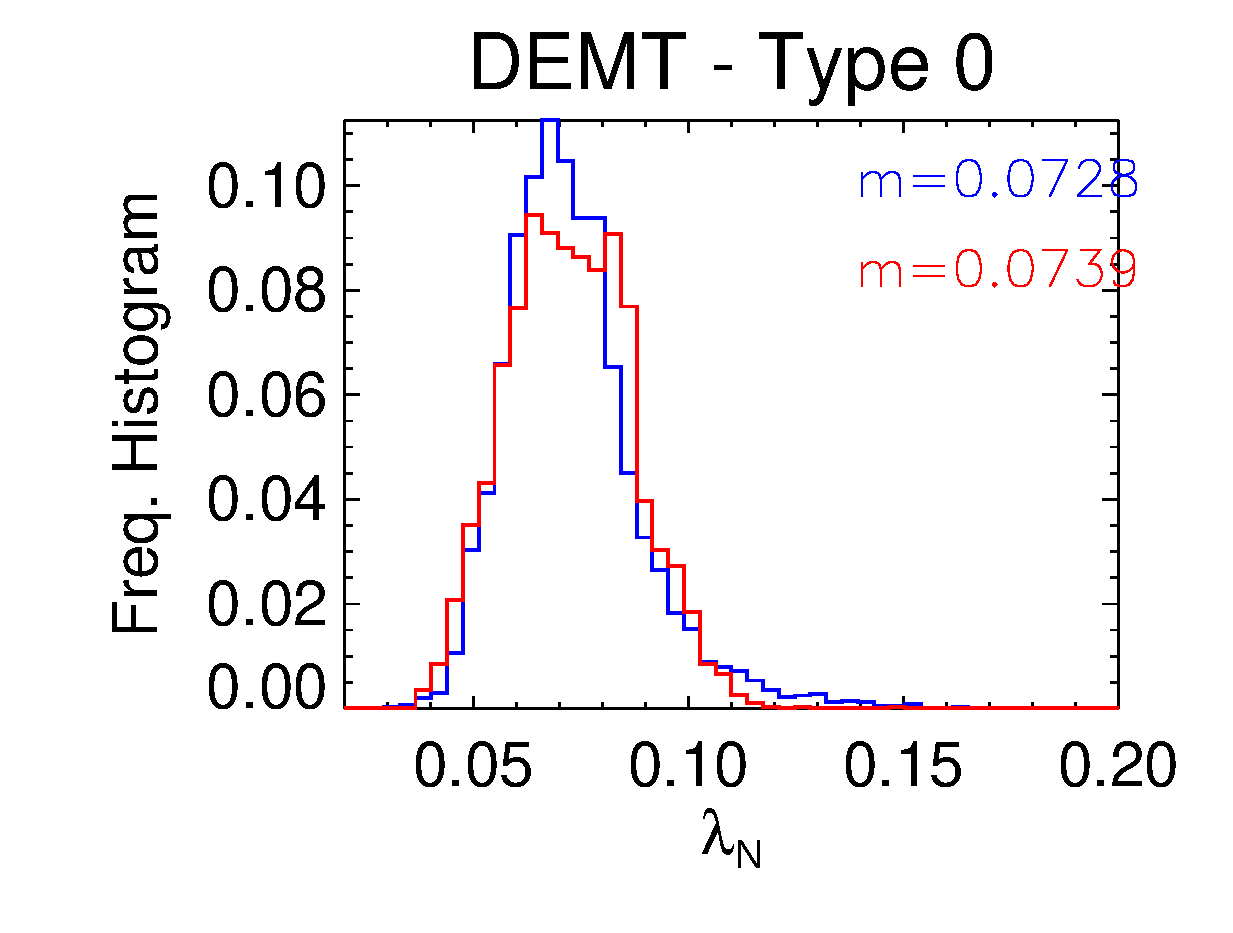
\includegraphics[width=0.31\textwidth,clip=]{figs/histo_2082_2208_fulldemt_streamer_down_lambda_n.eps}
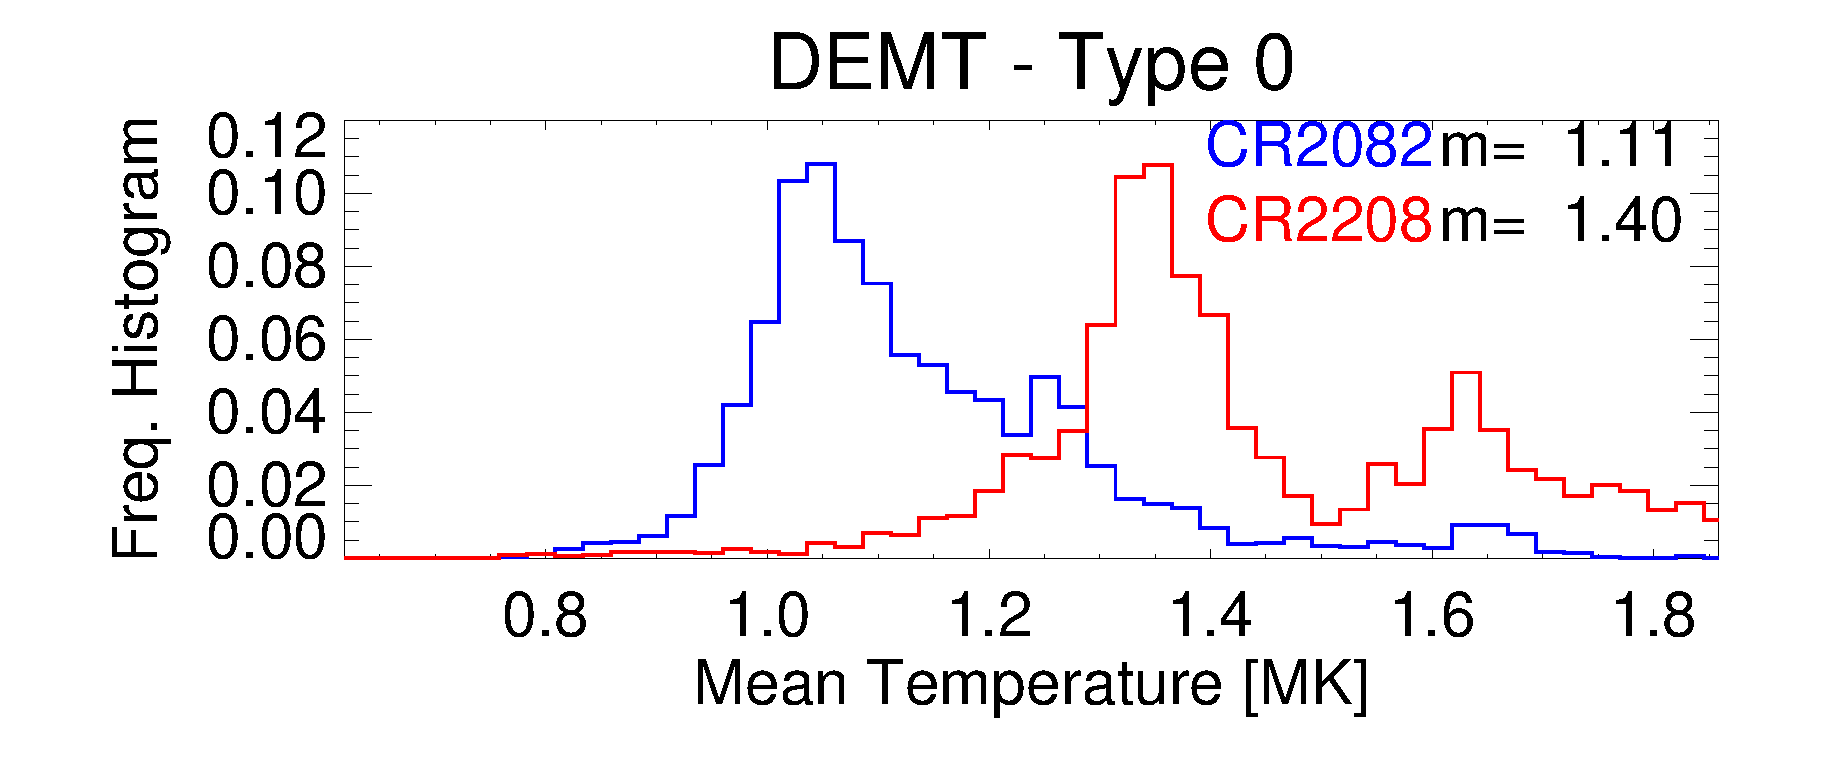
\includegraphics[width=0.31\textwidth,clip=]{figs/histo_2082_2208_fulldemt_streamer_down_Tm.eps}
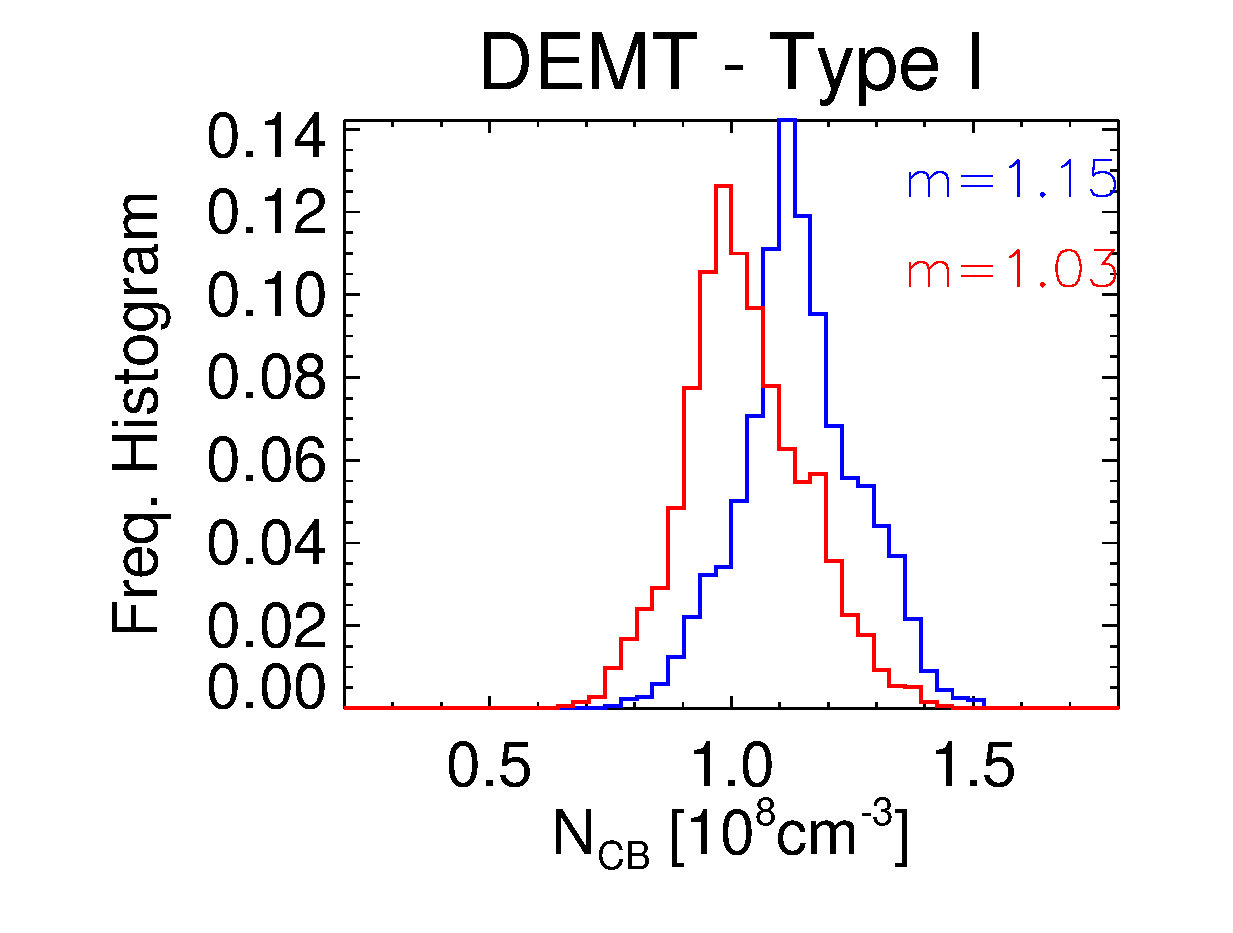
\includegraphics[width=0.31\textwidth,clip=]{figs/histo_2082_2208_fulldemt_streamer_up_ne_1055.eps}
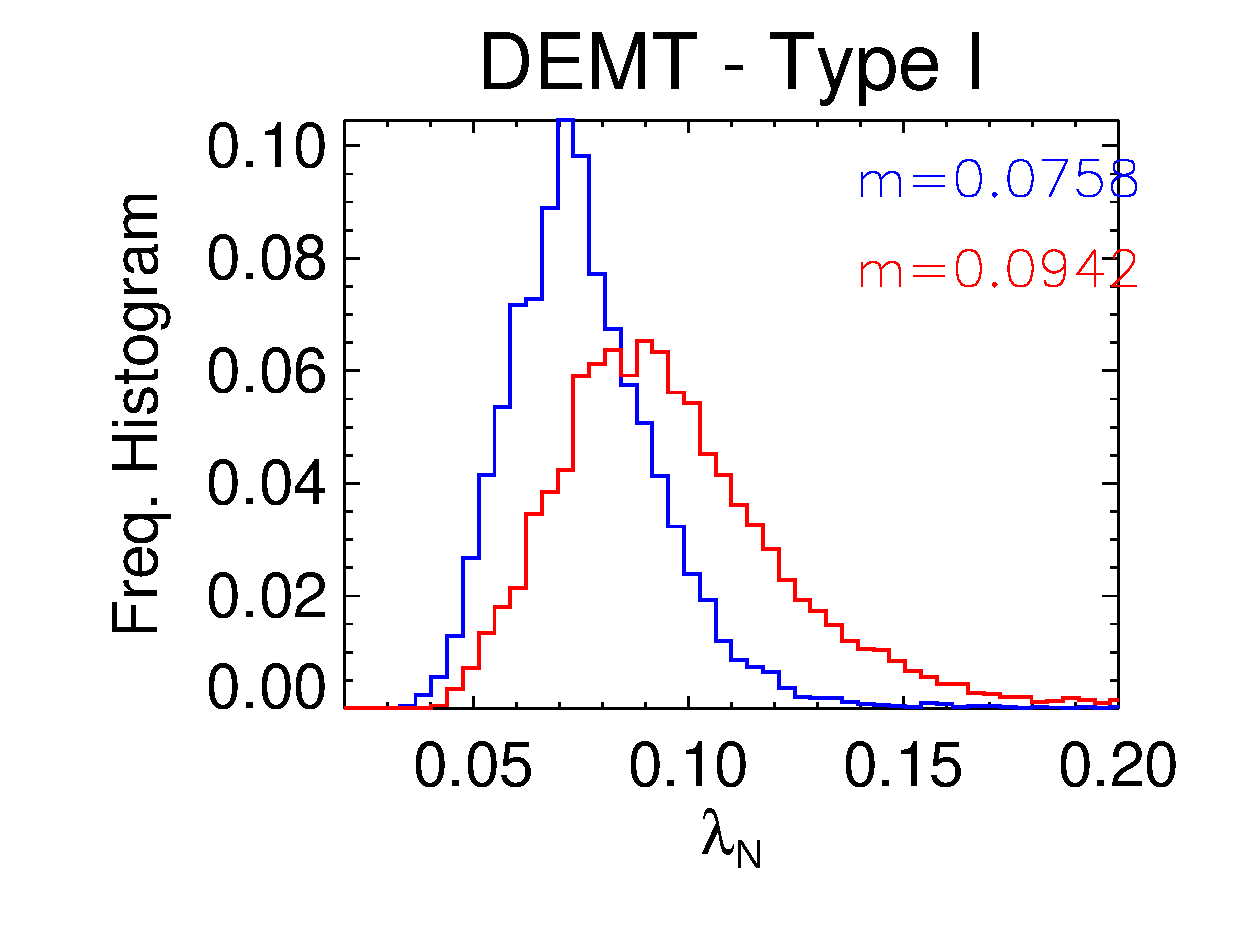
\includegraphics[width=0.31\textwidth,clip=]{figs/histo_2082_2208_fulldemt_streamer_up_lambda_n.eps}
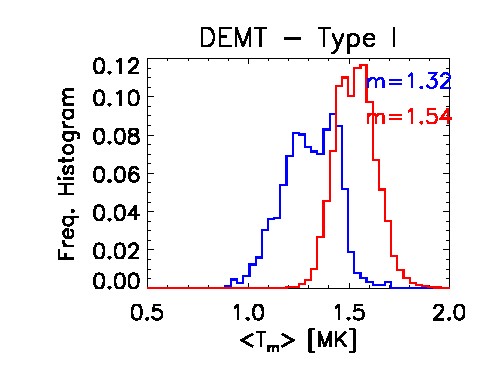
\includegraphics[width=0.31\textwidth,clip=]{figs/histo_2082_2208_fulldemt_streamer_up_Tm.eps}
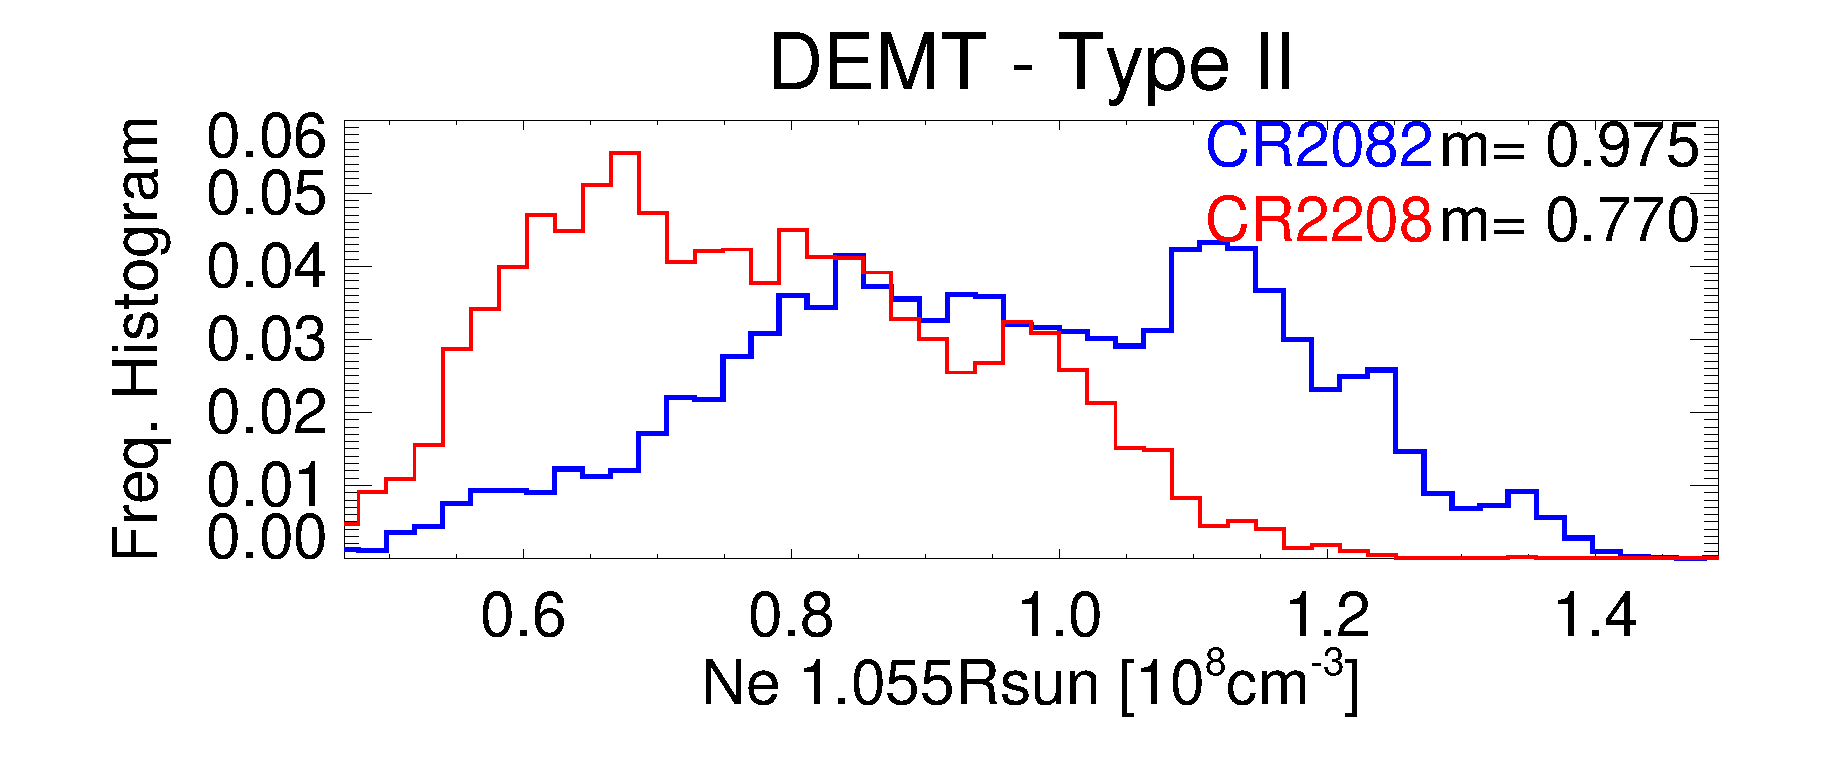
\includegraphics[width=0.31\textwidth,clip=]{figs/histo_2082_2208_fulldemt_bound_up_ne_1055.eps}
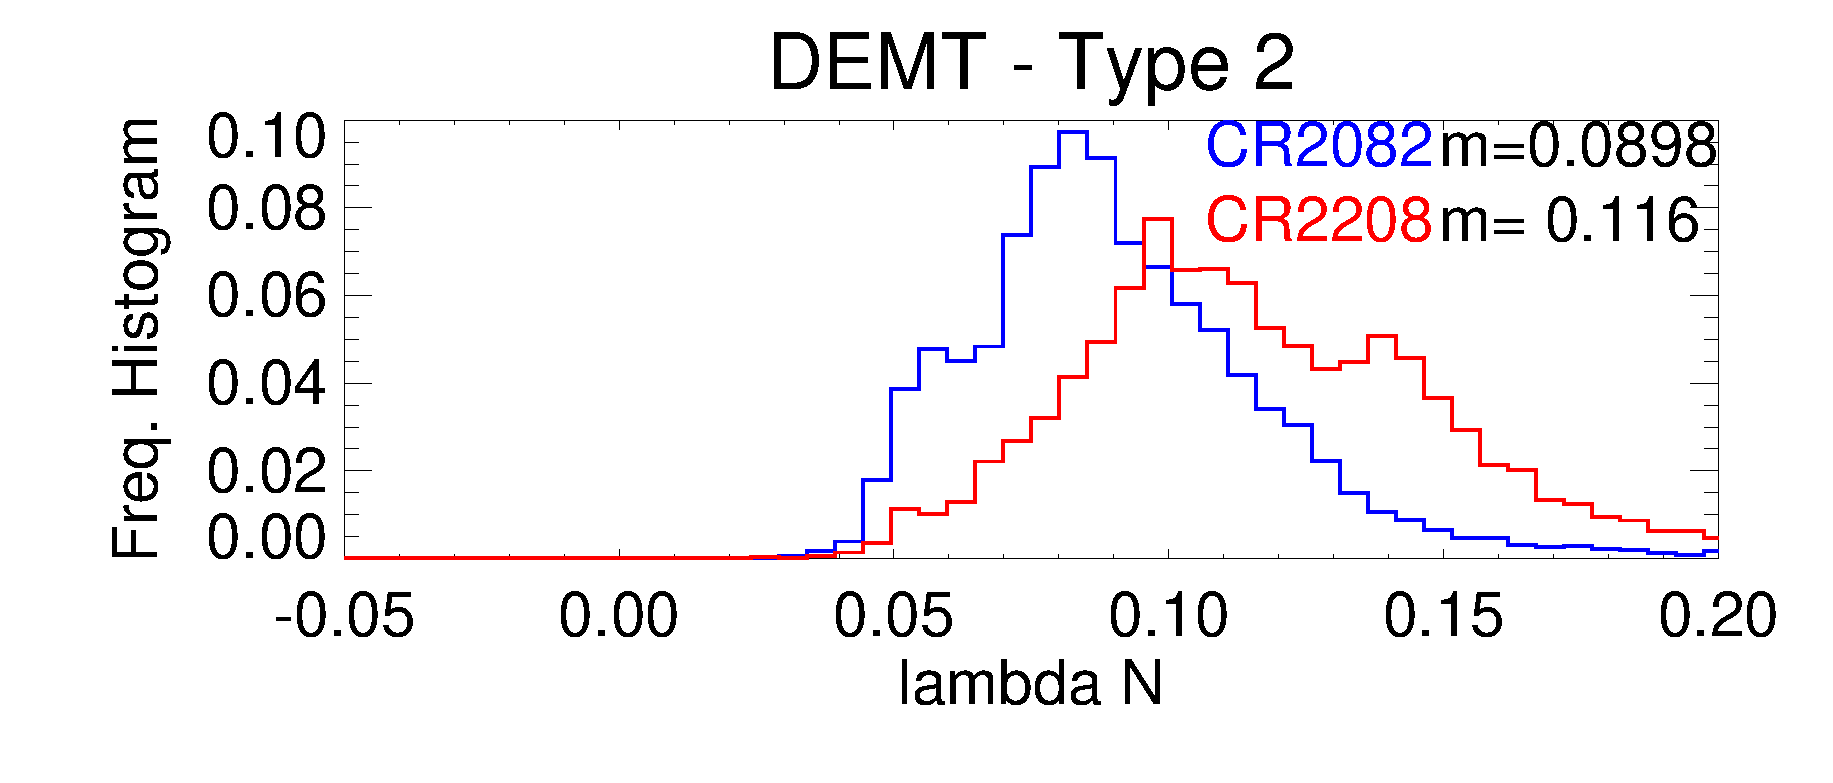
\includegraphics[width=0.31\textwidth,clip=]{figs/histo_2082_2208_fulldemt_bound_up_lambda_n.eps}
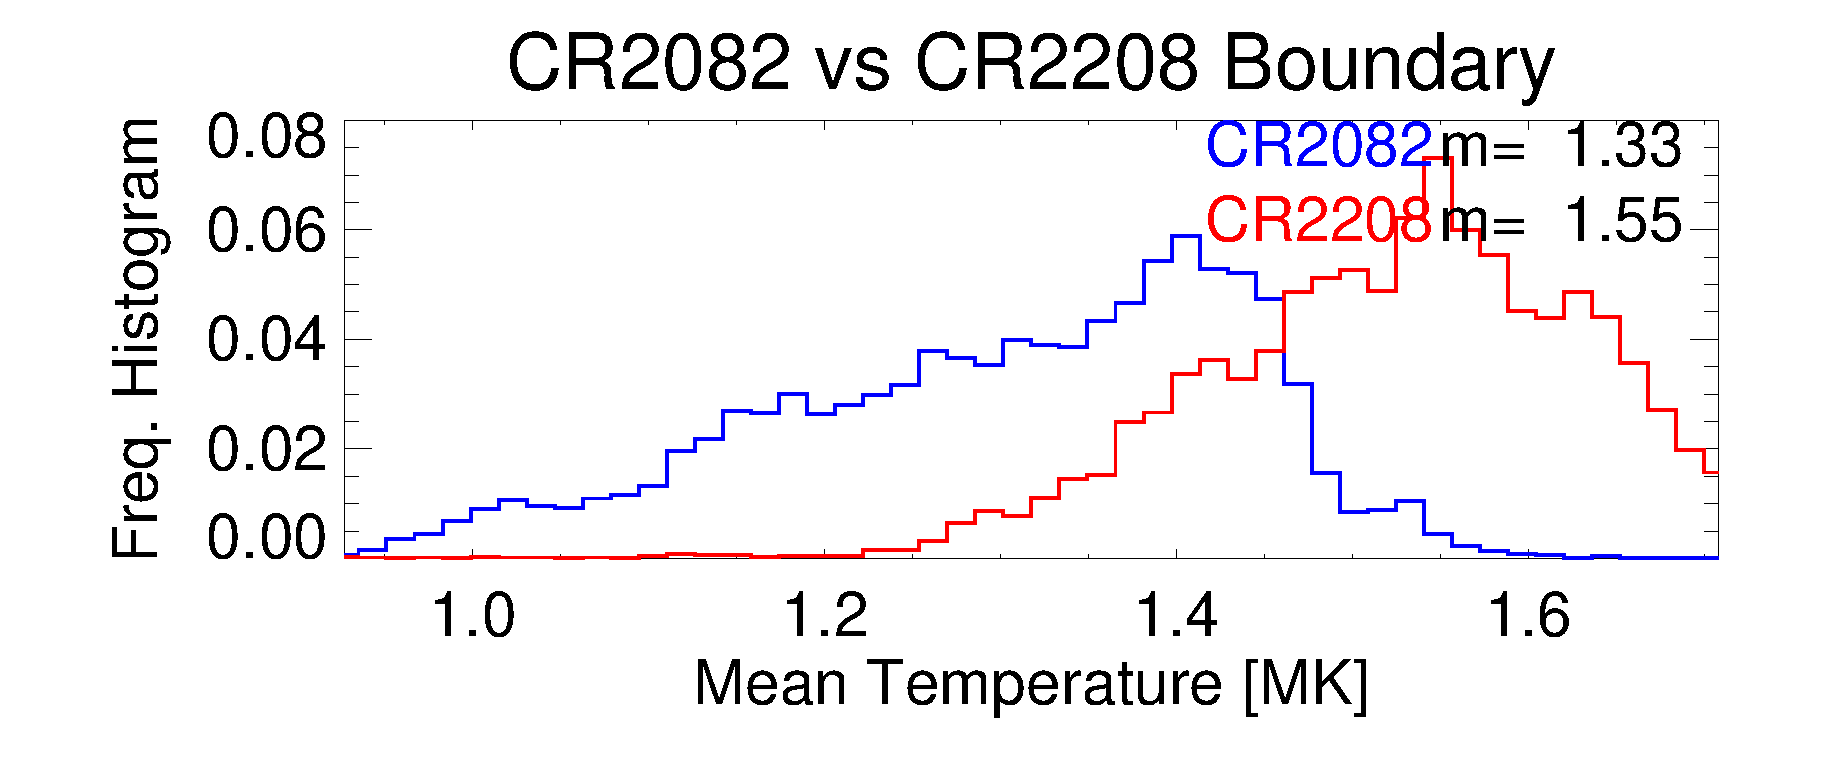
\includegraphics[width=0.31\textwidth,clip=]{figs/histo_2082_2208_fulldemt_bound_up_Tm.eps}
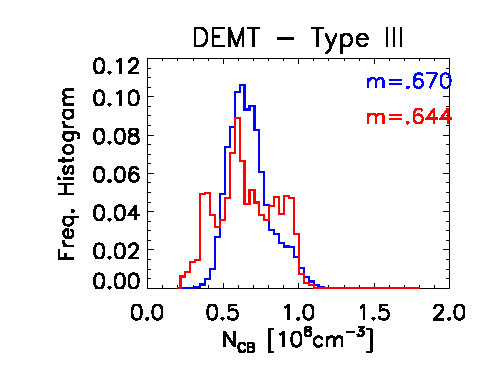
\includegraphics[width=0.31\textwidth,clip=]{figs/histo_2082_2208_fulldemt_CH_up_ne_1055.eps}
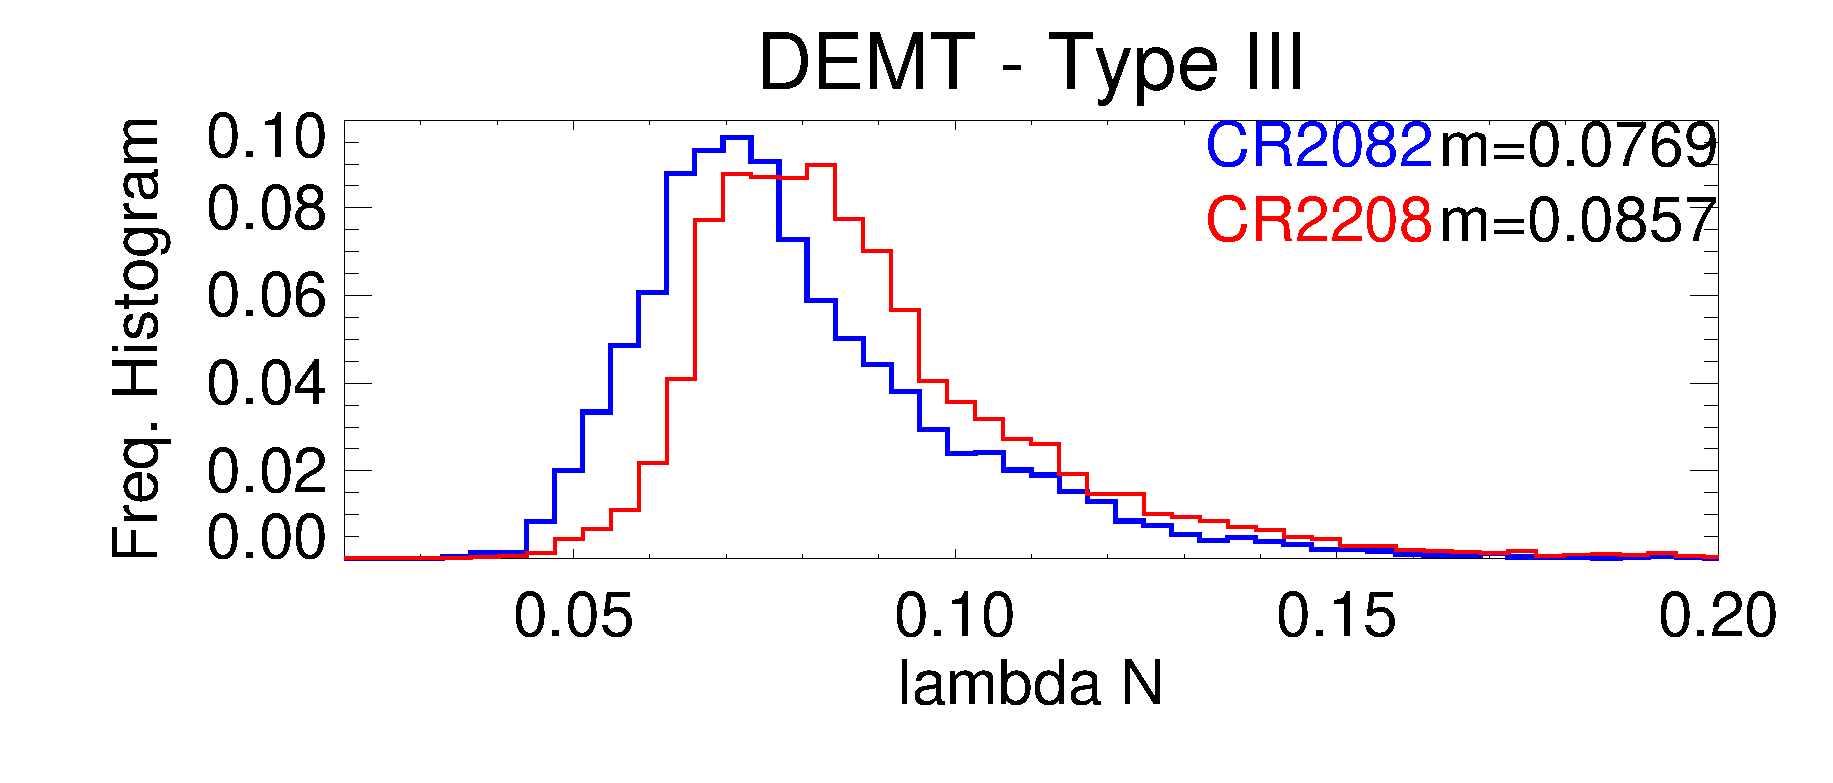
\includegraphics[width=0.31\textwidth,clip=]{figs/histo_2082_2208_fulldemt_CH_up_lambda_n.eps}
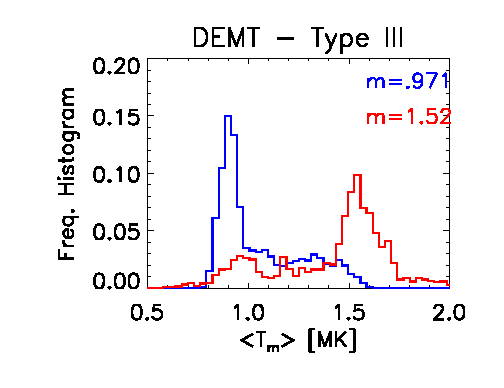
\includegraphics[width=0.31\textwidth,clip=]{figs/histo_2082_2208_fulldemt_CH_up_Tm.eps}
\caption{Comparative statistical distributions of DEMT reults. From left to right: the coronal base electron density $N_e(r=1.055\,\mrsun)$, the electron density scale height $\lN$ and the average electron mean temperature $\aTm$, along all types of legs defined in Section \ref{trace}. Results of CR2082 are shown in blue while those of CR-2208 in red. In each panel the median $m$ is indicated.}
\label{histos_fulldemt}
\end{center}
\end{figure} 


\begin{figure}[h!]
\begin{center}
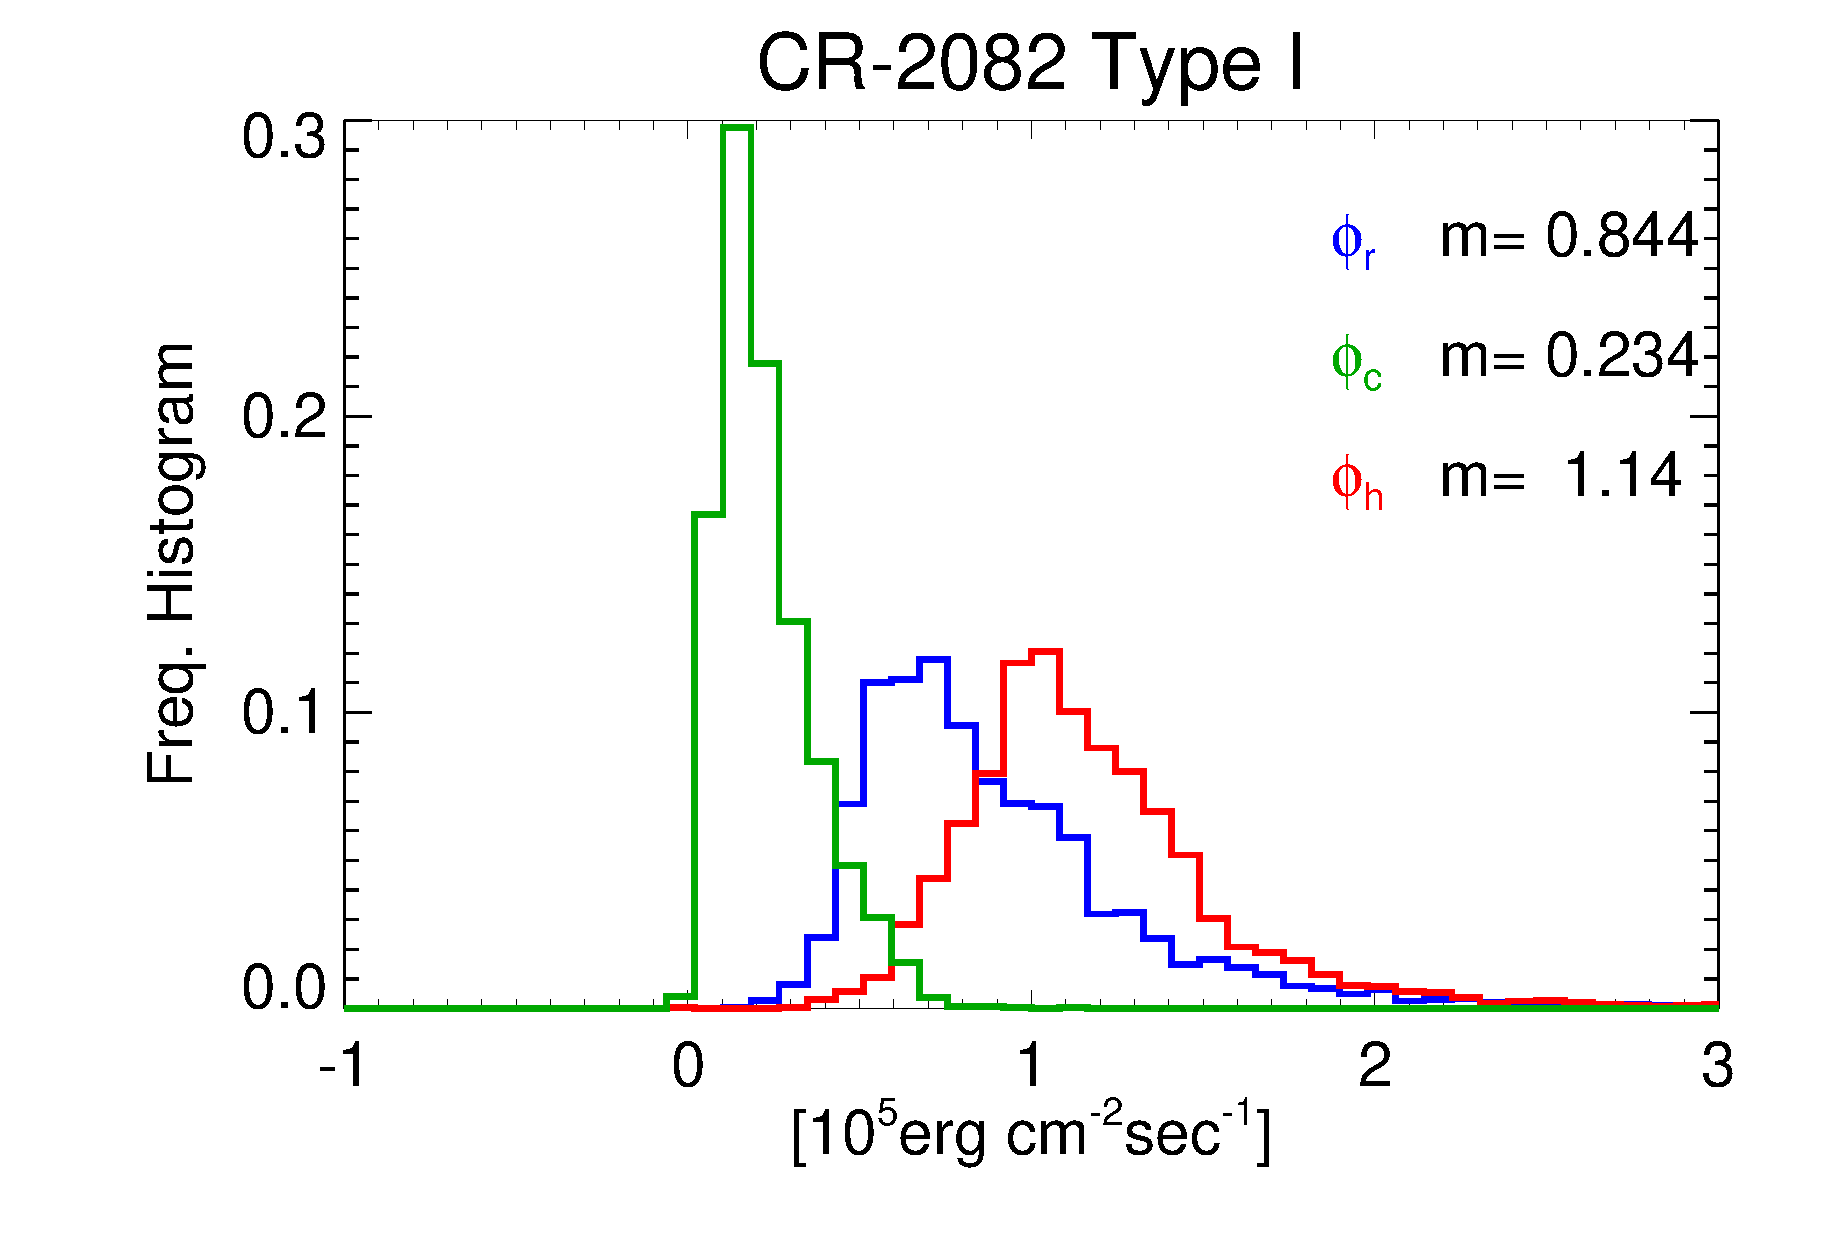
\includegraphics[width=0.495\textwidth,clip=]{figs/histocr2082_ccenergia.eps}
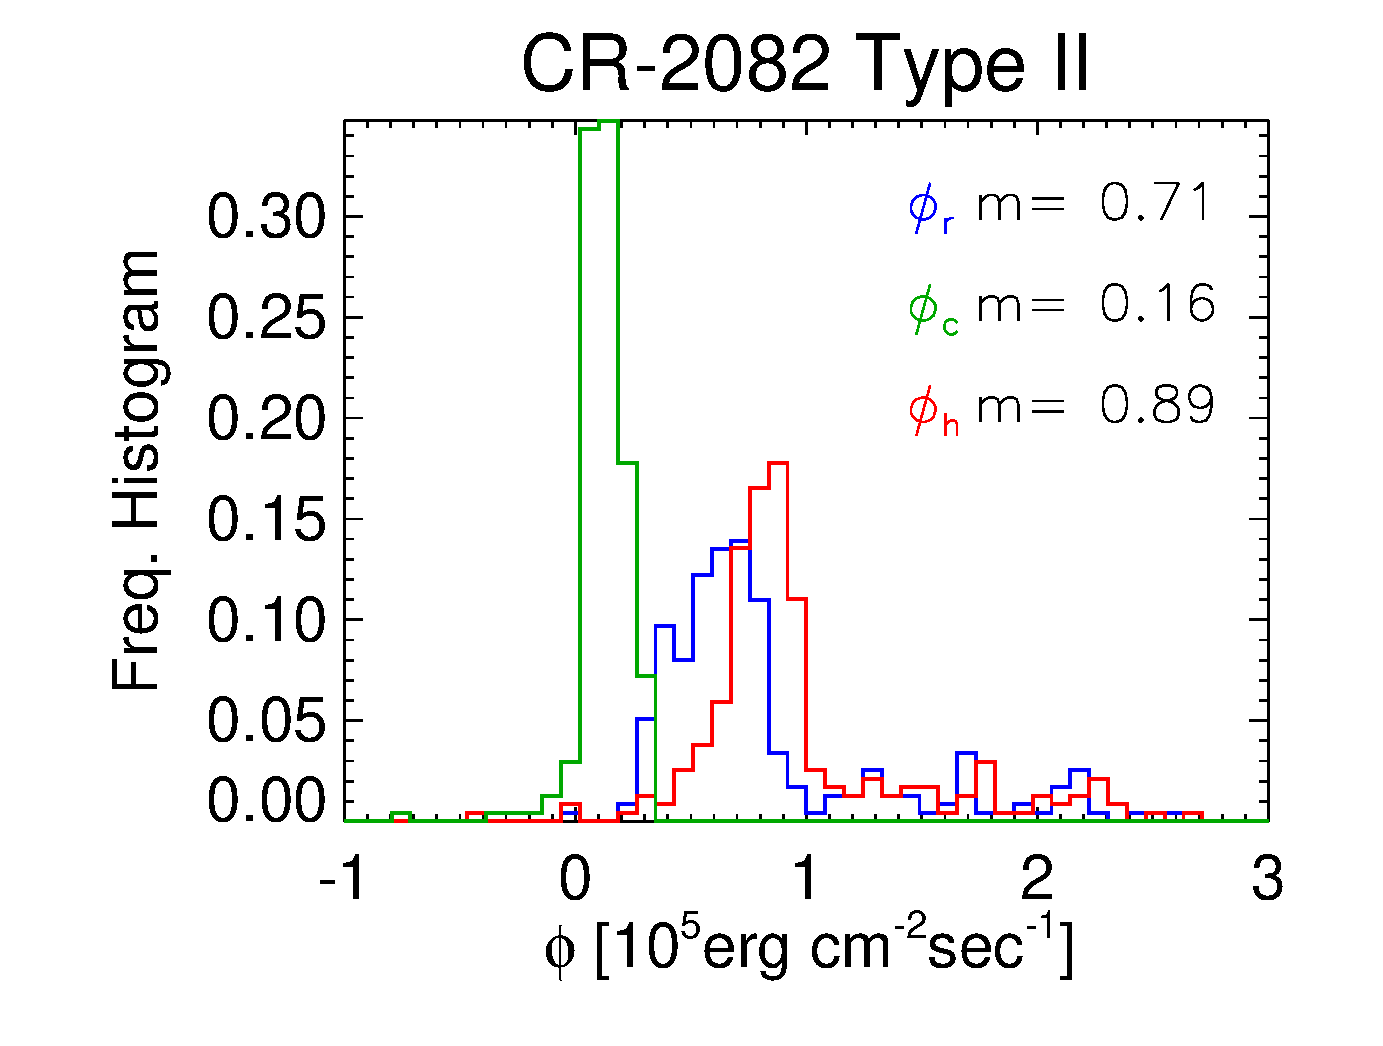
\includegraphics[width=0.495\textwidth,clip=]{figs/histocr2082_cgenergia.eps}
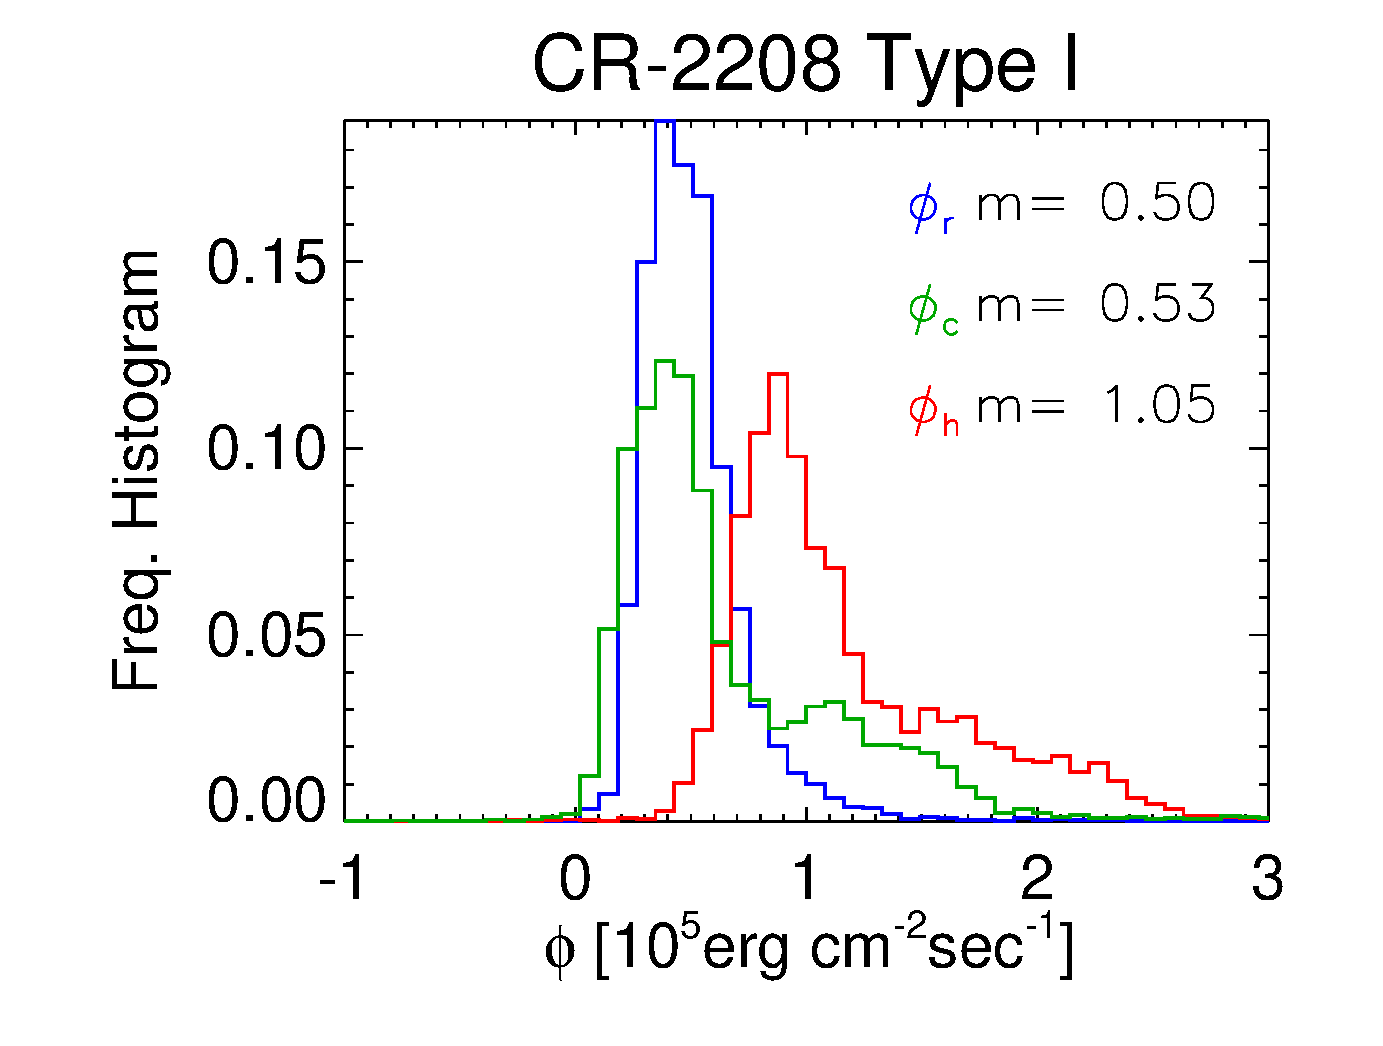
\includegraphics[width=0.495\textwidth,clip=]{figs/histocr2208_ccenergia.eps}
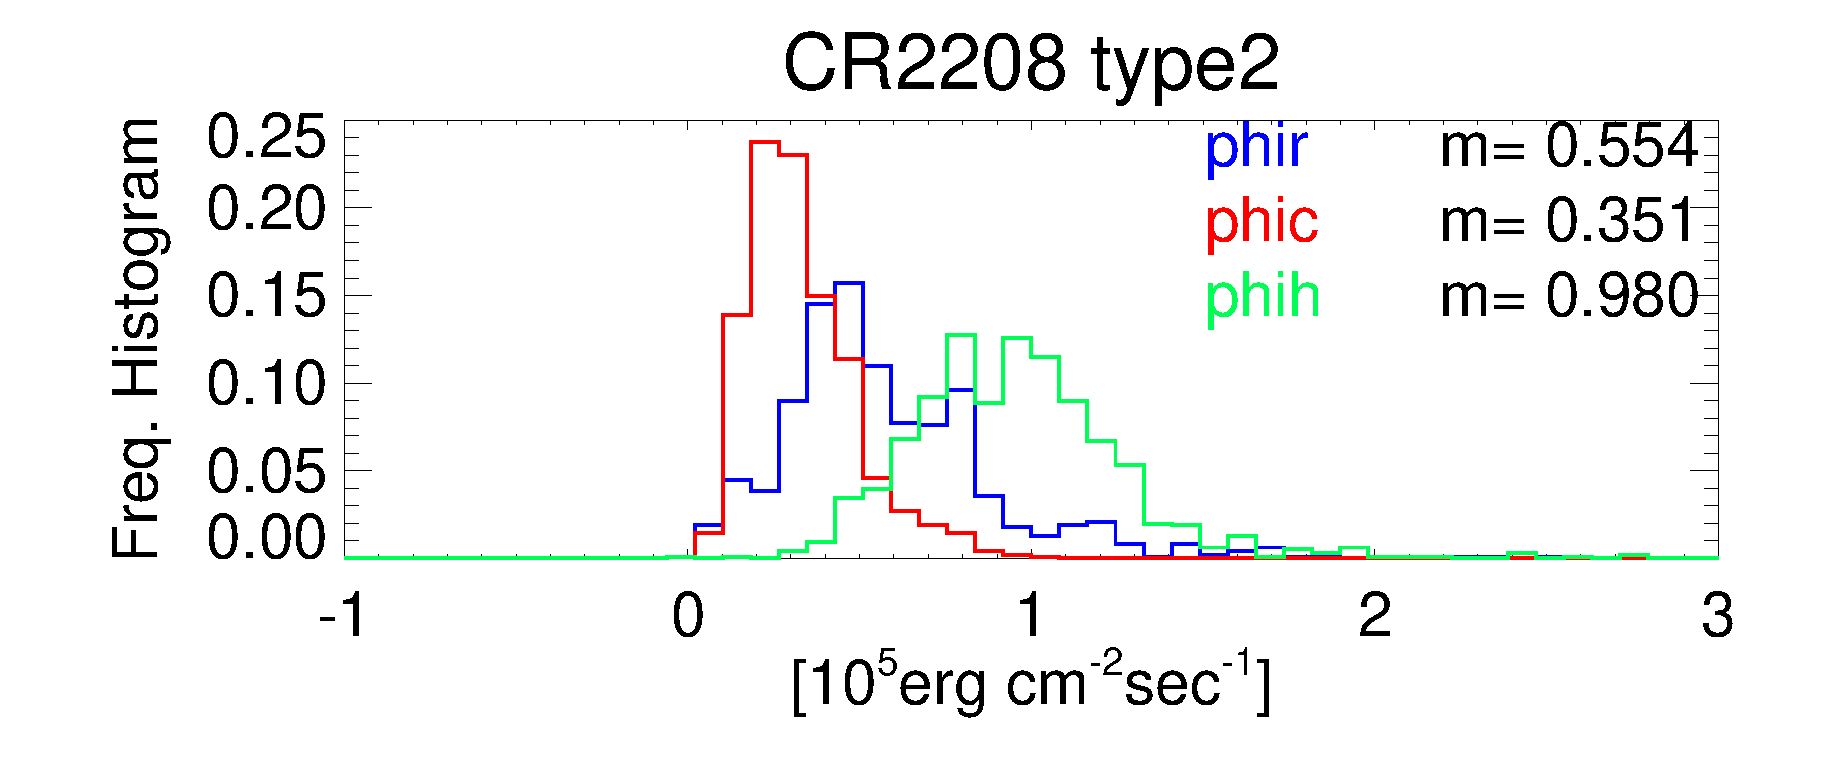
\includegraphics[width=0.495\textwidth,clip=]{figs/histocr2208_cgenergia.eps}
\caption{Statistical results of the loop integrated energy flux quantities $\phi_r,\phi_c,$ and $\phi_h$ for CR-2082 (top) and CR-2208 (bottom). Left/right panels correspond to the type 0-1 and type 2 respectively \textcolor{red}{el tipo 2 tmb tiene down! Aca hay que tomar una desicion para no marear al lector! Pero lo dejo asi internamente para compararlo con figura 5 y 6 del paper de Mac Cormack. Fede sugiere 6 graf, uno para cada tipo de linea (0, 1, 2).}}
\label{gradt_demt}
\end{center}
\end{figure} 




\subsection{Tomography and Models}\label{awsom_res} 

\textcolor{red}{Se presentan los resultados de Ne y Te del modelo AWSoM}

\begin{figure}[h!]
\begin{center}
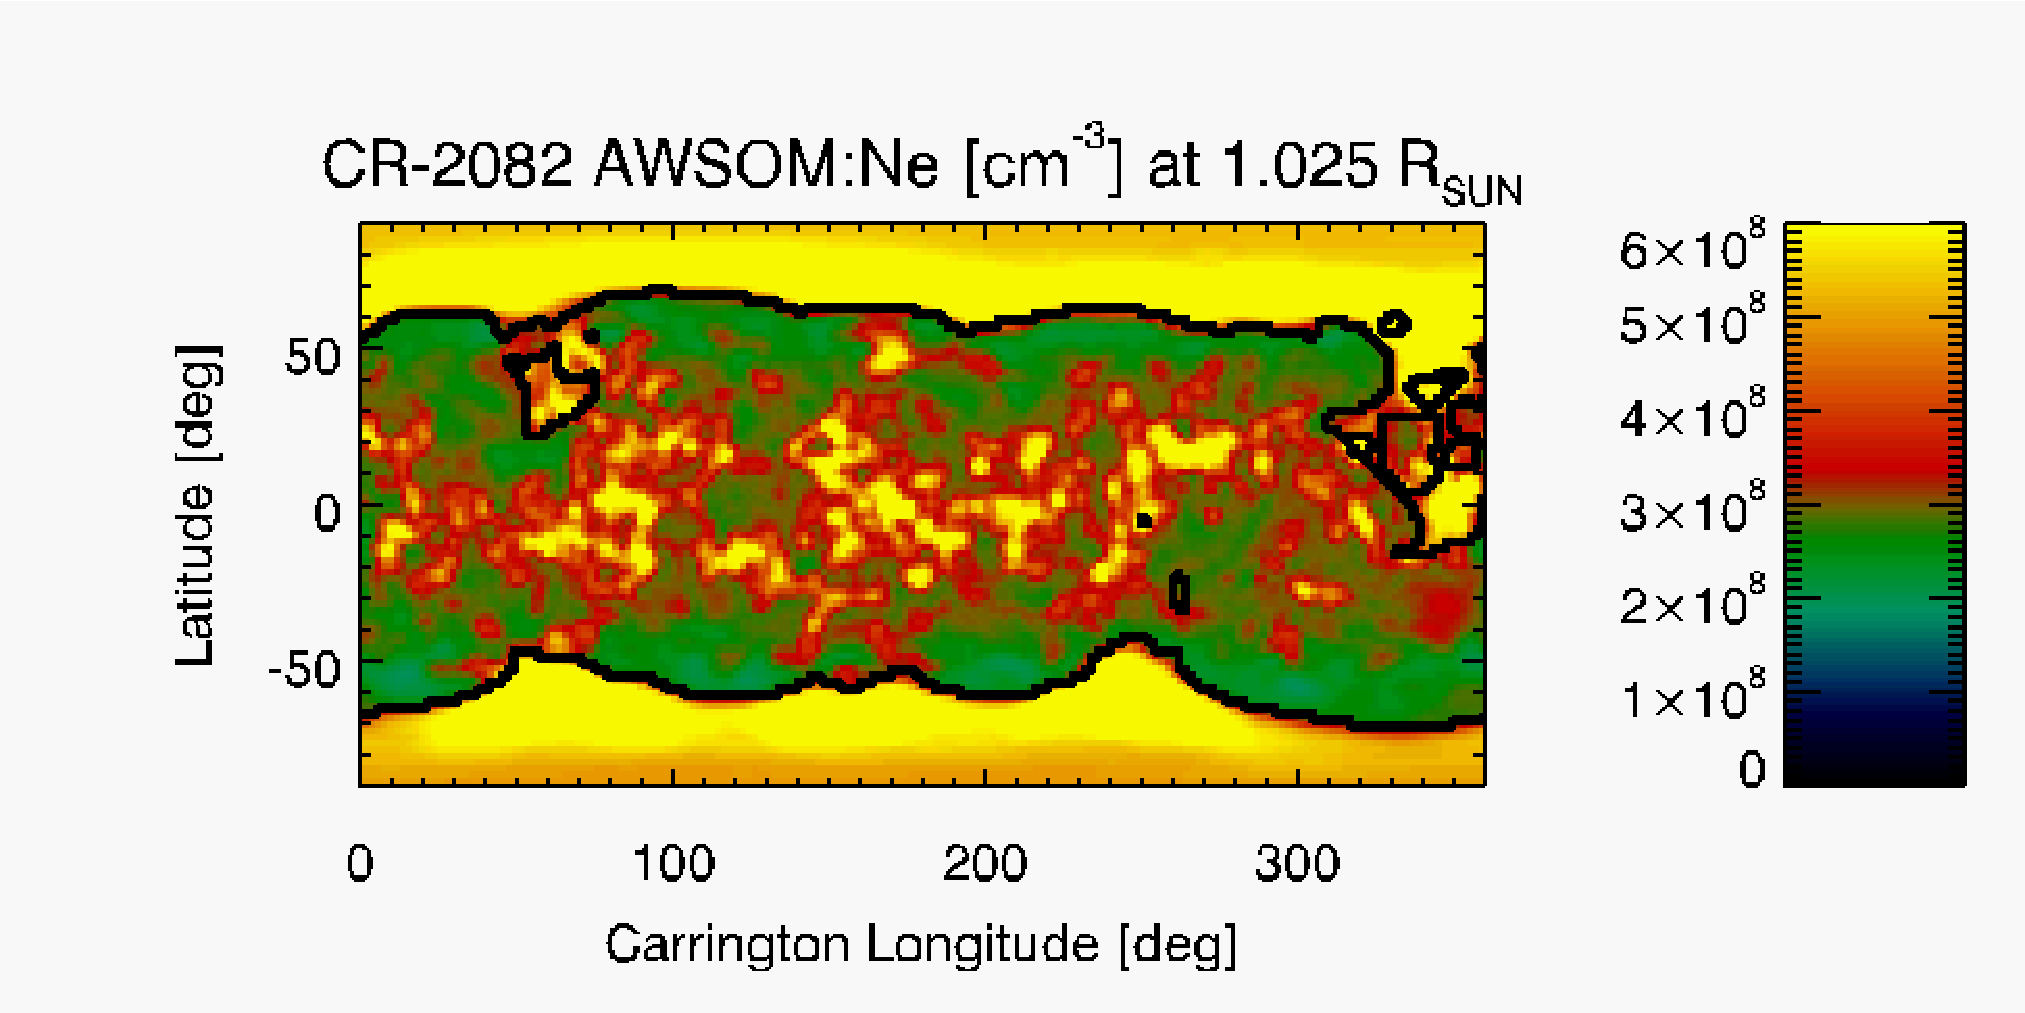
\includegraphics[width=0.495\textwidth]{figs/map_Ne_awsom_2082_185_short_1025_Rsun.pdf}
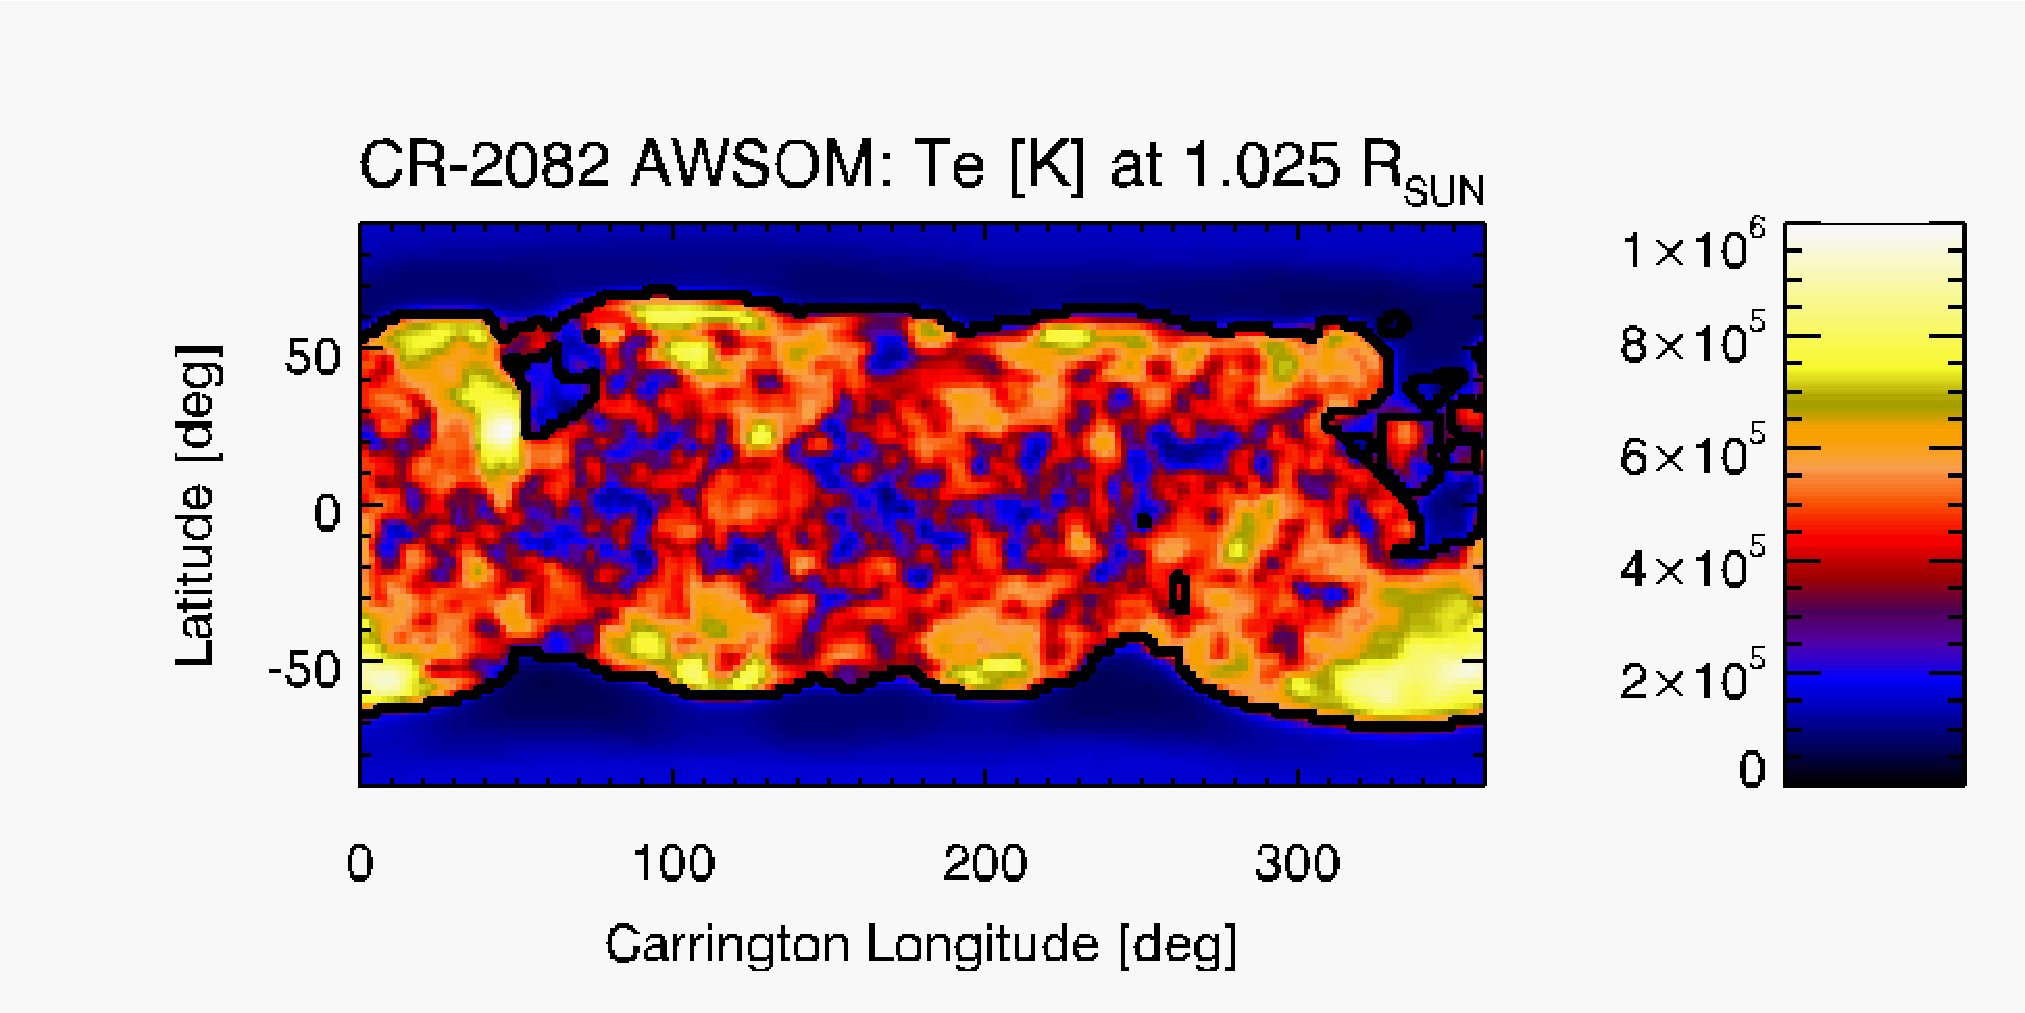
\includegraphics[width=0.495\textwidth]{figs/map_Te_awsom_2082_185_short_1025_Rsun.pdf}
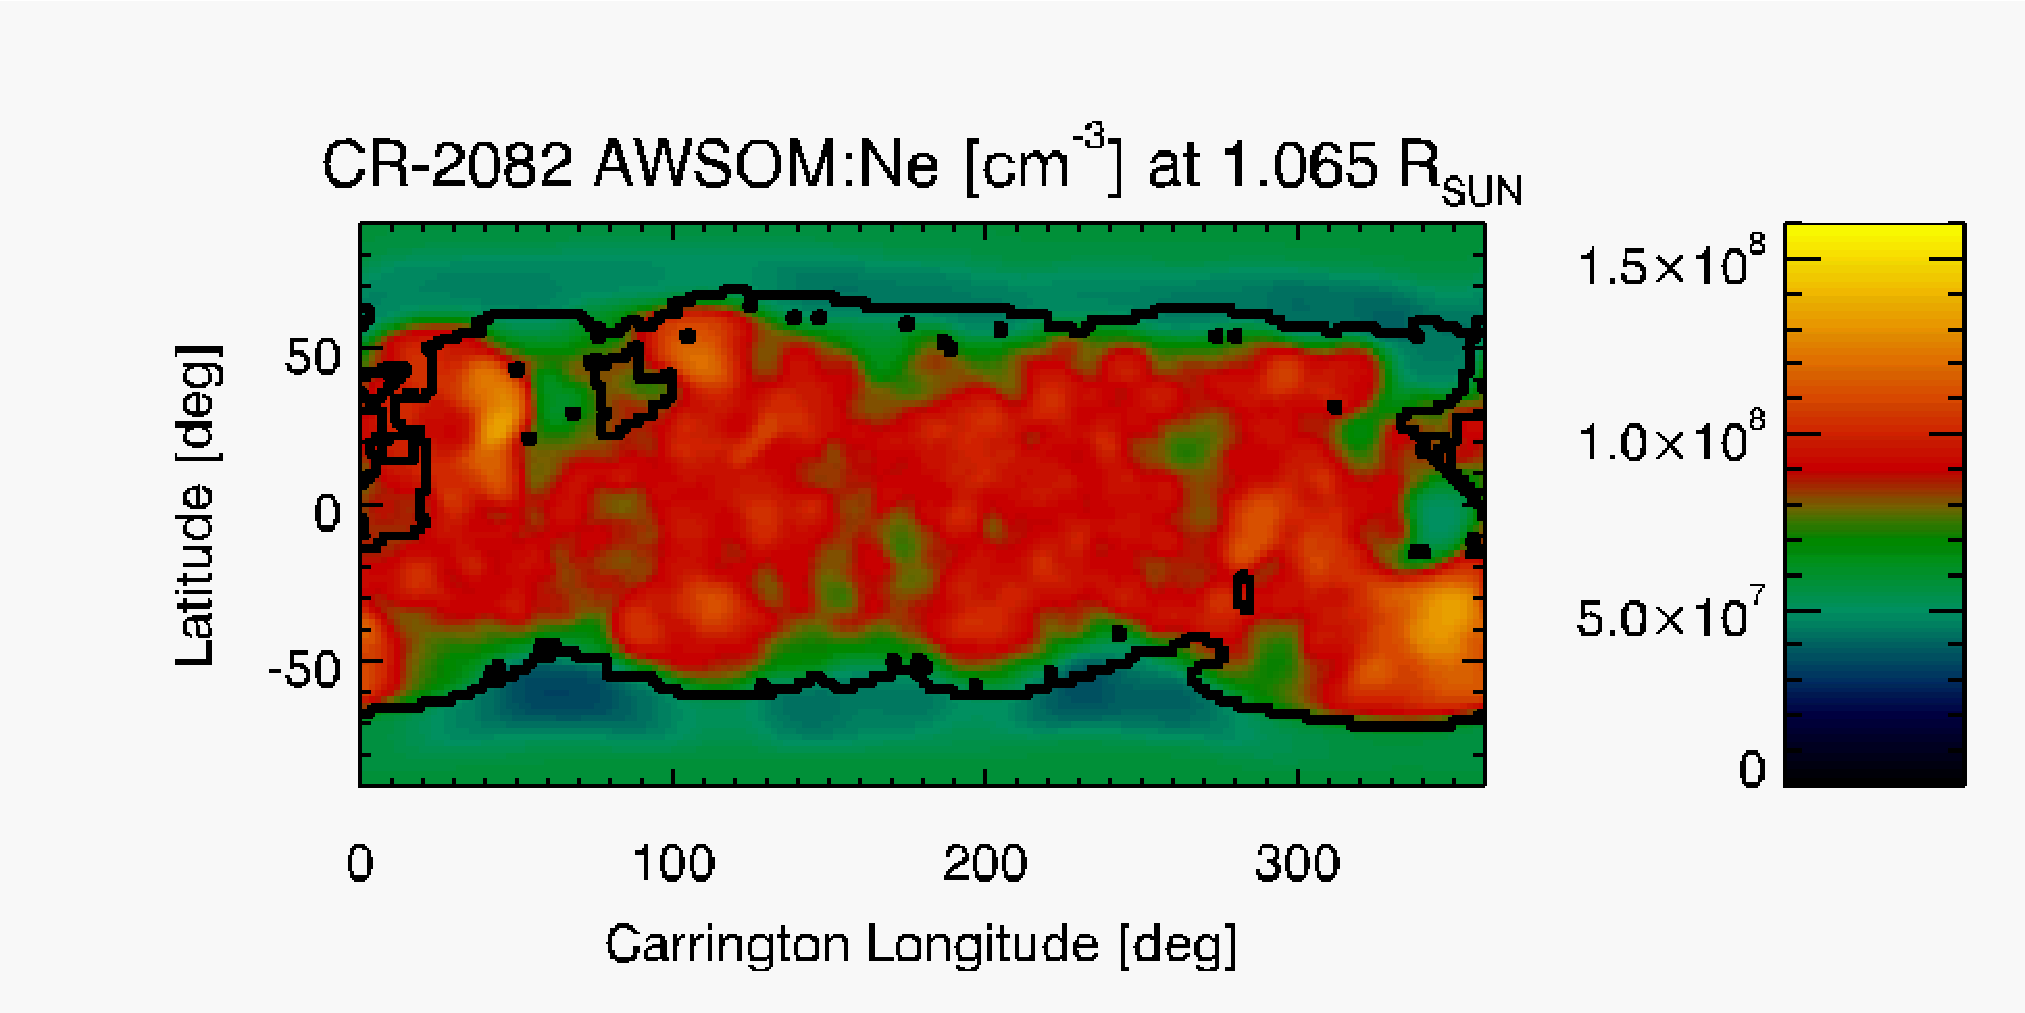
\includegraphics[width=0.495\textwidth]{figs/map_Ne_awsom_2082_185_short_1065_Rsun.pdf}
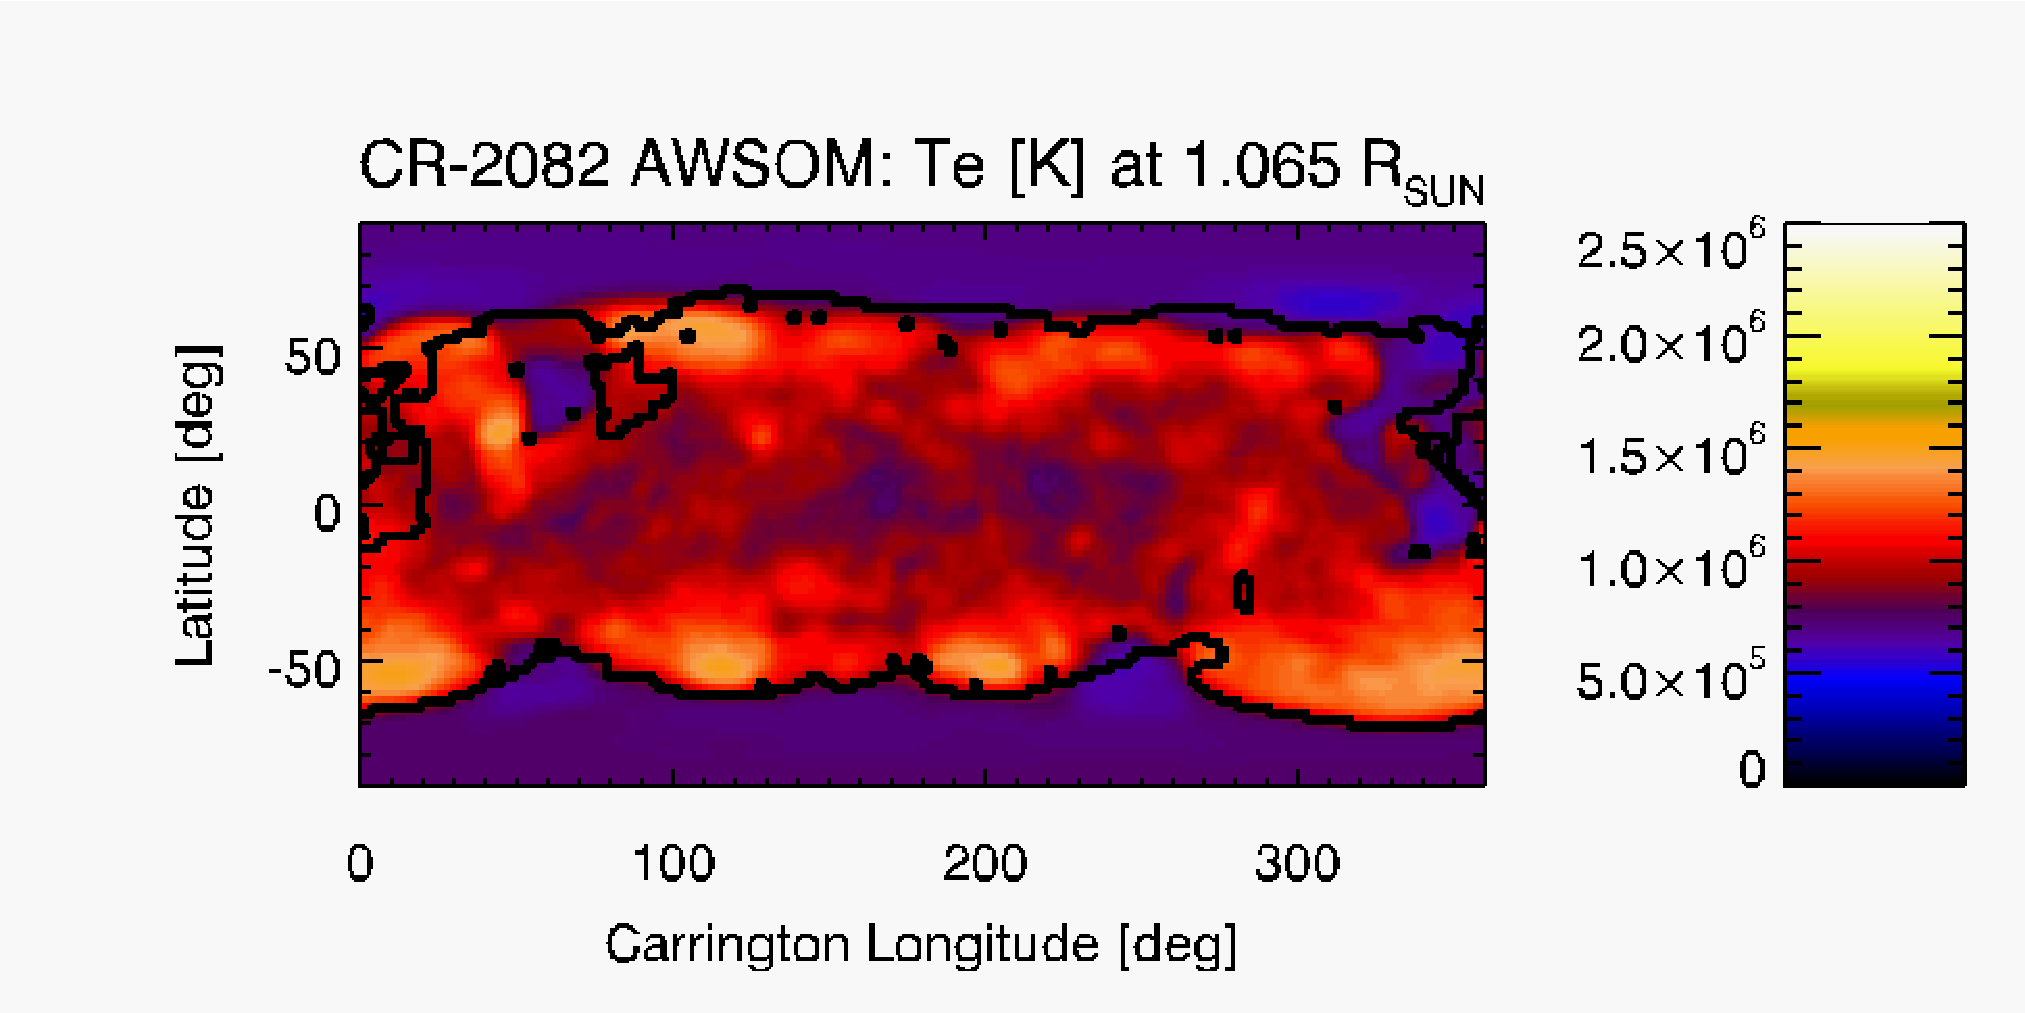
\includegraphics[width=0.495\textwidth]{figs/map_Te_awsom_2082_185_short_1065_Rsun.pdf}
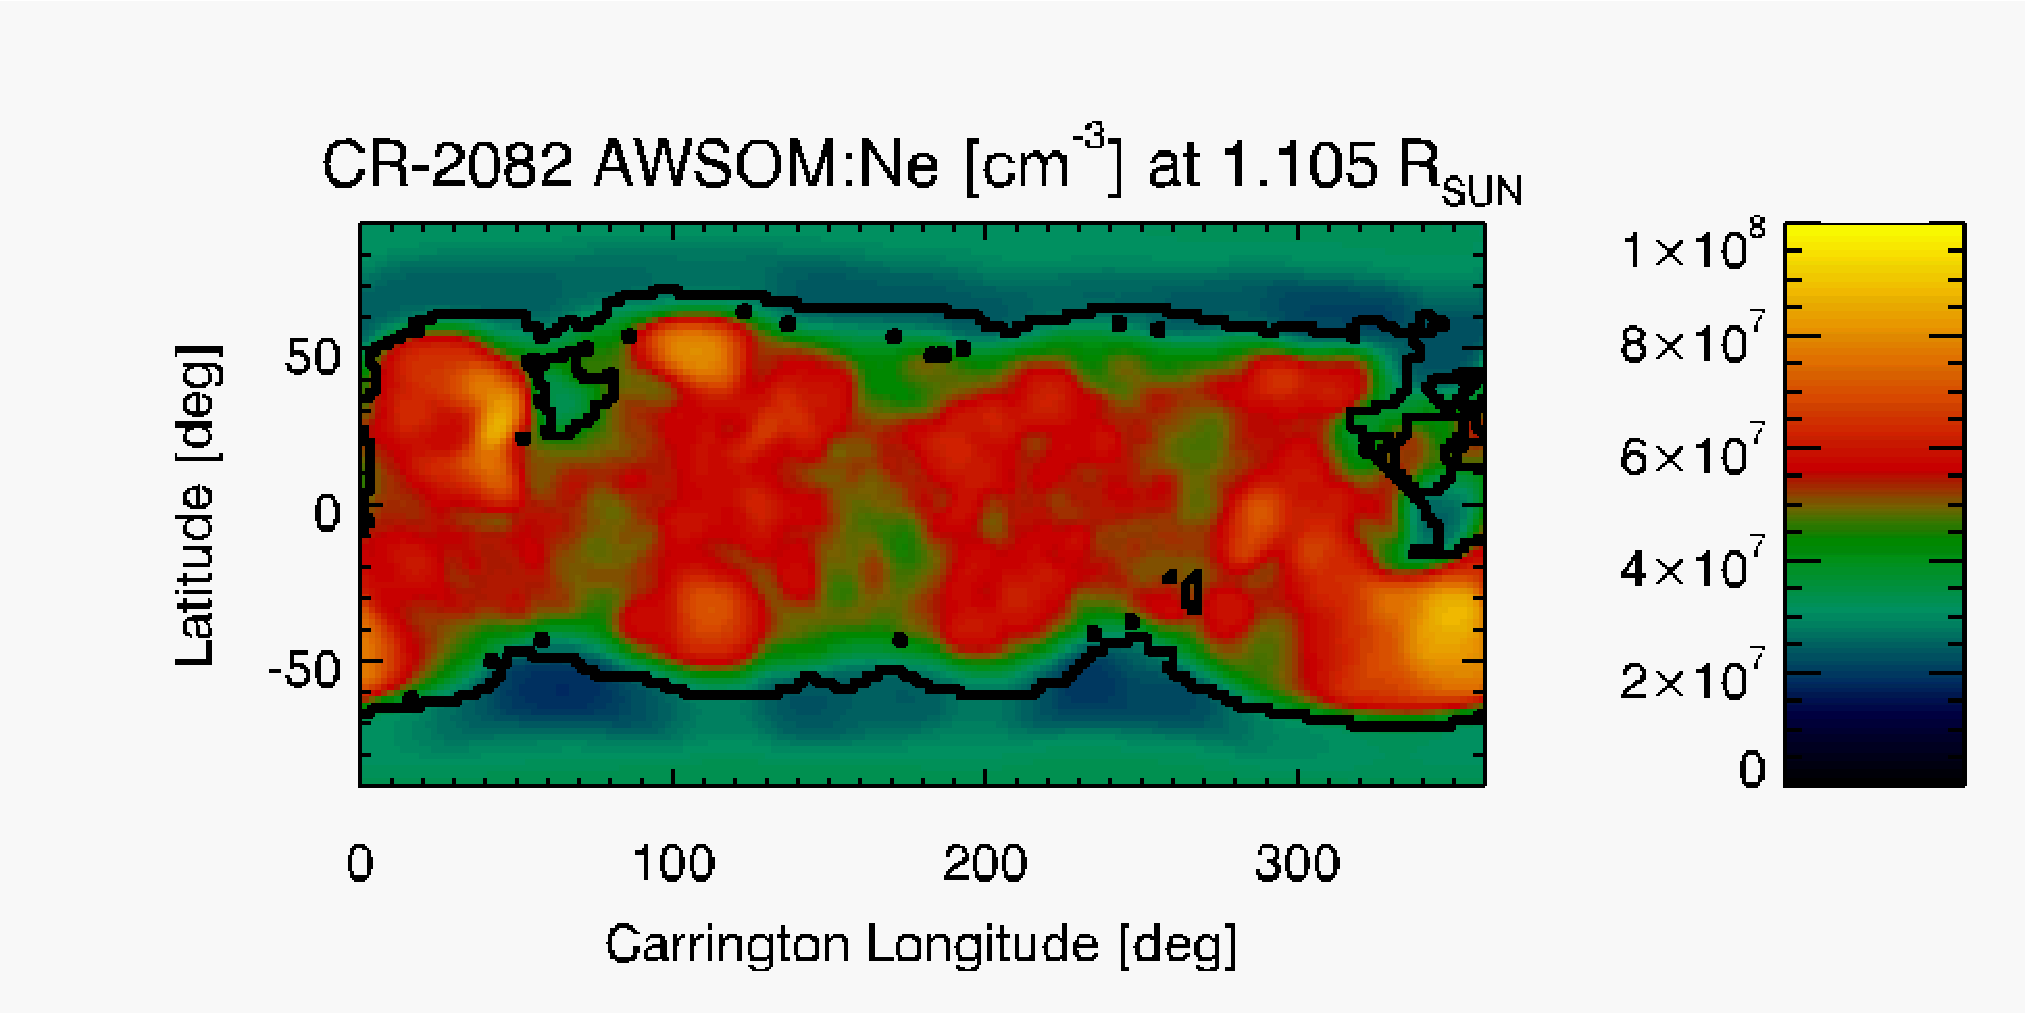
\includegraphics[width=0.495\textwidth]{figs/map_Ne_awsom_2082_185_short_1105_Rsun.pdf}
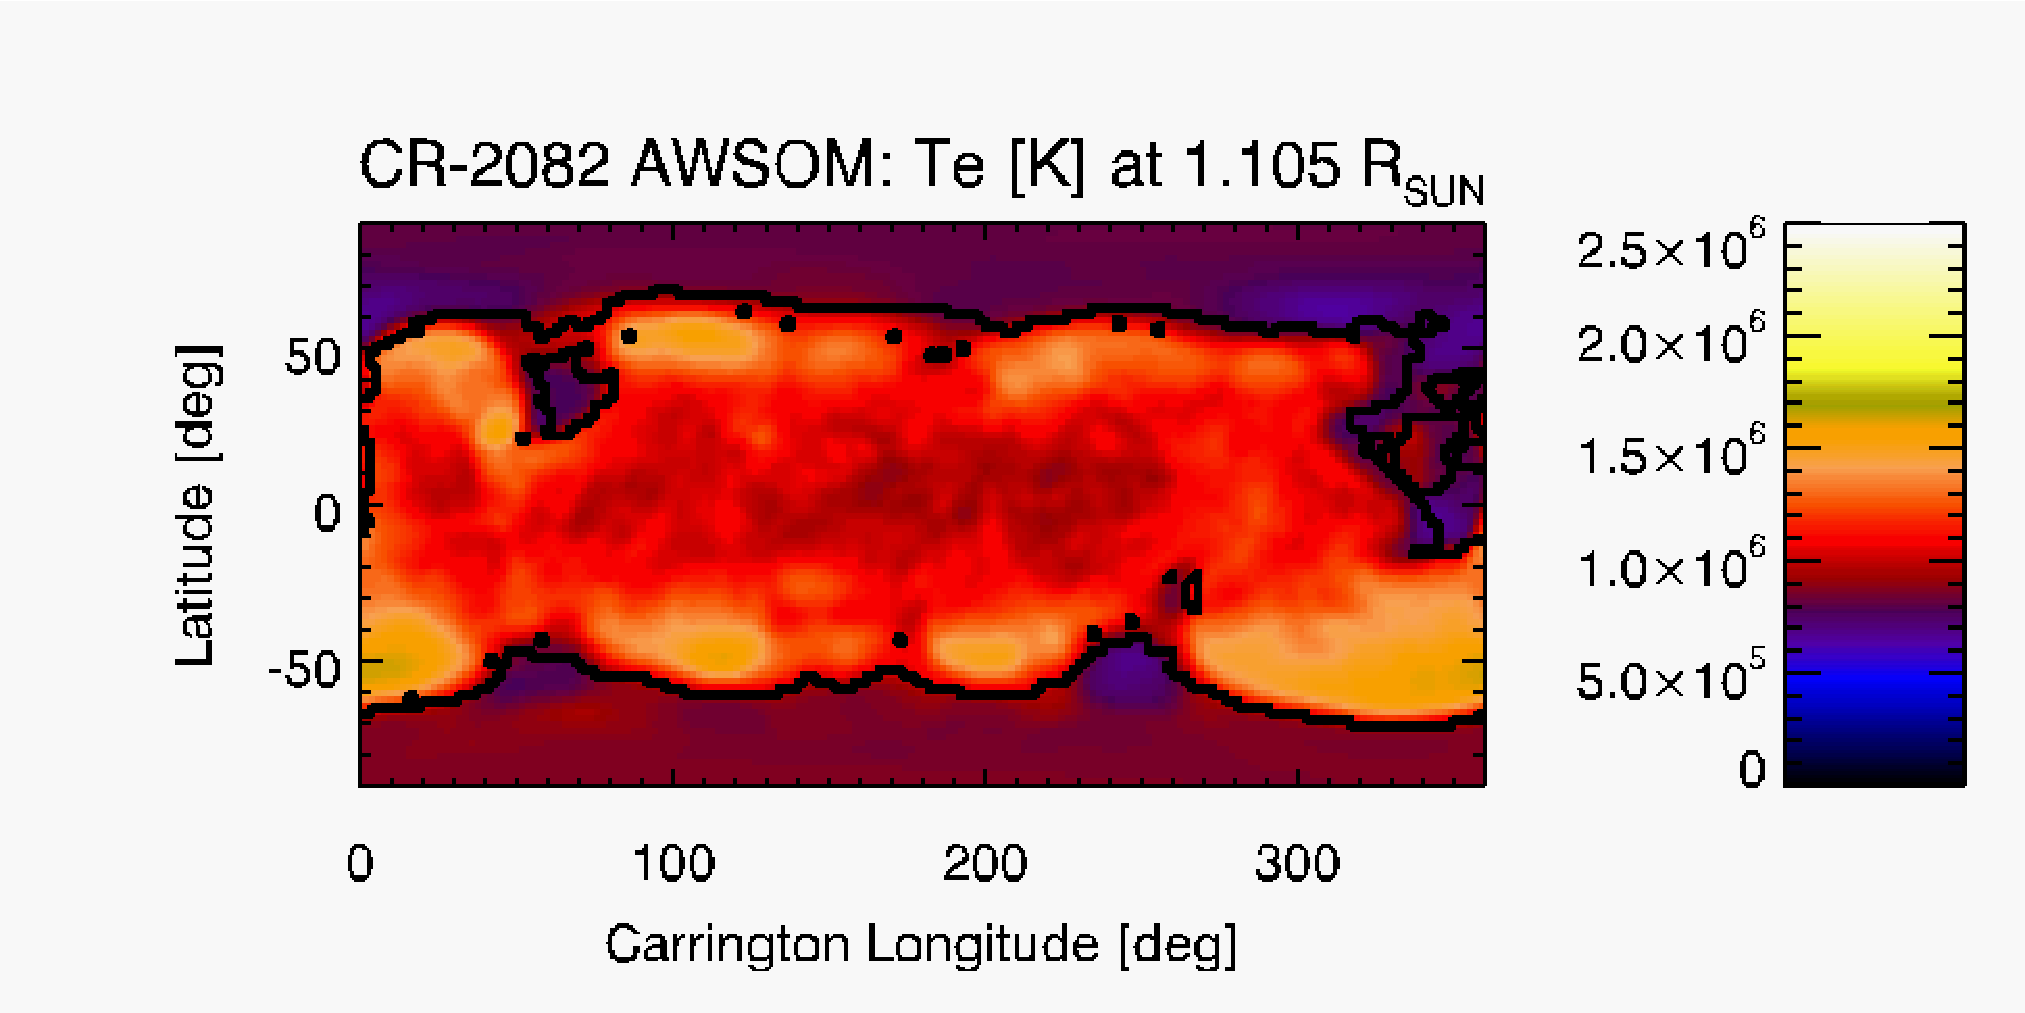
\includegraphics[width=0.495\textwidth]{figs/map_Te_awsom_2082_185_short_1105_Rsun.pdf}
\caption{Carrington maps of density (left panels) and temperature (right panels)) obtained with AWSoM model for the three heights shown in Figure \ref{carmaps_awsom_2082}.}
\label{carmaps_awsom_2082}
\end{center}
\end{figure}

\begin{figure}[h!]
\begin{center}
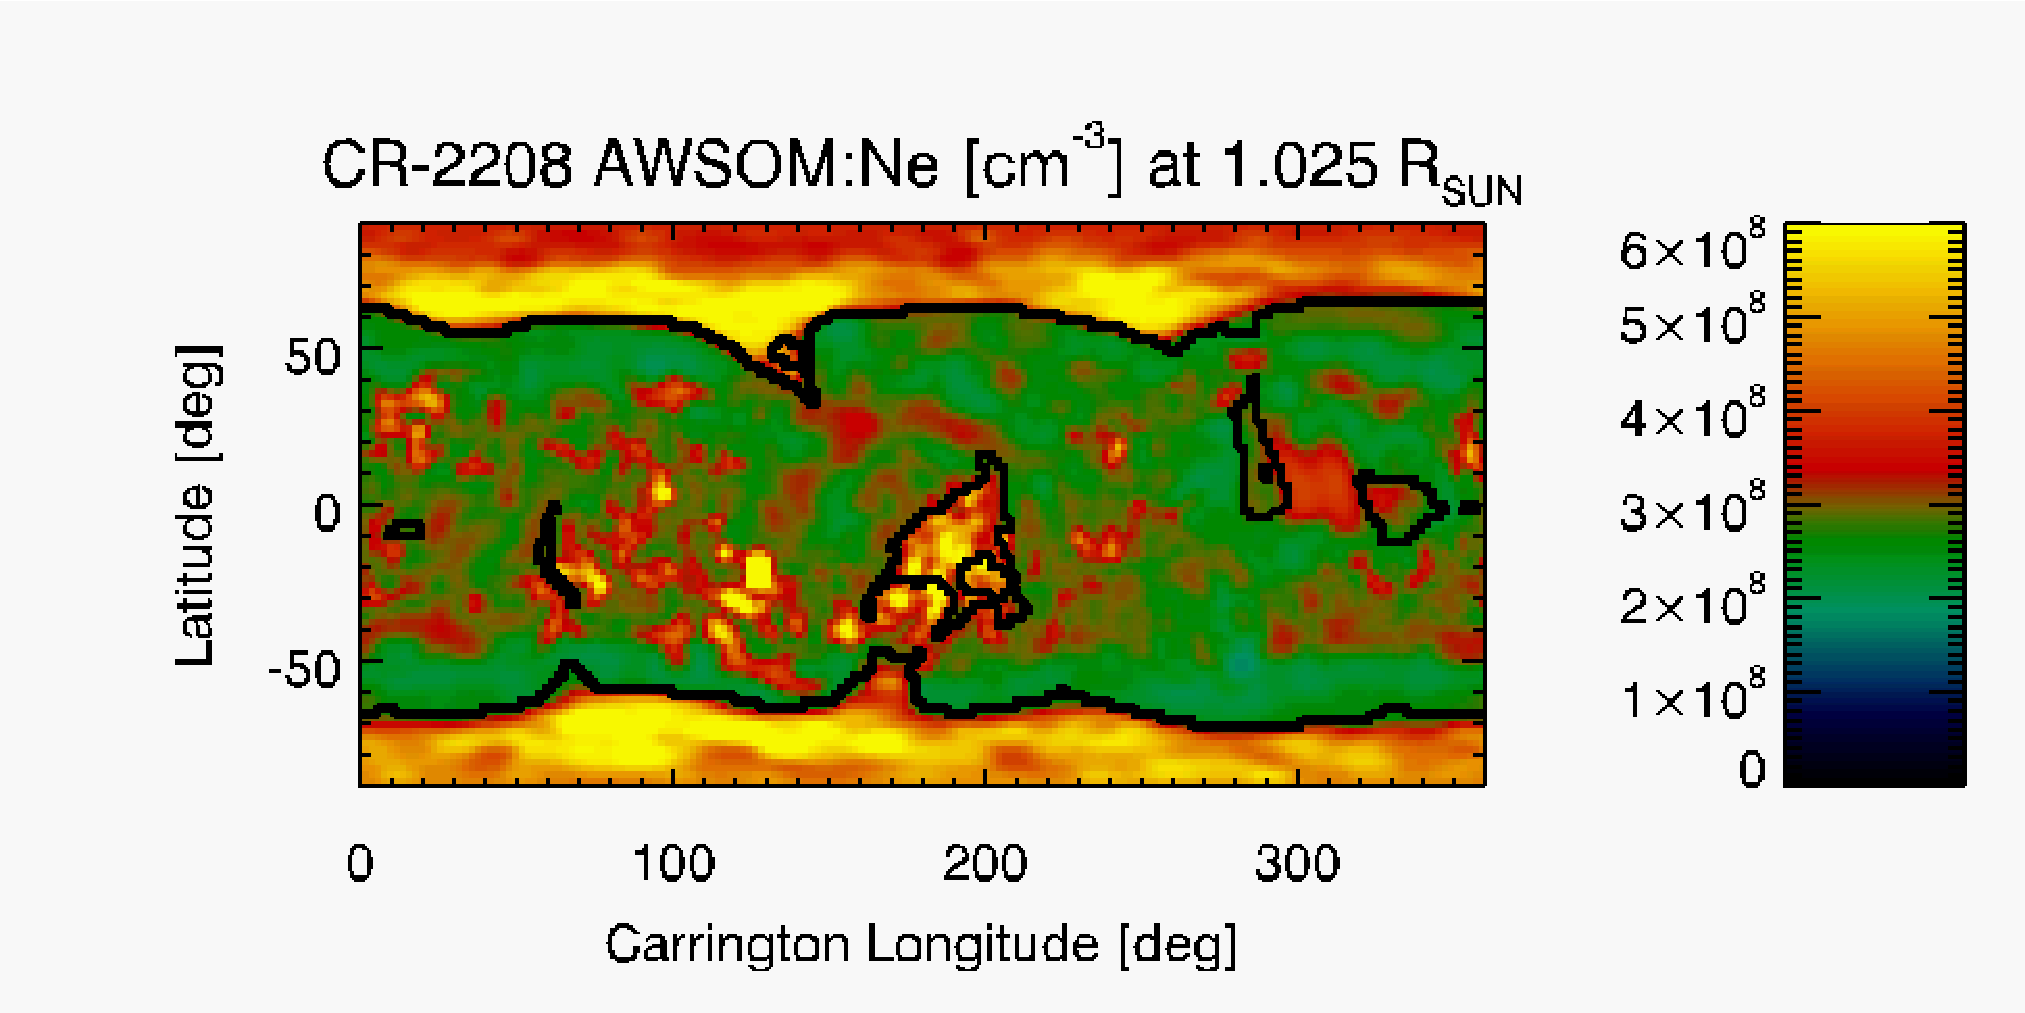
\includegraphics[width=0.495\textwidth]{figs/map_Ne_awsom_2208_185_short_1025_Rsun.pdf}
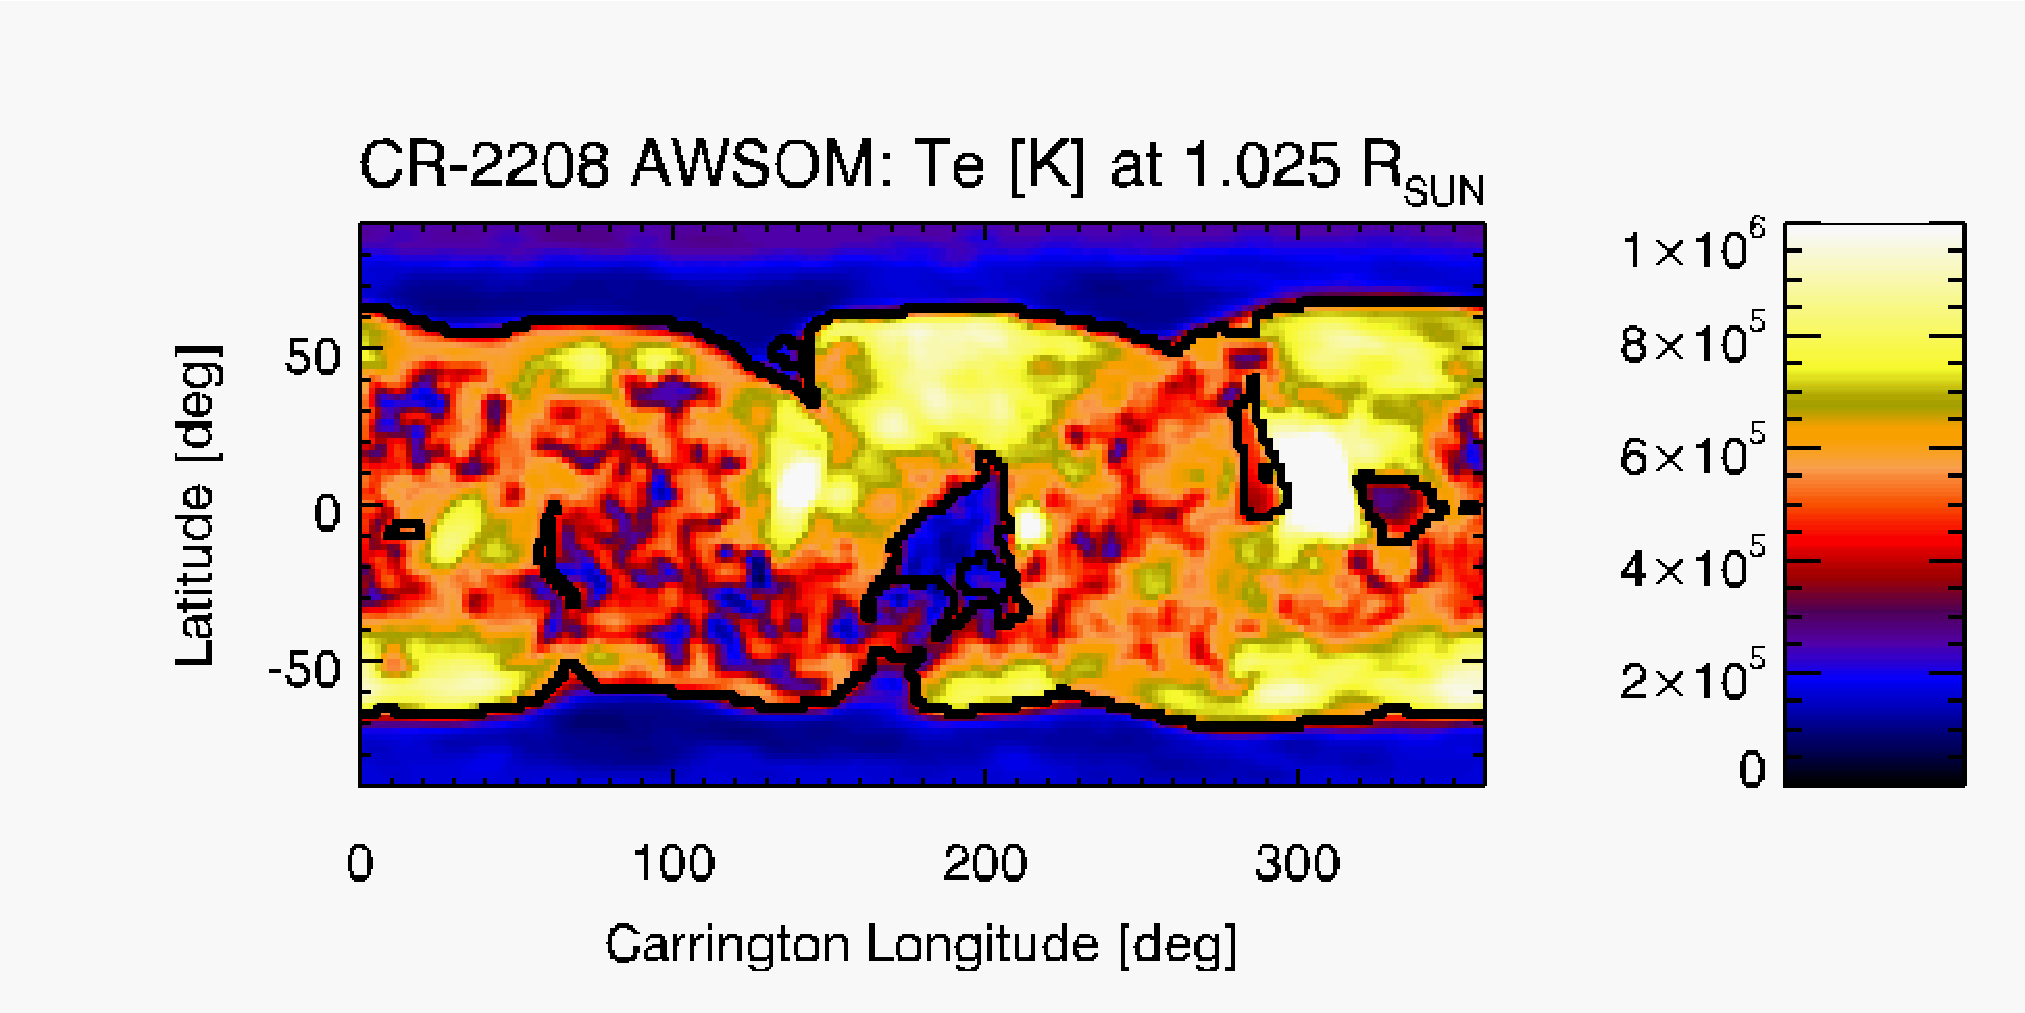
\includegraphics[width=0.495\textwidth]{figs/map_Te_awsom_2208_185_short_1025_Rsun.pdf}
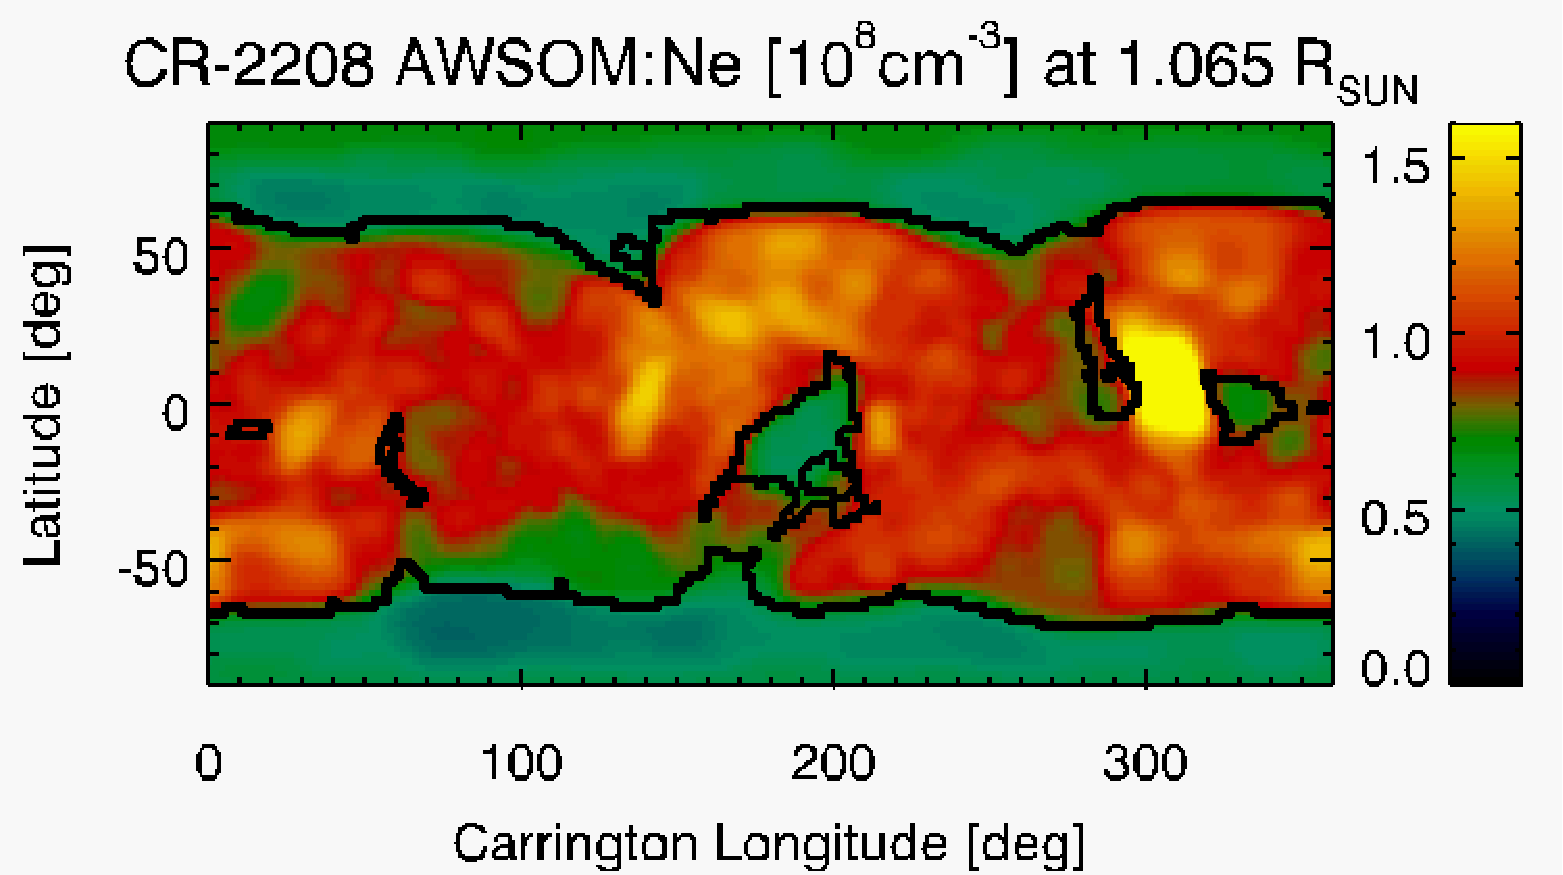
\includegraphics[width=0.495\textwidth]{figs/map_Ne_awsom_2208_185_short_1065_Rsun.pdf}
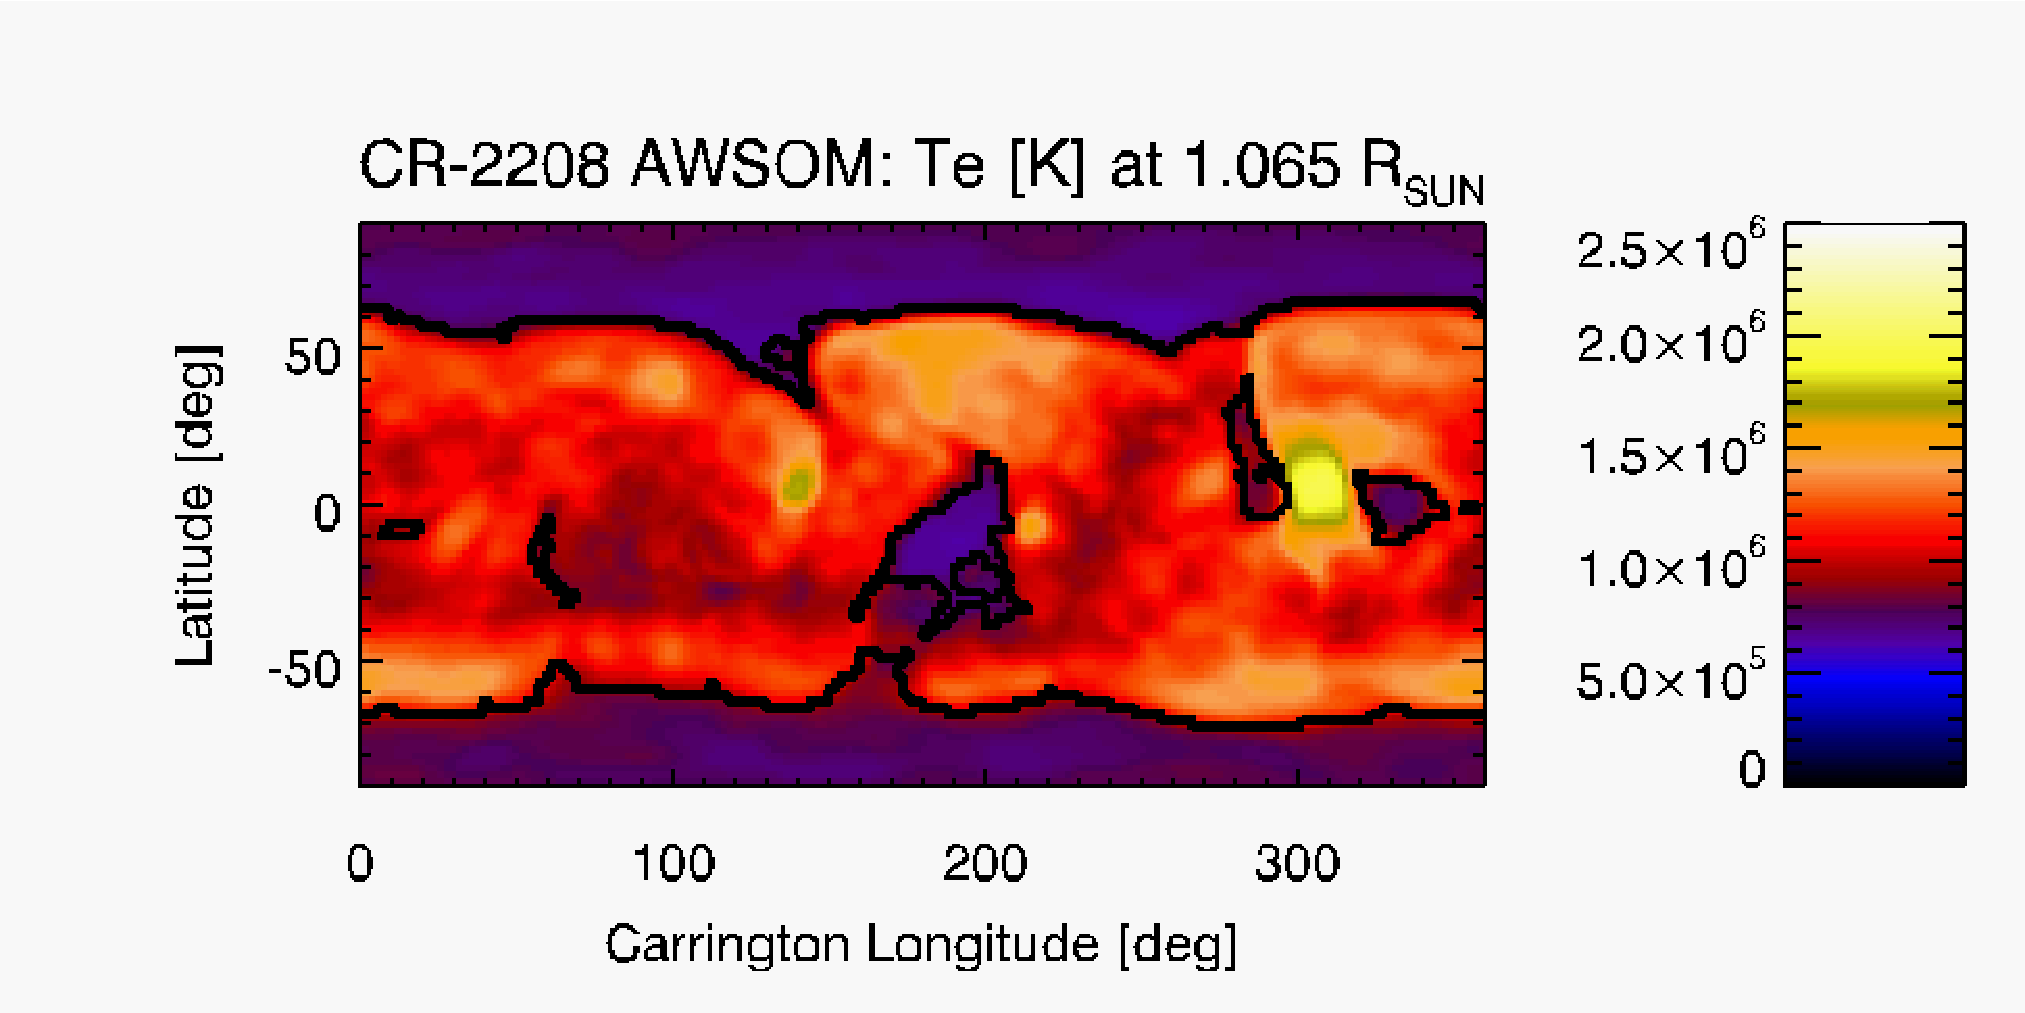
\includegraphics[width=0.495\textwidth]{figs/map_Te_awsom_2208_185_short_1065_Rsun.pdf}
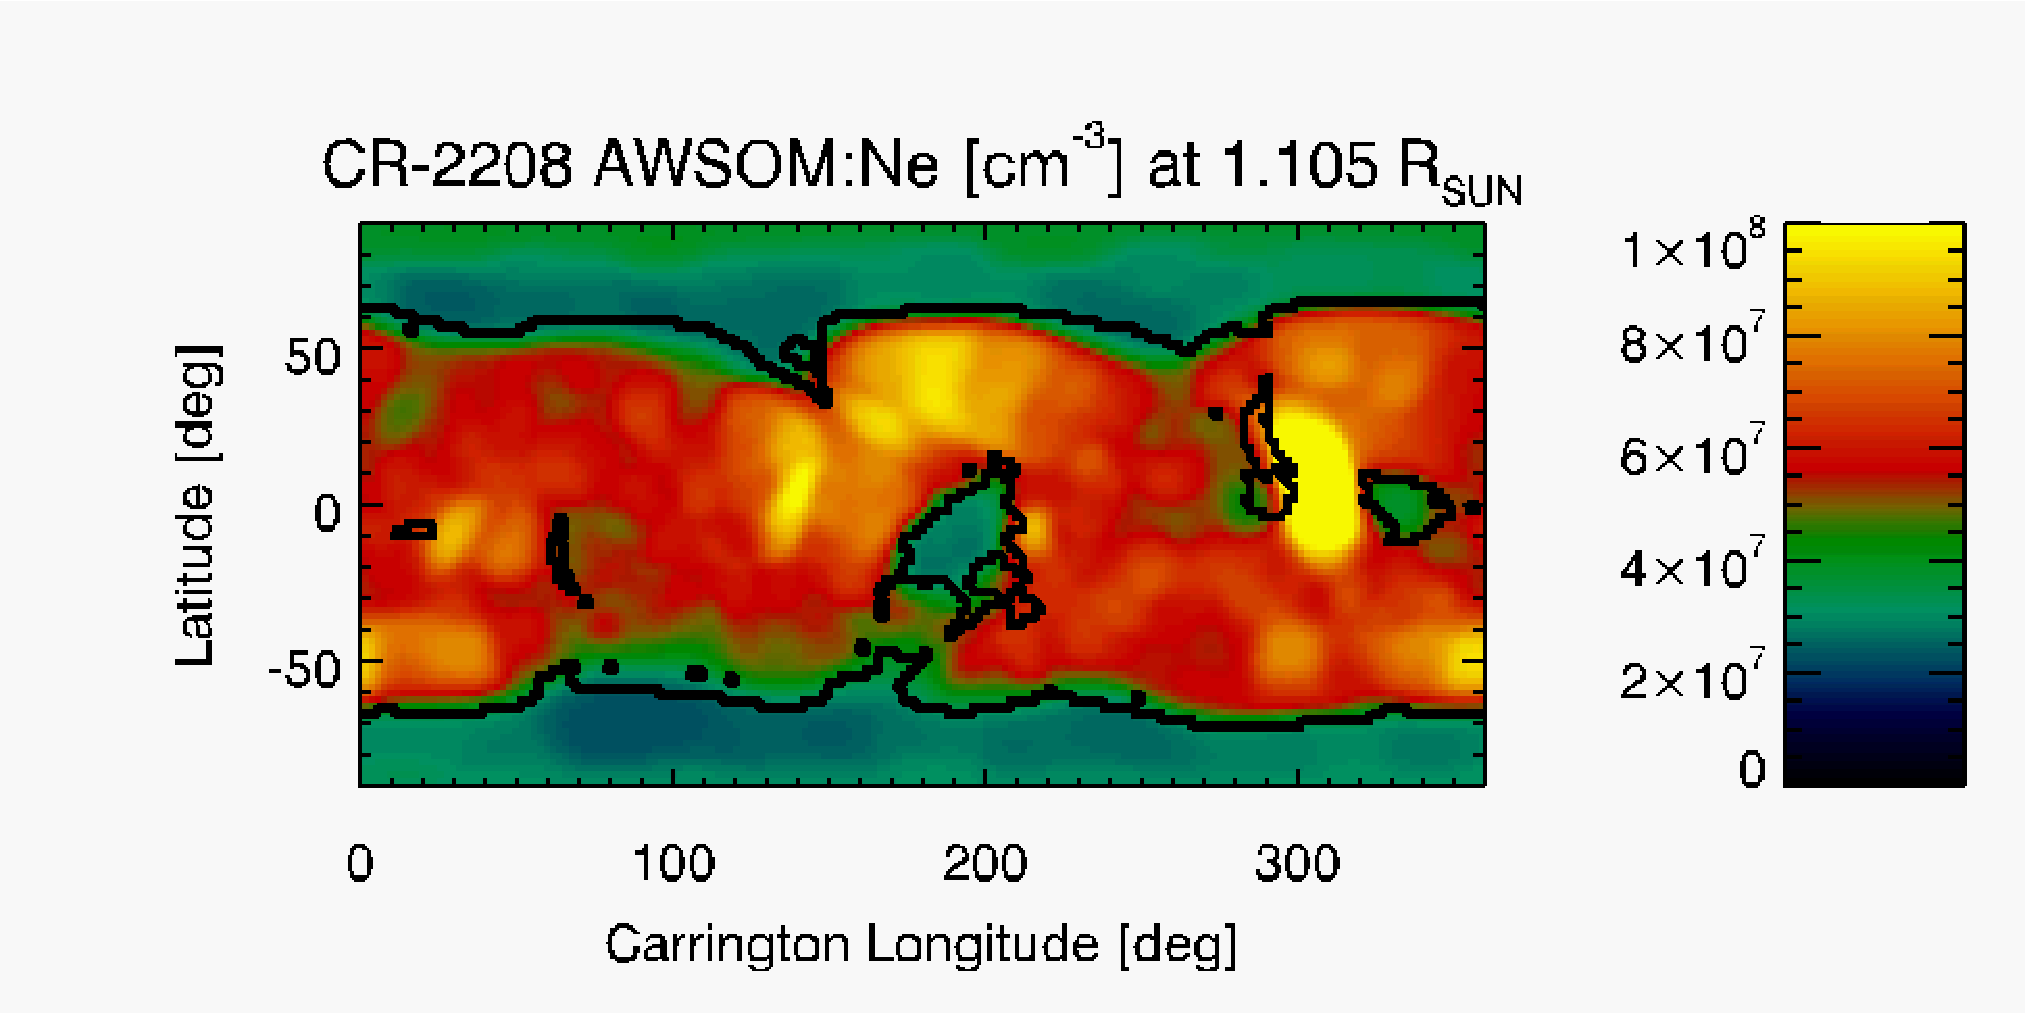
\includegraphics[width=0.495\textwidth]{figs/map_Ne_awsom_2208_185_short_1105_Rsun.pdf}
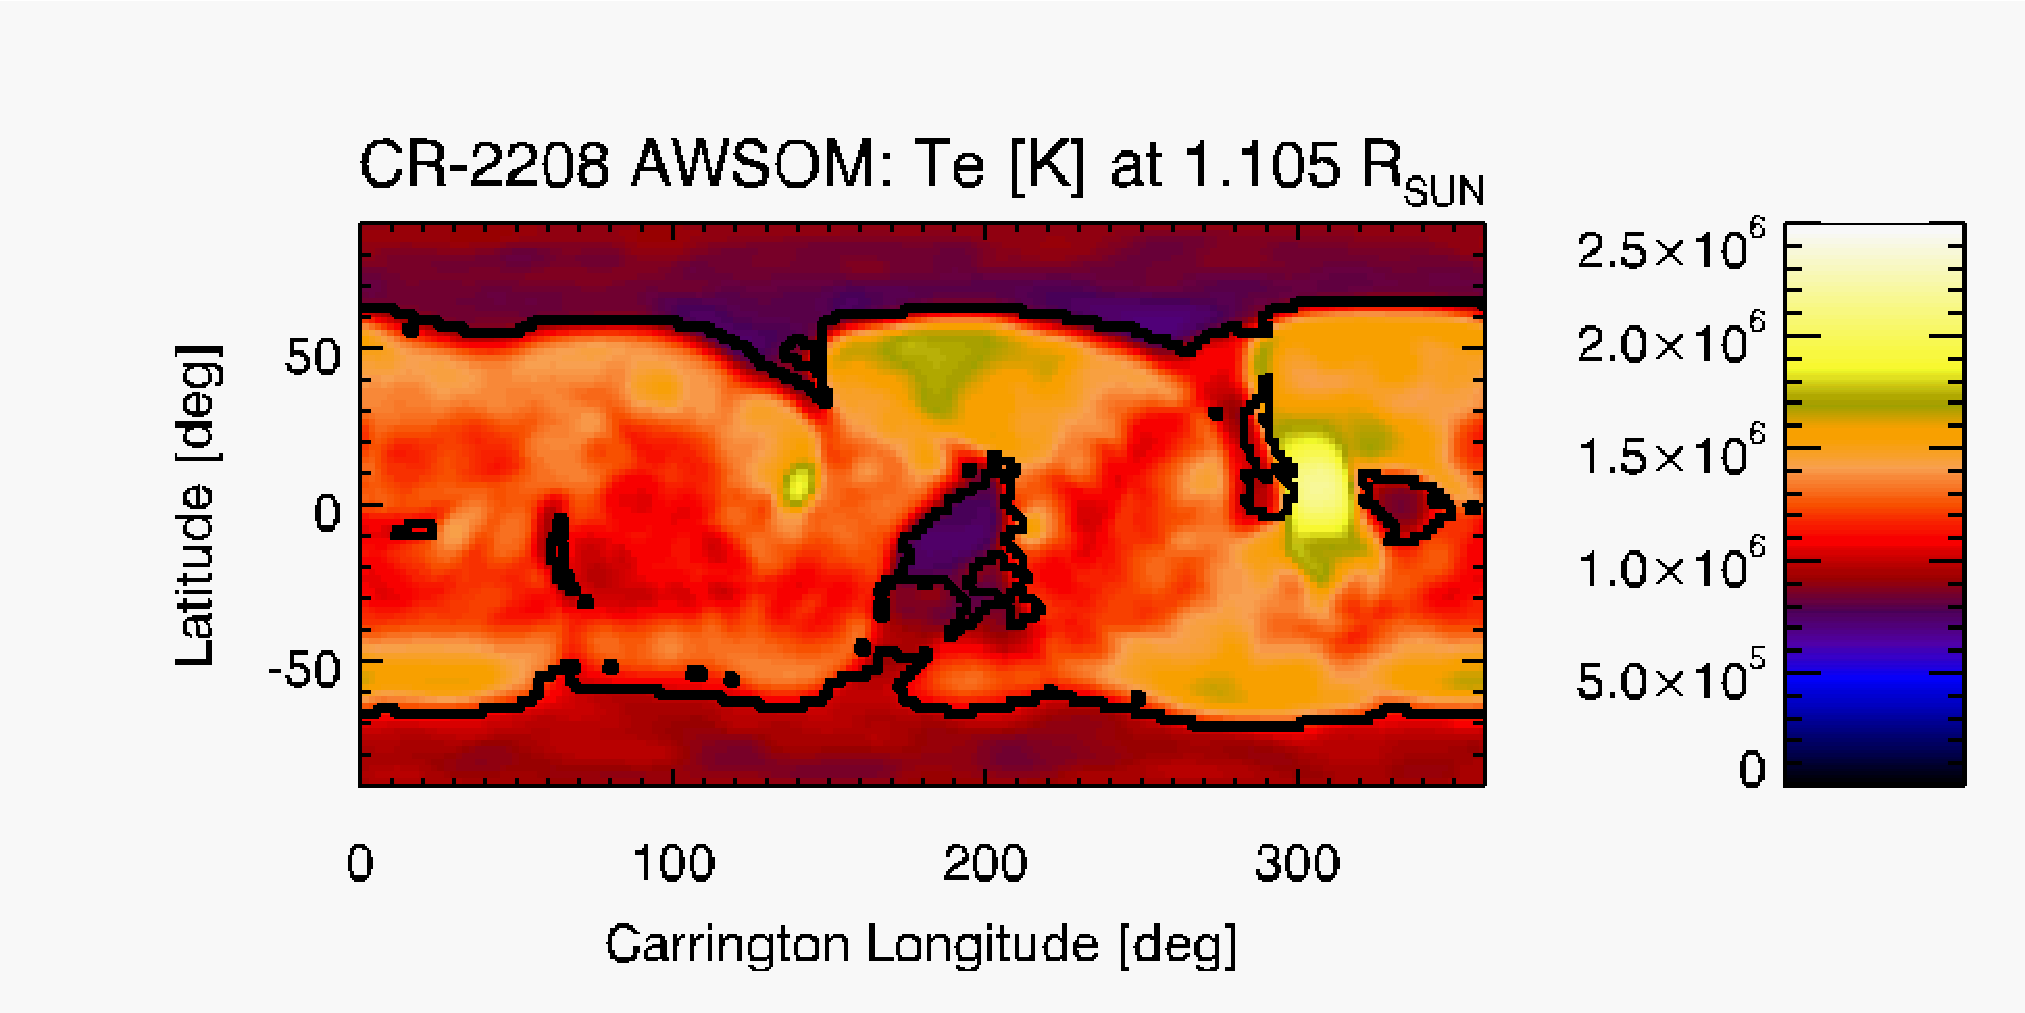
\includegraphics[width=0.495\textwidth]{figs/map_Te_awsom_2208_185_short_1105_Rsun.pdf}
\caption{Same as Figure \ref{carmaps_awsom_2208} for CR-2208.}
\label{carmaps_awsom_2208}
\end{center}
\end{figure}

\textcolor{red}{Se presentan los midpoints para awsom que lucen mas rellenos xq no hay down loops y todo es super suave.}

\begin{figure}[h!]
\begin{center}
%\includegraphics[width=0.495\textwidth,clip=]{Highpoint_2082_demt_paper_Rpoint-map.eps}
\includegraphics[width=0.495\textwidth,clip=]{figs/Highpoint_2082_awsom_paper_cr2082_up_Rpoint-map.eps}
%\includegraphics[width=0.495\textwidth,clip=]{Highpoint_2208_demt_paper_Rpoint-map.eps}
\includegraphics[width=0.495\textwidth,clip=]{figs/Highpoint_2208_awsom_paper_cr2208_up_Rpoint-map.eps}
\caption{Same as Figure \ref{rpoint_demt}, using the density and temperature of AWSoM model to classify legs in type 1, 2 and 3.}
\label{rpoint_awsom}
\end{center}
\end{figure} 

\begin{figure}[h!]
\begin{center}
\includegraphics[width=0.495\textwidth]{figs/Perfil_Ne_demt_awsom_2082_1105.eps}
\includegraphics[width=0.495\textwidth]{figs/Perfil_Ne_demt_awsom_2208_1105.eps}
\includegraphics[width=0.495\textwidth]{figs/Perfil_Te_demt_awsom_2082_1105.eps}
\includegraphics[width=0.495\textwidth]{figs/Perfil_Te_demt_awsom_2208_1105.eps}
\caption{Longitude-averaged electron density (top) and temperature (bottom) for DEMT (blue) and AWSoM (red) results at $1.105\,\mrsun$. The left (right) panels correspond to CR-2082 (CR2208). The vertical black line indicates the longitude-averaged latitudes of the open/close magnetic boundary.}
\label{perf_lon_ne}
\end{center}
\end{figure}



\begin{figure}[h!]
\begin{center}
\includegraphics[width=0.495\textwidth,clip=]{figs/perfil_paper_ne_cr2082_up_short.eps}
\includegraphics[width=0.495\textwidth,clip=]{figs/perfil_paper_te_cr2082_up_short.eps}
\includegraphics[width=0.495\textwidth,clip=]{figs/perfil_paper_ne_cr2208_up_short.eps}
\includegraphics[width=0.495\textwidth,clip=]{figs/perfil_paper_te_cr2208_up_short.eps}
\caption{Average fits of $N_e(r)$ and $T_e(r)$ for all legs of type I (blue), type II (red) and type III (green) for CR-2082 (top panel) and CR-2208 (bottom panel) using DEMT (solid) and AWSoM (dashed) results.}
\label{perfiles_promedio}
\end{center}
\end{figure} 

\textcolor{red}{
As way of example, Figure \ref{histos_2082} and \ref{histos_2208} shows the statistical results of both rotations for the three types of field lines traced with DEMT (blue) and AWSoM results (red). From left to right the panels show the statistical distribution of $\NCB$, $\lN$, $\aTm$ and $B_{\rm CB}$. }


\begin{figure}[h!]
\begin{center}
\includegraphics[width=0.31\textwidth,clip=]{figs/histo_2082_demt_awsom_streamer_up_ne_1055.eps}
\includegraphics[width=0.31\textwidth,clip=]{figs/histo_2082_demt_awsom_streamer_up_lambda_n.eps}
\includegraphics[width=0.31\textwidth,clip=]{figs/histo_2082_demt_awsom_streamer_up_Tm.eps}
\includegraphics[width=0.31\textwidth,clip=]{figs/histo_2082_demt_awsom_bound_up_ne_1055.eps}
\includegraphics[width=0.31\textwidth,clip=]{figs/histo_2082_demt_awsom_bound_up_lambda_n.eps}
\includegraphics[width=0.31\textwidth,clip=]{figs/histo_2082_demt_awsom_bound_up_Tm.eps}
\includegraphics[width=0.31\textwidth,clip=]{figs/histo_2082_demt_awsom_CH_up_ne_1055.eps}
\includegraphics[width=0.31\textwidth,clip=]{figs/histo_2082_demt_awsom_CH_up_lambda_n.eps}
\includegraphics[width=0.31\textwidth,clip=]{figs/histo_2082_demt_awsom_CH_up_Tm.eps}
\caption{Comparative statistical distributions for CR-2082 between DEMT (blue) and AWSoM (red). From left to right: the coronal base electron density $N_e(r=1.055\,\mrsun)$, the electron density scale height $\lN$ and the average $\aTm$ along the four types of legs considered in Section \ref{trace}. In each panel the median ($m$) is indicated.}
\label{histos_2082}
\end{center}
\end{figure} 

%For both rotations, all field lines that meet the criteria listed in Section \ref{trace} were separated into the coronal {regions described in Section \ref{regions} and summarized in Table \ref{tabregions}}. For each field line, the data points of electron density and electron mean temperature versus height were fitted to the functions given by Equations 5 and 6 of Section \ref{trace}. As a result, the footpoint electron density $N_0$ and scale height $\lN$ were computed for each field line, as well as the temperature gradient $a=\textrm{d}T_m/\textrm{d}r$, and the height-averaged (along the loop) electron mean temperature $\aTm$. As the DEMT technique studies only coronal conditions, \textit{i.e.} above height $r\approx 1.025\,\mrsun$, the exponential fit to the electron density data versus height was used to compute the {coronal base electron density} here defined as $\NCB\equiv N_e(r=1.025\,\mrsun)$. Also, for each field line the coronal base magnetic field strength $B_{\rm CB}\equiv B(r=1.025\,\mrsun)$ and its height-averaged value along the loop $\left<B\right>$ were also computed.

\begin{figure}[h!]
\begin{center}
\includegraphics[width=0.31\textwidth,clip=]{figs/histo_2208_demt_awsom_streamer_up_ne_1055.eps}
\includegraphics[width=0.31\textwidth,clip=]{figs/histo_2208_demt_awsom_streamer_up_lambda_n.eps}
\includegraphics[width=0.31\textwidth,clip=]{figs/histo_2208_demt_awsom_streamer_up_Tm.eps}\\
\includegraphics[width=0.31\textwidth,clip=]{figs/histo_2208_demt_awsom_bound_up_ne_1055.eps}
\includegraphics[width=0.31\textwidth,clip=]{figs/histo_2208_demt_awsom_bound_up_lambda_n.eps}
\includegraphics[width=0.31\textwidth,clip=]{figs/histo_2208_demt_awsom_bound_up_Tm.eps}\\
\includegraphics[width=0.31\textwidth,clip=]{figs/histo_2208_demt_awsom_CH_up_ne_1055.eps}
\includegraphics[width=0.31\textwidth,clip=]{figs/histo_2208_demt_awsom_CH_up_lambda_n.eps}
\includegraphics[width=0.31\textwidth,clip=]{figs/histo_2208_demt_awsom_CH_up_Tm.eps}
\caption{Same as Figure \ref{histos_2082} for CR-2208.}
\label{histos_2208}
\end{center}
\end{figure} 


%This plot (E) has never been shown before and I believe it is a very nice result. There are of course previous studies on this, but this would be the first time this is evaluated with tomography. It is not the terminal speed, but it already shows the fast/slow components. We can show this, or we can go for more. Diego can QUANTIFY the correlation by carefully mapping all open field lines at 6 Rsun down to the DEMT region. He needs to code a bit more to achieve this goal, but we believe it is worth. With that tool done Diego can explore other terminal values of quantities of the AWSoM model and the DEMT results below (expansion factor maybe?). This will be nice to do also for the July-2-2019 Eclipse rotation that we will analyze after this paper. 

Visual inspection of the results for CR-2082 in Figure \ref{carmaps_demt_2082} and \ref{carmaps_awsom_2082} reveals two clearly distinct thermodynamical states between the streamer (closed field lines) and the coronal holes (open lines). \\

Figure \ref{perf_lon_ne} shows for both rotations the DEMT and AWSoM longitude-averaged variation of the electron density at the height $r=1.105\,\mrsun$. Density shows higher values in the low-latitudes of the streamer and a nearly monotonic decrease towards the poles. The vertical black lines indicates the longitude-averaged latitudes of the open/close magnetic boundaries (excluding the AR in the case of CR-2082)



Figure \ref{perf_lon_vr} show the longitude-averaged AWSoM radial wind speed $V_r$ at $6\,\mrsun$, where all field lines are open. The heliocentric current sheet (HCS) location is indicated by the minimum of the speed curve.\\

Everything to the south of the HCS maps down to the southern open region in the Figures \ref{perf_lon_ne}, and the same for the northern hemisphere, showing an anti-correlation between $N_e$ at low heights and $V_r$.


\begin{figure}[h!]
\begin{center}
\includegraphics[width=0.495\textwidth]{figs/Perfil_Vr_2082_5995.eps}
\includegraphics[width=0.495\textwidth]{figs/Perfil_Vr_2208_5995.eps}
\caption{Longitude-averaged of radial wind speed at $6\,\mrsun$ given by AWSoM for both rotations.}
\label{perf_lon_vr}
\end{center}
\end{figure}



\section{Discussion}\label{discu} 
%% Figure 
%
% \begin{figure} 
% \centerline{\includegraphics[width=0.5\textwidth,clip=]{<fig.eps>}}
% \caption{}%\label{fig:?}
% \end{figure}



%% Table
%
% \begin{table}
% \caption{}%\label{tbl:?}
% \begin{tabular}{}     
% \hline
% \multicolumn{2}{c}{<>}
% <data>
% \hline
% \end{tabular}
% \end{table}
  

%%%%%%%%%%%%%%%%%%%%%%%%%%%%%%%%%%%%%%%%%%%%%%%%%%%%%%%%%%%%%%%%%%%%%%%%%%%
%% Appendix
%
% \appendix   



%%%%%%%%%%%%%%%%%%%%%%%%%%%%%%%%%%%%%%%%%%%%%%%%%%%%%%%%%%%%%%%%%%%%%%%%%%%
%% Acknowledgements
%
% \begin{acks}
%
% \end{acks}


%%% %%%%%%%%%%%%%%%%%%%%%%%%%%%%%%%%%%%%%%%%%%%%%%%%%%%%%%%%%%%
%% Bibliography
%
% Using BibTeX
%
\bibliographystyle{spr-mp-sola}
\bibliography{solphys_dglloveras}  
%
% Without BibTeX 
% \begin{thebibliography}{}
% \bibitem[\protect\citeauthoryear{Author}{Year}]{key}
%   <bibliographical entry>
%
% \bibitem[\protect\citeauthoryear{}{}]{}
%   
%  
% \end{thebibliography}

\end{article} 
\end{document}
